% =============================================================================================
% Rapport du projet de machine learning
% IA agentique pour la décision d'investissement multicritère
% École Centrale Casablanca, 2026
% Compilation : pdflatex main ; bibtex main ; pdflatex main ; pdflatex main   (ou latexmk -pdf main)
% Compatible Overleaf (compilateur pdfLaTeX).
% =============================================================================================
\documentclass[11pt,a4paper]{report}

% ---------------------------------------------------------------- encodage, langue, police
\usepackage[utf8]{inputenc}
\usepackage[T1]{fontenc}
\usepackage{lmodern}
% Latin Modern n'a pas de petites capitales grasses : on emprunte celles des polices EC.
\DeclareFontShape{T1}{lmr}{bx}{sc}{<->ssub*cmr/bx/sc}{}
\DeclareFontShape{T1}{lmr}{b}{sc}{<->ssub*cmr/bx/sc}{}
\usepackage[french]{babel}
% Expansion des polices désactivée : elle ralentit fortement la compilation (temps limité sur Overleaf).
\usepackage[protrusion=true,expansion=false]{microtype}

% ---------------------------------------------------------------- mise en page
\usepackage[a4paper,top=2.5cm,bottom=2.5cm,left=2.5cm,right=2.5cm,headheight=24pt,headsep=14pt]{geometry}
\usepackage{setspace}
\setstretch{1.12}
\usepackage{fancyhdr}
\usepackage{titlesec}
\usepackage{enumitem}
\setlist{itemsep=2pt,topsep=4pt}

% ---------------------------------------------------------------- figures, tableaux, couleurs
\usepackage{graphicx}
\graphicspath{{figures/}}
\usepackage{booktabs,longtable,array,tabularx,multirow}
\usepackage{float}
\usepackage[font=small,labelfont=bf,labelsep=period]{caption}
\usepackage{subcaption}
\usepackage[table]{xcolor}
\definecolor{eccvert}{HTML}{02987D}
\definecolor{eccgris}{HTML}{72777A}
\definecolor{eccfonce}{HTML}{2B3134}
\definecolor{eccclair}{HTML}{E3F3EF}
\definecolor{ambre}{HTML}{D39B2A}
\definecolor{rouge}{HTML}{C0503F}
\usepackage{tikz}
\usetikzlibrary{arrows.meta,positioning,shapes.geometric,fit,calc,backgrounds}

% ---------------------------------------------------------------- mathématiques
\usepackage{amsmath,amssymb,amsthm,bm}
\DeclareMathOperator*{\argmax}{arg\,max}
\DeclareMathOperator*{\argmin}{arg\,min}

% ---------------------------------------------------------------- encadrés, code, liens
\usepackage{tcolorbox}
\newtcolorbox{encadre}[1][]{colback=eccclair,colframe=eccvert,boxrule=0.6pt,arc=2pt,left=6pt,right=6pt,
  top=4pt,bottom=4pt,fonttitle=\bfseries\small,title={#1}}
\newtcolorbox{definition}[1][]{colback=white,colframe=eccgris,boxrule=0.5pt,arc=2pt,left=6pt,right=6pt,
  top=3pt,bottom=3pt,fonttitle=\bfseries\small,coltitle=eccfonce,colbacktitle=eccclair,title={#1}}
\usepackage{listings}
\lstset{basicstyle=\ttfamily\small,breaklines=true,frame=single,rulecolor=\color{eccgris},
  backgroundcolor=\color{eccclair!40},columns=fullflexible,keepspaces=true}
\usepackage[hidelinks]{hyperref}
\hypersetup{colorlinks=true,linkcolor=eccfonce,citecolor=eccvert,urlcolor=eccvert,
  pdftitle={IA agentique pour la décision d'investissement multicritère},
  pdfauthor={Mathieu, Adingra, Serge, Sarah}}
\usepackage{url}

% ---------------------------------------------------------------- titres et en-têtes
\titleformat{\chapter}[display]{\normalfont\huge\bfseries\color{eccfonce}}
  {\large\color{eccvert}\MakeUppercase{\chaptertitlename}~\thechapter}{6pt}{\Huge}
\titlespacing*{\chapter}{0pt}{-10pt}{24pt}
\titleformat{\section}{\normalfont\Large\bfseries\color{eccfonce}}{\color{eccvert}\thesection}{0.8em}{}
\titleformat{\subsection}{\normalfont\large\bfseries\color{eccfonce}}{\color{eccvert}\thesubsection}{0.8em}{}
\pagestyle{fancy}
\fancyhf{}
\fancyhead[L]{\small\color{eccgris}IA agentique pour la décision d'investissement}
\fancyhead[R]{\small\color{eccgris}\leftmark}
\fancyfoot[C]{\small\thepage}
\renewcommand{\headrulewidth}{0.4pt}
\renewcommand{\headrule}{\hbox to\headwidth{\color{eccvert}\leaders\hrule height \headrulewidth\hfill}}
\fancypagestyle{plain}{\fancyhf{}\fancyfoot[C]{\small\thepage}\renewcommand{\headrulewidth}{0pt}}

% ---------------------------------------------------------------- raccourcis
\newcommand{\pd}{\ensuremath{\mathrm{PD}}}
\newcommand{\code}[1]{\texttt{#1}}
\newcommand{\dollar}{\$}

\begin{document}

% =============================================================================================
% PAGE DE GARDE
% =============================================================================================
\begin{titlepage}
  \begin{center}
    
\includegraphics[width=0.36\textwidth]{logo-ecc.png}\\[0.6cm]
    {\large\color{eccgris}\textsc{École Centrale Casablanca}}\\[0.2cm]
    {\color{eccgris}Projet de machine learning}\\[2.2cm]
    {\color{eccvert}\rule{\linewidth}{1.2pt}}\\[0.5cm]
    {\Huge\bfseries\color{eccfonce} IA agentique pour la décision\\[0.25cm] d'investissement multicritère}\\[0.5cm]
    {\Large\color{eccfonce} Évaluation et sélection de projets d'investissement}\\[0.4cm]
    {\color{eccvert}\rule{\linewidth}{1.2pt}}\\[1.6cm]
    {\large Risque de crédit par apprentissage automatique, décision par ELECTRE III / TRI\\
    et PROMETHEE II, arbitrage sous budget, agents fondés sur un modèle de langage}\\[2.4cm]
    \begin{tabular}{rl}
      \textbf{Équipe} & Mathieu \quad Adingra \quad Serge \quad Sarah\\[0.25cm]
      \textbf{Encadrant} & \textit{à compléter}\\[0.25cm]
      \textbf{Dépôt} & \url{https://github.com/Andj04/D-cision-financi-re}\\
    \end{tabular}
    \par\vfill
    {\large Novembre 2026}
  \end{center}
\end{titlepage}

% =============================================================================================
% PAGES LIMINAIRES
% =============================================================================================
\pagenumbering{roman}
% =============================================================================================
\chapter*{Résumé}
\addcontentsline{toc}{chapter}{Résumé}

Une banque qui finance des projets d'investissement de PME doit arbitrer entre des critères contradictoires
(risque, rentabilité, capacité de remboursement, garanties, impact environnemental et social) sous un budget
limité. Ce projet construit un système d'aide à la décision dans lequel chaque composant a un rôle unique :
\textbf{l'apprentissage automatique estime le risque, une méthode multicritère classe et catégorise, un agent
d'arbitrage respecte le budget, un modèle de langage rédige et répond, et le comité d'investissement décide.}

Le risque de défaut à cinq ans est appris sur 910\,033 prêts réels du programme américain SBA 7(a) (2000-2016),
séparés dans le temps (entraînement 2000-2012, validation 2013-2014, test 2015-2016). Une fuite de données a été
détectée et corrigée : la durée exacte du prêt est modifiée après un défaut. Trois modèles sont comparés sur les
mêmes 13 variables : une régression logistique (AUROC de 0,726 sur le test), un modèle additif interprétable EBM
(0,778) et un modèle de boosting LightGBM (0,800). La règle, fixée avant l'entraînement, retient le meilleur modèle
\emph{interprétable} : l'EBM, calibré par régression isotonique. L'interprétabilité coûte ainsi 0,022 point d'AUROC.

Quarante prêts du test, dont les indicateurs financiers sont simulés à partir des paramètres sectoriels de
Damodaran, forment le portefeuille candidat. Les poids des huit critères sont obtenus par AHP (ratio de cohérence
0,009) ; un filtre éliminatoire écarte 11 projets ; ELECTRE TRI affecte 9 projets à \og Financer \fg{}, 19 à
\og Financer sous conditions \fg{} et 12 à \og Refuser \fg{} ; ELECTRE III et PROMETHEE II donnent des classements
cohérents (Spearman 0,891). Un agent d'arbitrage sélectionne ensuite, sous un budget de 5\,M\$, 11 projets en
respectant le classement, les montants admissibles et un plafond sectoriel de 35\,\%. Les analyses de sensibilité
montrent que les décisions résistent aux paramètres de la méthode mais dépendent fortement de la simulation, ce qui
est la principale limite de la démonstration.

Le système est déployé dans une application Streamlit réutilisable : tout jeu de projets peut y être importé et
évalué avec ses propres critères, poids, filtres et budget. Un agent rédacteur et un conseiller conversationnel,
fondés sur Gemini, n'effectuent aucun calcul : ils appellent des fonctions Python déterministes et chaque nombre de
leurs réponses est vérifié automatiquement.

\medskip
\noindent\textbf{Mots-clés :} risque de crédit, probabilité de défaut, EBM, LightGBM, calibration, fuite de données,
aide multicritère à la décision, AHP, ELECTRE III, ELECTRE TRI, PROMETHEE II, sac à dos, agents LLM, Streamlit.

\tableofcontents
\listoffigures
\listoftables
% =============================================================================================
\chapter*{Abréviations et notations}
\addcontentsline{toc}{chapter}{Abréviations et notations}

\begin{center}
\small
\begin{longtable}{>{\bfseries}p{2.6cm}p{11.8cm}}
\toprule
Sigle & Signification \\
\midrule
\endhead
AHP & \textit{Analytic Hierarchy Process}, méthode de pondération par comparaisons deux à deux \\
AUROC & aire sous la courbe ROC (\textit{Receiver Operating Characteristic}) \\
AUPRC & aire sous la courbe précision-rappel \\
CR & ratio de cohérence de l'AHP (\textit{Consistency Ratio}) \\
DSCR & \textit{Debt Service Coverage Ratio}, flux de trésorerie divisé par le service annuel de la dette \\
EBM & \textit{Explainable Boosting Machine}, modèle additif généralisé interprétable \\
ELECTRE & ÉLimination Et Choix Traduisant la REalité, famille de méthodes de surclassement \\
ESG & Environnement, Social, Gouvernance \\
FOIA & \textit{Freedom of Information Act}, cadre de publication des données de la SBA \\
GAM & modèle additif généralisé (\textit{Generalized Additive Model}) \\
LLM & grand modèle de langage (\textit{Large Language Model}) \\
MCDA & aide multicritère à la décision (\textit{Multiple Criteria Decision Analysis}) \\
ML & apprentissage automatique (\textit{Machine Learning}) \\
NAICS & \textit{North American Industry Classification System}, code d'activité \\
PD, \code{pd\_ml} & probabilité de défaut ; \code{pd\_ml} est celle estimée par le modèle retenu \\
PME & petite ou moyenne entreprise \\
PROMETHEE & \textit{Preference Ranking Organization METHod for Enrichment Evaluations} \\
SBA & \textit{Small Business Administration}, agence fédérale américaine des PME \\
SHAP & \textit{SHapley Additive exPlanations}, explication par valeurs de Shapley \\
TRI & taux de rendement interne \\
VAN & valeur actuelle nette \\
\midrule
$\lambda$ & niveau de coupure d'ELECTRE TRI (crédibilité exigée pour un surclassement) \\
$q_j, p_j, v_j$ & seuils d'indifférence, de préférence et de veto du critère $j$ \\
$b_1, b_2$ & profils limites d'ELECTRE TRI (Refuser $|$ Conditionner, Conditionner $|$ Financer) \\
$\sigma(a,b)$ & crédibilité de l'affirmation « $a$ surclasse $b$ » \\
$\phi(a)$ & flux net de PROMETHEE II \\
\bottomrule
\end{longtable}
\end{center}

\cleardoublepage
\pagenumbering{arabic}

% =============================================================================================
% CORPS
% =============================================================================================
% =============================================================================================
\chapter{Introduction}\label{chap:intro}

\section{Contexte}

Une banque reçoit chaque année des demandes de crédit d'investissement émanant de petites et moyennes entreprises :
un garage qui veut s'équiper, une clinique qui s'agrandit, un transporteur qui renouvelle sa flotte. La banque est le
\emph{financeur} ; les projets appartiennent à des entités extérieures. Ses ressources sont limitées : un montant
global est alloué sur une période donnée, chaque projet doit respecter des montants minimum et maximum, et la banque
souhaite financer des projets variés plutôt que concentrer son risque sur un seul secteur.

Pour chaque dossier, plusieurs dimensions comptent et se contredisent souvent. Un projet très rentable peut être
risqué ; un projet sûr peut créer peu de valeur ou peu d'emplois ; un projet bien garanti peut être mal noté sur le
plan environnemental. La décision est donc par nature \emph{multicritère}. Elle est aussi
\emph{réglementée} : la banque doit pouvoir expliquer un refus et documenter son processus d'octroi, comme le
rappellent les orientations de l'Autorité bancaire européenne sur l'octroi et le suivi des prêts~\cite{eba2020}.

Le sujet proposé est de s'appuyer sur l'\emph{IA agentique} : des agents spécialisés analysent les dossiers,
évaluent chaque critère et proposent un classement argumenté des projets, la décision finale restant aux décideurs
de la banque. Le choix imposé est un modèle de classement en trois catégories : \og à financer \fg{},
\og à financer si\dots{} \fg{} (sous conditions) et \og rejeté \fg{}.

\section{Problématique}

\begin{encadre}[Problématique]
Comment combiner une estimation du risque de défaut apprise sur des données réelles, des critères financiers et
extra-financiers et des contraintes de budget pour proposer, de façon transparente et vérifiable, un classement et
une catégorie pour chaque projet, tout en utilisant des modèles de langage sans leur confier ni calcul ni décision ?
\end{encadre}

Trois difficultés structurent cette question. La première est \emph{statistique} : le défaut est rare (environ 4\,\%
des prêts récents), les données mélangent des périodes de crise et de calme, et une variable peut contenir l'issue
du prêt sans qu'on le voie (fuite de données). La deuxième est \emph{décisionnelle} : les critères sont hétérogènes
(une probabilité, des montants, des ratios, un score) et une mauvaise note sur un critère essentiel ne doit pas être
rachetée par de bonnes notes ailleurs. La troisième est \emph{de confiance} : un modèle de langage rédige bien mais
peut inventer des chiffres, ce qui est inacceptable dans un dossier de crédit.

\section{Objectifs}

\begin{enumerate}
  \item Construire une variable de défaut à cinq ans fiable à partir de prêts réels et ouverts (programme SBA 7(a)),
        sans fuite d'information.
  \item Comparer un modèle de référence simple et des modèles plus avancés, les calibrer, mesurer leurs
        performances sur des années futures et expliquer leurs prédictions.
  \item Évaluer un portefeuille de projets candidats sur huit critères par une méthode multicritère non
        compensatoire (ELECTRE III et ELECTRE TRI), vérifiée par une seconde méthode (PROMETHEE II), avec des poids
        cohérents (AHP) et un filtre éliminatoire.
  \item Sélectionner les projets à financer sous un budget global, des bornes de montant et un plafond sectoriel.
  \item Mesurer la robustesse des décisions aux paramètres de la méthode et aux données simulées.
  \item Ajouter des agents fondés sur un modèle de langage qui rédigent et expliquent sans jamais calculer.
  \item Livrer une solution déployée, réutilisable sur d'autres jeux de projets, reproductible et documentée.
\end{enumerate}

\section{Principe directeur}

Le projet repose sur une séparation stricte des rôles, retenue dès la conception :

\begin{encadre}[Qui fait quoi]
\textbf{L'apprentissage automatique ne calcule que le risque.} \textbf{La méthode multicritère classe et catégorise.}
\textbf{L'agent d'arbitrage respecte le budget.} \textbf{Le modèle de langage rédige et répond, il ne calcule jamais.}
\textbf{Le comité d'investissement fixe les paramètres en amont et décide en aval.}
\end{encadre}

Cette séparation a deux avantages. Chaque composant peut être testé et justifié séparément, et chaque chiffre d'une
recommandation peut être retracé jusqu'aux données et aux paramètres qui l'ont produit.

\section{Contributions}

\begin{itemize}
  \item Un pipeline reproductible sur 910\,033 prêts SBA, avec un audit des données, une séparation temporelle et la
        détection d'une fuite de données non documentée (la durée exacte du prêt).
  \item Une comparaison de trois modèles qui chiffre le \emph{prix de l'interprétabilité} : 0,022 point d'AUROC entre
        le meilleur modèle interprétable (EBM) et un modèle de boosting opaque (LightGBM).
  \item Un moteur multicritère implémenté et testé à la main (AHP, filtre, ELECTRE III avec distillation, ELECTRE TRI,
        PROMETHEE II, sensibilité sur 200 scénarios et 20 tirages de simulation).
  \item Un agent d'arbitrage sous budget, avec deux règles de sélection comparées.
  \item Deux agents fondés sur un modèle de langage, dont un conseiller qui appelle dix outils de calcul, avec un
        vérificateur automatique des nombres et des noms de méthodes.
  \item Une application Streamlit déployée et un moteur générique qui évalue n'importe quel jeu de projets.
\end{itemize}

\section{Plan du rapport}

Le chapitre~\ref{chap:theorie} présente les fondements théoriques de toutes les méthodes utilisées. Le
chapitre~\ref{chap:donnees} décrit les données, leur nettoyage et l'analyse exploratoire. Le
chapitre~\ref{chap:methodo} expose l'architecture du système et la méthodologie. Le chapitre~\ref{chap:resultats}
présente les résultats. Le chapitre~\ref{chap:solution} décrit la solution déployée. Le
chapitre~\ref{chap:discussion} discute les choix, les limites et les perspectives, avant la conclusion.

% =============================================================================================
\chapter{Fondements théoriques}\label{chap:theorie}

Ce chapitre présente les concepts, méthodes et algorithmes utilisés, dans l'ordre de la chaîne de décision :
le risque de crédit et les indicateurs financiers, l'apprentissage supervisé et son évaluation, l'interprétabilité,
l'aide multicritère à la décision, la sélection sous budget et les agents fondés sur des modèles de langage.

% ---------------------------------------------------------------------------------------------
\section{Risque de crédit}

\subsection{Défaut et probabilité de défaut}

Un emprunteur fait \emph{défaut} lorsqu'il ne rembourse pas sa dette et que la banque constate une perte. Dans les
données de la SBA, un prêt passé en perte porte le statut \code{CHGOFF} (\textit{charged off}). La \emph{probabilité de
défaut} (PD) est la probabilité qu'un emprunteur fasse défaut sur un horizon donné. Avec la perte en cas de défaut
et l'exposition, elle compose la perte attendue, au cœur de la gestion du risque de crédit et de la réglementation
bâloise~\cite{bcbs2006}.

\begin{definition}[Variable cible]
Pour chaque prêt $i$, on définit $y_i = 1$ si le prêt est passé en perte au plus 60 mois après son premier
versement, et $y_i = 0$ sinon. L'horizon de cinq ans correspond à celui d'un crédit d'investissement.
\end{definition}

\subsection{Scoring de crédit}

Le \emph{scoring} attribue à chaque demande un score de risque à partir de caractéristiques connues au moment de la
demande~\cite{thomas2002}. On attend du score deux qualités distinctes : bien \emph{ordonner} les emprunteurs du plus
sûr au plus risqué (discrimination), et donner des probabilités \emph{fiables} au sens où, parmi les emprunteurs à
qui l'on attribue 5\,\%, environ 5\,\% font défaut (calibration). Dans notre système, la seconde qualité est aussi
importante que la première, car la méthode multicritère et le filtre éliminatoire utilisent la valeur de la
probabilité, pas seulement le rang.

% ---------------------------------------------------------------------------------------------
\section{Indicateurs financiers d'un projet}\label{sec:indicateurs}

\subsection{Valeur actuelle nette}

Un projet nécessite un investissement initial $I_0$ et génère des flux de trésorerie $F_t$ aux années
$t = 1, \dots, T$. Un dirham reçu dans le futur vaut moins qu'un dirham aujourd'hui : on \emph{actualise} les flux au
taux $r$, égal au coût du capital du secteur. La valeur actuelle nette est
\begin{equation}
  \mathrm{VAN} = -I_0 + \sum_{t=1}^{T} \frac{F_t}{(1+r)^t} + \frac{V_T}{(1+r)^T},
\end{equation}
où $V_T$ est la valeur résiduelle du projet après l'horizon explicite. Une VAN positive signifie que le projet crée
de la valeur au-delà de la rémunération exigée par les apporteurs de capitaux. Le taux de rendement interne (TRI) est
le taux $r$ qui annule la VAN.

\subsection{Délai de récupération}

Le délai de récupération est le nombre d'années nécessaires pour que les flux cumulés remboursent
l'investissement :
\begin{equation}
  D = \min \Big\{ \tau : \sum_{t=1}^{\tau} F_t \geq I_0 \Big\},
\end{equation}
interpolé linéairement à l'intérieur de l'année de récupération. C'est une mesure de liquidité et de risque : plus
il est court, plus la banque est vite exposée à un projet qui a déjà remboursé sa mise.

\subsection{Ratio de couverture du service de la dette}

Le DSCR rapporte le flux de trésorerie d'une année au service de la dette de cette année (intérêts et
remboursement du capital) :
\begin{equation}
  \mathrm{DSCR}_t = \frac{F_t}{S_t}, \qquad S = K\,\frac{i}{1-(1+i)^{-n}},
\end{equation}
où $S$ est l'annuité constante d'un prêt de montant $K$ au taux $i$ sur $n$ années. Un DSCR inférieur à 1 signifie
que le projet ne génère pas assez de trésorerie pour payer ses échéances. On retient le minimum sur la durée du
prêt, $\mathrm{DSCR}_{\min} = \min_t \mathrm{DSCR}_t$, qui décrit l'année la plus tendue. Les financements de
projets d'énergie renouvelable exigent typiquement un DSCR de 1,25 à 1,40~\cite{nrel2024}.

\subsection{Levier, garanties et critères extra-financiers}

Le \emph{levier} rapporte la dette aux fonds propres apportés par les propriétaires : plus il est élevé, moins
l'entreprise peut absorber une perte. La \emph{couverture par les garanties} rapporte la valeur des sûretés au
montant prêté ; une couverture de 1 signifie que les garanties valent le prêt. Les orientations de
l'ABE~\cite{eba2020} rappellent que la garantie est un second recours qui ne doit pas fonder la décision, d'où un
poids modéré. Le \emph{score ESG} résume les risques environnementaux et sociaux ; les Principes de
l'Équateur~\cite{equator2020} classent les projets en catégories A (impacts importants), B (limités) et C (minimes).
Enfin, le nombre d'\emph{emplois soutenus par million investi} mesure l'impact économique local.

% ---------------------------------------------------------------------------------------------
\section{Apprentissage supervisé}

On dispose de $n$ exemples $(\bm{x}_i, y_i)$, où $\bm{x}_i \in \mathbb{R}^d$ décrit le prêt et $y_i \in \{0,1\}$
son issue. On cherche une fonction $\hat p(\bm{x}) \approx \Pr(y = 1 \mid \bm{x})$ qui se généralise à des prêts
futurs.

\subsection{Régression logistique}

La régression logistique modélise le logarithme de la cote par une combinaison linéaire des variables :
\begin{equation}
  \log \frac{\hat p(\bm{x})}{1-\hat p(\bm{x})} = \beta_0 + \bm{\beta}^\top \bm{x},
  \qquad \hat p(\bm{x}) = \frac{1}{1+e^{-(\beta_0 + \bm{\beta}^\top \bm{x})}}.
\end{equation}
Les coefficients minimisent la log-vraisemblance négative régularisée :
\begin{equation}
  \min_{\beta_0,\bm{\beta}} \; -\sum_{i=1}^{n} \Big[ y_i \log \hat p(\bm{x}_i) + (1-y_i)\log\big(1-\hat p(\bm{x}_i)\big) \Big]
  + \frac{1}{2C}\,\|\bm{\beta}\|_2^2 .
\end{equation}
Le paramètre $C$ règle la force de la régularisation (plus $C$ est petit, plus les coefficients sont contraints). Les
variables catégorielles sont codées en indicatrices (\textit{one-hot}) et les variables numériques standardisées.
Simple, stable et lisible, c'est le modèle de référence (\textit{baseline}) du scoring de crédit~\cite{thomas2002}.
Sa limite est de ne capter ni non-linéarité ni interaction sans ingénierie manuelle.

\subsection{Modèles additifs généralisés et EBM}

Un modèle additif généralisé (GAM) remplace chaque terme linéaire par une fonction quelconque d'une variable :
\begin{equation}
  g\big(\mathbb{E}[y \mid \bm{x}]\big) = \beta_0 + \sum_{j=1}^{d} f_j(x_j) + \sum_{(j,k) \in \mathcal{I}} f_{jk}(x_j, x_k),
\end{equation}
où $g$ est la fonction logit et $\mathcal{I}$ un petit ensemble de paires de variables en interaction (modèle
GA$^2$M~\cite{lou2013}). L'\emph{Explainable Boosting Machine} (EBM) de la bibliothèque InterpretML~\cite{nori2019}
apprend chaque fonction $f_j$ par \emph{boosting cyclique} : à chaque tour, elle ajuste un arbre très peu profond sur
une seule variable à la fois, avec un faible taux d'apprentissage, en tournant sur toutes les variables. Les
interactions les plus utiles sont ensuite détectées et ajoutées. L'ensemble est moyenné sur plusieurs
rééchantillonnages (\textit{outer bags}).

Le modèle obtenu est aussi précis que de nombreux modèles opaques, tout en restant une \emph{boîte de verre} : la
prédiction est la somme de contributions lisibles, et chaque fonction $f_j$ peut être tracée pour montrer comment le
risque varie avec la variable. C'est la propriété qui motive son choix pour une décision de crédit.

\subsection{Boosting de gradient et LightGBM}

Le boosting de gradient~\cite{friedman2001} construit un modèle additif d'arbres
$F_M(\bm{x}) = \sum_{m=1}^{M} \nu\, h_m(\bm{x})$ : chaque nouvel arbre $h_m$ est ajusté sur le gradient négatif de
la fonction de perte (ici la perte logistique) par rapport à la prédiction courante, et $\nu$ est le taux
d'apprentissage. LightGBM~\cite{ke2017} est une implémentation très efficace : il discrétise les variables en
histogrammes, fait croître les arbres feuille par feuille (la feuille qui réduit le plus la perte d'abord), traite
nativement les variables catégorielles et propose des techniques d'échantillonnage des observations (GOSS) et de
regroupement de variables (EFB). Ses hyperparamètres principaux sont le nombre de feuilles, le taux d'apprentissage
et le nombre d'arbres, ce dernier étant fixé par \emph{arrêt anticipé} : on arrête d'ajouter des arbres quand la
performance sur un jeu de validation cesse de s'améliorer. Très performant sur les données tabulaires, ce modèle
est en revanche opaque : des centaines d'arbres en interaction ne se lisent pas.

% ---------------------------------------------------------------------------------------------
\section{Évaluation d'un classifieur probabiliste}

\subsection{Matrice de confusion, précision, rappel et F1}

Pour un seuil $s$, on prédit un défaut quand $\hat p(\bm{x}) \geq s$. On compte les vrais positifs (VP), faux
positifs (FP), faux négatifs (FN) et vrais négatifs (VN). La précision $\mathrm{VP}/(\mathrm{VP}+\mathrm{FP})$ est la
part des alertes justes, le rappel $\mathrm{VP}/(\mathrm{VP}+\mathrm{FN})$ la part des défauts détectés, et
\begin{equation}
  F_1 = \frac{2\,\text{précision}\times\text{rappel}}{\text{précision}+\text{rappel}} .
\end{equation}
Le F1 dépend du seuil : nous le choisissons sur la validation, là où le F1 est maximal, puis l'appliquons tel quel
au test.

\subsection{Courbes ROC et précision-rappel}

La courbe ROC trace le taux de vrais positifs contre le taux de faux positifs pour tous les seuils. Son aire, l'AUROC,
a une interprétation directe : c'est la probabilité qu'un emprunteur en défaut tiré au hasard reçoive un score plus
élevé qu'un emprunteur sain tiré au hasard ; 0,5 correspond au hasard et 1 à un classement parfait. Quand la classe
positive est rare, l'AUROC peut paraître élevée alors que les alertes sont peu précises : l'aire sous la courbe
précision-rappel (AUPRC) est alors plus informative~\cite{davis2006}. Sa valeur de référence est le taux de défaut :
un modèle au hasard obtient une AUPRC égale à la proportion de positifs.

\subsection{Score de Brier et calibration}

Le score de Brier~\cite{brier1950} mesure l'écart quadratique moyen entre la probabilité prédite et l'issue :
\begin{equation}
  \mathrm{BS} = \frac{1}{n} \sum_{i=1}^{n} \big(\hat p(\bm{x}_i) - y_i\big)^2 .
\end{equation}
Il récompense à la fois la discrimination et la calibration. Un modèle est \emph{calibré} si
$\Pr(y=1 \mid \hat p = p) = p$ ; on le vérifie par une courbe de calibration qui compare, par tranche de probabilité
prédite, la moyenne prédite et la fréquence observée.

La \emph{calibration isotonique}~\cite{zadrozny2002,niculescu2005} corrige les probabilités par une fonction
croissante $m$ ajustée sur un jeu distinct de celui de l'entraînement :
\begin{equation}
  \hat m = \argmin_{m \text{ croissante}} \sum_{i} \big(y_i - m(\hat p_i)\big)^2 ,
\end{equation}
résolu par l'algorithme \textit{pool adjacent violators}. Elle ne modifie pas l'ordre des prédictions (donc
quasiment pas l'AUROC) mais corrige leur niveau. Elle est indispensable lorsque le taux de défaut de la période
d'entraînement diffère de celui de la période d'usage, ce qui est notre cas.

\subsection{Déséquilibre des classes}

Avec 3 à 13\,\% de défauts selon les périodes, la classe positive est minoritaire. Nous n'avons pas rééquilibré
les données (par sur- ou sous-échantillonnage), car cela fausserait les probabilités dont le MCDA a besoin. Nous
avons préféré des métriques adaptées (AUPRC, Brier), un seuil de décision choisi sur la validation et une calibration.

% ---------------------------------------------------------------------------------------------
\section{Bonnes pratiques : séparation des données et fuites}

\subsection{Séparation temporelle}

Les données sont séparées en trois blocs \emph{avant tout prétraitement} : l'entraînement sert à apprendre, la
validation à régler (hyperparamètres, calibration, seuil, choix du modèle) et le test à mesurer la performance
finale, une seule fois. Une banque prédit l'avenir à partir du passé : la séparation suit donc l'année d'approbation
du prêt, et non un tirage au hasard qui mélangerait des prêts de 2008 et de 2015 et donnerait des performances
trop optimistes. Tout ce qui apprend quelque chose des données (médianes d'imputation, échelles, modalités
connues) est ajusté sur l'entraînement uniquement.

\subsection{Fuite de données}

Une fuite survient lorsqu'une variable contient, directement ou indirectement, une information indisponible au
moment de la prédiction~\cite{kaufman2012}. Le modèle paraît alors excellent mais échouera en usage. Les fuites
évidentes (statut du prêt, date et montant de la perte) se suppriment à la source ; les fuites cachées se détectent
par un résultat trop beau pour être vrai, puis par l'examen de la variable suspecte. Nous en avons trouvé une
(section~\ref{sec:fuite}).

% ---------------------------------------------------------------------------------------------
\section{Interprétabilité}

\subsection{Importance par permutation}

L'importance d'une variable $j$ est la baisse de performance observée quand on mélange au hasard ses valeurs, ce qui
casse son lien avec la cible tout en conservant sa distribution~\cite{breiman2001,fisher2019} :
\begin{equation}
  I_j = \mathrm{AUROC}(\hat p, X) - \frac{1}{K}\sum_{k=1}^{K} \mathrm{AUROC}\big(\hat p, X^{\pi_k(j)}\big),
\end{equation}
où $X^{\pi_k(j)}$ est le jeu de données dont la colonne $j$ a été permutée. La méthode s'applique à tout modèle.

\subsection{Explications natives de l'EBM}

L'EBM étant additif, l'importance d'un terme est la valeur absolue moyenne de sa contribution
$\frac{1}{n}\sum_i |f_j(x_{ij})|$, et l'effet d'une variable se lit directement sur la courbe $f_j$. Pour un prêt
donné, la prédiction se décompose exactement en contributions : on peut nommer les facteurs qui augmentent son risque.

\subsection{Valeurs SHAP}

Pour un modèle opaque, les valeurs SHAP~\cite{lundberg2017} attribuent à chaque variable une part de l'écart entre la
prédiction et la prédiction moyenne, selon la valeur de Shapley de la théorie des jeux coopératifs :
\begin{equation}
  \phi_j(\bm{x}) = \sum_{S \subseteq \{1,\dots,d\}\setminus\{j\}}
  \frac{|S|!\,(d-|S|-1)!}{d!}\Big[ v_{\bm{x}}(S\cup\{j\}) - v_{\bm{x}}(S) \Big],
\end{equation}
où $v_{\bm{x}}(S)$ est la prédiction attendue lorsque seules les variables de $S$ sont connues. Ces valeurs sont les
seules à vérifier simultanément l'efficacité (elles somment à l'écart total), la symétrie et la nullité. Pour les
modèles d'arbres, l'algorithme \textit{TreeSHAP} les calcule exactement en temps polynomial.

% ---------------------------------------------------------------------------------------------
\section{Aide multicritère à la décision}

Une alternative $a$ (un projet) est évaluée sur $m$ critères $g_1(a), \dots, g_m(a)$, chacun à maximiser ou à
minimiser, avec des poids $w_j$. Les méthodes \emph{compensatoires}, comme la somme pondérée, permettent qu'une
mauvaise note soit rachetée par de bonnes notes ailleurs. Les méthodes de \emph{surclassement} de l'école
européenne~\cite{roy1991,figueira2005} limitent cette compensation : une très mauvaise performance sur un critère
peut opposer un \emph{veto}. Pour un dossier de crédit, cette propriété est essentielle : un DSCR très faible ne
devrait pas être effacé par une VAN élevée.

\subsection{Pondération par AHP}

L'\textit{Analytic Hierarchy Process}~\cite{saaty1980} construit les poids à partir de comparaisons deux à deux. Pour
chaque paire de critères $(i,j)$, le décideur indique l'importance relative $a_{ij}$ sur l'échelle de Saaty (1 :
égale importance, 3 : modérée, 5 : forte, 7 : très forte, 9 : extrême, valeurs paires intermédiaires), avec
$a_{ji} = 1/a_{ij}$. Huit critères demandent $8\times7/2 = 28$ jugements. Le vecteur des poids est le vecteur propre
principal de la matrice $A = (a_{ij})$ :
\begin{equation}
  A\,\bm{w} = \lambda_{\max}\,\bm{w}, \qquad \sum_j w_j = 1 .
\end{equation}
Si les jugements étaient parfaitement cohérents ($a_{ik} = a_{ij}a_{jk}$), on aurait $\lambda_{\max} = m$. L'indice
de cohérence $\mathrm{CI} = (\lambda_{\max}-m)/(m-1)$ est rapporté à un indice aléatoire $\mathrm{RI}$ ($1{,}41$ pour
$m = 8$) : le ratio $\mathrm{CR} = \mathrm{CI}/\mathrm{RI}$ doit rester inférieur à 0,10.

\subsection{ELECTRE III}

ELECTRE III~\cite{roy1978} compare les alternatives deux à deux. Chaque critère $j$ reçoit trois seuils : un écart
inférieur au seuil d'indifférence $q_j$ est négligeable, un écart supérieur au seuil de préférence $p_j$ est net, et
un écart supérieur au seuil de veto $v_j$ est rédhibitoire. Pour des critères à maximiser, on note
$\Delta_j = g_j(b) - g_j(a)$ l'avantage de $b$ sur $a$.

\paragraph{Concordance.} Le critère $j$ soutient l'affirmation « $a$ surclasse $b$ » d'autant plus que $b$ ne fait
pas nettement mieux :
\begin{equation}
  c_j(a,b) =
  \begin{cases}
    1 & \text{si } \Delta_j \leq q_j,\\[2pt]
    \dfrac{p_j - \Delta_j}{p_j - q_j} & \text{si } q_j < \Delta_j < p_j,\\[6pt]
    0 & \text{si } \Delta_j \geq p_j,
  \end{cases}
  \qquad
  C(a,b) = \frac{\sum_j w_j\, c_j(a,b)}{\sum_j w_j}.
\end{equation}

\paragraph{Discordance.} Le critère $j$ s'oppose d'autant plus que $b$ fait beaucoup mieux :
\begin{equation}
  d_j(a,b) =
  \begin{cases}
    0 & \text{si } \Delta_j \leq p_j,\\[2pt]
    \dfrac{\Delta_j - p_j}{v_j - p_j} & \text{si } p_j < \Delta_j < v_j,\\[6pt]
    1 & \text{si } \Delta_j \geq v_j .
  \end{cases}
\end{equation}

\paragraph{Crédibilité.} La concordance est atténuée par les critères dont la discordance la dépasse :
\begin{equation}
  \sigma(a,b) = C(a,b) \prod_{j \,:\, d_j(a,b) > C(a,b)} \frac{1 - d_j(a,b)}{1 - C(a,b)} .
\end{equation}
Un veto ($d_j = 1$) annule la crédibilité, quelle que soit la concordance : c'est la non-compensation.

\paragraph{Distillation.} Le classement s'obtient en exploitant la matrice $\sigma$ par deux distillations.
À chaque étape, on fixe un niveau $\lambda_k$ juste en dessous de la plus forte crédibilité restante, avec un seuil
de discrimination $s(\lambda) = 0{,}30 - 0{,}15\,\lambda$, et l'on considère que $a$ surclasse $b$ si
$\sigma(a,b) > \lambda_k$ et $\sigma(a,b) - \sigma(b,a) > s(\sigma(a,b))$. La qualification d'une alternative est
le nombre d'alternatives qu'elle surclasse moins le nombre de celles qui la surclassent. La distillation
\emph{descendante} extrait successivement les meilleures, l'\emph{ascendante} les moins bonnes. Les deux préordres
peuvent différer : une alternative bien placée par l'une et mal placée par l'autre est \emph{incomparable} à une
partie des autres, information propre aux méthodes de surclassement.

\subsection{ELECTRE TRI}

ELECTRE TRI~\cite{yu1992} affecte chaque alternative à une catégorie ordonnée, au lieu de la classer. Les catégories
sont séparées par des \emph{profils limites} : $b_1$ entre Refuser et Conditionner, $b_2$ entre Conditionner et
Financer. On calcule la crédibilité $\sigma(a, b_h)$ et $\sigma(b_h, a)$ comme dans ELECTRE III, puis on la
compare à un niveau de \emph{coupure} $\lambda \in [0{,}5 ; 1]$ : $a$ surclasse $b_h$ si $\sigma(a,b_h) \geq \lambda$.

\begin{itemize}
  \item \textbf{Règle pessimiste} (prudente) : on compare $a$ aux profils du plus exigeant au moins exigeant, et on
        l'affecte à la catégorie juste au-dessus du premier profil qu'il surclasse.
  \item \textbf{Règle optimiste} : on compare $a$ aux profils du moins exigeant au plus exigeant, et on l'affecte à la
        catégorie juste en dessous du premier profil qui lui est strictement préféré.
\end{itemize}
La règle pessimiste n'admet un projet dans une catégorie que s'il en franchit clairement le seuil d'entrée ; elle
correspond à la prudence bancaire.

\begin{figure}[htbp]
\centering
\begin{tikzpicture}[x=1.3cm,y=0.62cm,font=\small]
  \foreach \j/\lab in {1/PD,2/DSCR,3/VAN,4/Délai,5/Levier,6/Garanties,7/ESG,8/Emplois}{
    \draw[eccgris!60] (\j,0) -- (\j,6);
    \node[below,text=eccfonce] at (\j,0) {\lab};}
  \fill[rouge!12] (0.6,0) rectangle (8.4,2);
  \fill[ambre!14] (0.6,2) rectangle (8.4,4);
  \fill[eccvert!12] (0.6,4) rectangle (8.4,6);
  \foreach \j in {1,...,8}{\draw[eccgris!60] (\j,0) -- (\j,6);}
  \draw[rouge,thick] (1,2.1) -- (2,1.8) -- (3,2.2) -- (4,1.9) -- (5,2.1) -- (6,1.8) -- (7,2.0) -- (8,2.2);
  \draw[eccvert,thick] (1,4.0) -- (2,4.2) -- (3,3.8) -- (4,4.1) -- (5,3.9) -- (6,4.2) -- (7,4.0) -- (8,3.9);
  \draw[eccfonce,thick,dashed,mark=*,mark options={solid,fill=eccfonce}] plot coordinates
    {(1,4.8) (2,3.1) (3,1.2) (4,1.5) (5,4.6) (6,3.3) (7,5.2) (8,2.9)};
  \node[right,text=rouge] at (8.45,2.1) {profil $b_1$};
  \node[right,text=eccvert] at (8.45,4.0) {profil $b_2$};
  \node[right,text=eccfonce] at (8.45,5.4) {projet $a$};
  \node[left,text=eccvert] at (0.55,5) {Financer};
  \node[left,text=ambre] at (0.55,3) {Conditionner};
  \node[left,text=rouge] at (0.55,1) {Refuser};
\end{tikzpicture}
\caption{Principe d'ELECTRE TRI : chaque critère (axe vertical, \og meilleur \fg{} vers le haut) est découpé par les
profils $b_1$ et $b_2$. Le projet $a$ est comparé globalement à chaque profil par la crédibilité $\sigma$, et non
critère par critère.}
\label{fig:electretri}
\end{figure}

\subsection{PROMETHEE II}

PROMETHEE~\cite{brans1985} associe à chaque critère une fonction de préférence $P_j(a,b) \in [0,1]$ croissante avec
l'écart $\delta_j = g_j(a) - g_j(b)$. Nous utilisons la fonction linéaire avec zone d'indifférence :
$P_j = 0$ si $\delta_j \leq q_j$, $P_j = 1$ si $\delta_j \geq p_j$ et
$P_j = (\delta_j - q_j)/(p_j - q_j)$ entre les deux. L'indice de préférence agrégé et les flux sont
\begin{equation}
  \pi(a,b) = \sum_j w_j P_j(a,b), \qquad
  \phi^+(a) = \frac{1}{n-1}\sum_{b\neq a}\pi(a,b), \qquad
  \phi^-(a) = \frac{1}{n-1}\sum_{b\neq a}\pi(b,a),
\end{equation}
et PROMETHEE II classe les alternatives par flux net décroissant $\phi(a) = \phi^+(a) - \phi^-(a)$. La méthode ne
comporte pas de veto : nous l'utilisons pour vérifier que le classement ne dépend pas de la méthode choisie.

\subsection{Comparer deux classements}

La concordance entre deux classements de $n$ alternatives se mesure par le coefficient de Spearman,
$\rho = 1 - \frac{6\sum_i d_i^2}{n(n^2-1)}$ où $d_i$ est l'écart de rang de l'alternative $i$, et par le $\tau$ de
Kendall, qui compte la proportion de paires classées dans le même ordre moins la proportion de paires inversées.
Les deux valent 1 pour des classements identiques et 0 en l'absence de lien.

% ---------------------------------------------------------------------------------------------
\section{Sélection sous budget}\label{sec:theorie-budget}

Choisir quels projets financer sous un budget $B$ est un \emph{problème du sac à dos}~\cite{martello1990}. Chaque
projet $i$ demande un montant $a_i$ et apporte une valeur $v_i$ ; la variable $x_i \in \{0,1\}$ indique s'il est
retenu :
\begin{equation}
  \max_{\bm{x}\in\{0,1\}^n} \sum_i v_i\,x_i
  \quad\text{s.c.}\quad \sum_i a_i\,x_i \leq B,
  \quad \sum_{i \in s} a_i\,x_i \leq \alpha B \;\; \forall s \in \mathcal{S},
  \quad x_i = 0 \text{ si } a_i \notin [a_{\min}, a_{\max}],
\end{equation}
où $\mathcal{S}$ est l'ensemble des secteurs et $\alpha$ la part maximale d'un secteur. Ce programme linéaire en
nombres entiers est NP-difficile en général, mais se résout exactement pour quelques centaines de projets par
séparation et évaluation (\textit{branch and bound}) ; nous utilisons le solveur HiGHS~\cite{huangfu2018}.

Le choix des valeurs $v_i$ détermine la politique de sélection. Si l'on veut qu'un projet mieux classé passe
\emph{toujours} avant tous les projets moins bien classés, on donne des poids lexicographiques
($v_i > \sum_{k \text{ moins bien classé}} v_k$). Le problème se résout alors exactement de façon gloutonne :
on parcourt les projets dans l'ordre du classement et l'on retient chacun s'il respecte encore les contraintes.

% ---------------------------------------------------------------------------------------------
\section{Modèles de langage et agents}

\subsection{Grands modèles de langage}

Un grand modèle de langage (LLM) est un réseau de neurones de type \textit{transformer}, entraîné sur de très
grands corpus à prédire le mot suivant, puis ajusté pour suivre des instructions. Il rédige, résume et explique avec
aisance. Il peut aussi produire des affirmations fausses formulées avec assurance (\emph{hallucinations}),
y compris des chiffres inventés~\cite{ji2023}. Les LLM calculent mal et de façon non reproductible : ils ne doivent
pas produire les nombres d'une décision de crédit.

\subsection{Agents et appel d'outils}

Un \emph{agent} est un programme qui utilise un LLM pour accomplir une tâche en plusieurs étapes, en raisonnant et
en agissant sur son environnement~\cite{yao2023}. L'\emph{appel d'outils} (\textit{function calling}) permet au LLM
de demander l'exécution de fonctions décrites par un schéma (nom, rôle, paramètres), puis de rédiger à partir de
leurs résultats~\cite{schick2023}. Le calcul reste ainsi dans du code déterministe et vérifiable, et le LLM se limite
au langage : comprendre une question, choisir les bons outils, reformuler les résultats.

\subsection{Garde-fous}

Trois garde-fous complètent ce schéma. Le LLM ne reçoit que des données déjà calculées ou n'y accède que par des
outils. Un vérificateur extrait les nombres de sa réponse et contrôle qu'ils figurent dans les données consultées.
Enfin, la décision reste humaine : l'agent conseille, le comité décide.

% =============================================================================================
\chapter{Données et analyse exploratoire}\label{chap:donnees}

% ---------------------------------------------------------------------------------------------
\section{Sources}

Deux sources ouvertes sont utilisées : des prêts réels pour apprendre le risque, et des paramètres sectoriels pour
simuler les indicateurs financiers des projets candidats.

\begin{table}[htbp]
\centering\small
\caption{Sources de données}\label{tab:sources}
\begin{tabularx}{\textwidth}{>{\raggedright\arraybackslash}p{3.2cm}X>{\raggedright\arraybackslash}p{2.4cm}}
\toprule
Source & Contenu et usage & Nature \\
\midrule
SBA 7(a) FOIA~\cite{sba2026} & Prêts garantis par la \textit{Small Business Administration} américaine : montant, part
garantie, durée, taux, secteur NAICS, État, type et âge de l'entreprise, procédure, statut et dates de perte ou de
remboursement. Deux fichiers (exercices 2000-2009 et 2010-2019), instantané au 30 septembre 2026. Sert à apprendre
la probabilité de défaut. & Réelles, domaine public \\
Damodaran~\cite{damodaran2026} & Coût du capital, coût de la dette, bêta, taux d'imposition et part de dette moyens
par secteur d'activité aux États-Unis (janvier 2026). Sert à simuler les flux et à actualiser. & Réelles, publiques \\
Simulation (équipe) & VAN, délai de récupération, DSCR, levier, garanties et score ESG des 40 projets candidats,
générés à partir des paramètres sectoriels (section~\ref{sec:simulation}). & Synthétiques, documentées \\
\bottomrule
\end{tabularx}
\end{table}

Les données SBA sont publiques, volumineuses (plus de 1,2 million de prêts) et indiquent pour chaque prêt s'il a été
remboursé ou perdu : c'est ce qui permet d'apprendre un risque réel. En revanche, aucune base ouverte vérifiée n'associe
l'issue d'un prêt aux comptes financiers du projet financé (VAN, DSCR, TRI). Les consignes autorisant des données
synthétiques à condition d'en décrire la génération, ces indicateurs sont simulés.

% ---------------------------------------------------------------------------------------------
\section{Audit et nettoyage}

Le tableau~\ref{tab:nettoyage} retrace chaque étape, avec le nombre de lignes retirées. Les statuts ont été comptés
avant de construire la cible : le fichier en contient cinq (\code{P I F} pour remboursé, \code{CHGOFF} pour perdu,
\code{CANCLD} pour annulé, \code{EXEMPT} et \code{COMMIT}), et non treize comme certaines documentations le laissaient
penser. L'écriture \code{P I F} est la seule variante présente.

\begin{table}[htbp]
\centering
\small\setlength{\tabcolsep}{4pt}
\caption{Audit et nettoyage des données SBA}\label{tab:nettoyage}
\begin{tabular}{lr}
\toprule
Étape & Lignes \\
\midrule
Lignes brutes (deux fichiers FY2000-2009 et FY2010-2019) & 1\,236\,084 \\
Lignes à colonnes décalées (statut invalide) & -47 \\
Doublons exacts & -1\,414 \\
Sans date de premier versement (dont 147\,990 annulés) & -149\,575 \\
Statut EXEMPT (issue inconnue) & -49\,929 \\
Versés depuis moins de 60 mois & -122 \\
Identifiants hachés en double & -2\,426 \\
Approuvés hors 2000-2016 & -122\,538 \\
\textbf{Prêts conservés} & \textbf{910\,033} \\
\bottomrule
\end{tabular}
\end{table}


Trois décisions méritent une justification :
\begin{itemize}
  \item \textbf{Les prêts sans date de premier versement sont écartés} : sans cette date, on ne peut pas savoir si la
        perte survient dans les 60 mois. Il s'agit presque exclusivement de prêts annulés (147\,990 sur 149\,575).
  \item \textbf{Les prêts au statut EXEMPT sont écartés} : leur issue est inconnue.
  \item \textbf{Seuls les prêts versés depuis au moins 60 mois sont gardés} : un prêt récent sans défaut n'est pas
        un prêt sain, simplement un prêt dont l'issue n'est pas encore connue.
\end{itemize}
Les colonnes connues seulement après l'octroi (statut, dates de remboursement et de perte, montant perdu, vente sur
le marché secondaire) et les données personnelles (nom, adresse, banque) sont supprimées dès cette étape. Chaque prêt
reçoit un identifiant haché, ce qui garantit qu'aucun nom d'emprunteur ne circule dans la suite du pipeline.

\section{Construction de la cible et séparation temporelle}

Un prêt vaut $y = 1$ s'il est au statut \code{CHGOFF} et que sa date de perte survient au plus 60 mois après le premier
versement. Les 66\,652 prêts perdus plus tard comptent comme $y = 0$ : une perte très tardive ne dépend plus de l'état
du dossier à l'octroi. Les prêts sont ensuite séparés selon leur exercice d'approbation
(tableau~\ref{tab:blocs}), avant tout calcul qui apprend des données.

\begin{table}[htbp]
\centering
\small\setlength{\tabcolsep}{4pt}
\caption{Séparation temporelle des prêts SBA 7(a)}\label{tab:blocs}
\begin{tabular}{llrrrl}
\toprule
Bloc & Années & Prêts & Défauts & Taux & Rôle \\
\midrule
Entraînement & 2000-2012 & 723\,663 & 97\,535 & 13,48\,\% & apprentissage \\
Validation & 2013-2014 & 82\,384 & 2\,939 & 3,57\,\% & réglage, calibration, choix \\
Test & 2015-2016 & 103\,986 & 4\,415 & 4,25\,\% & mesure finale (lue une fois) \\
\bottomrule
\end{tabular}
\end{table}


% ---------------------------------------------------------------------------------------------
\section{Analyse exploratoire}

\subsection{Un changement de régime marqué}

La figure~\ref{fig:annee} montre l'évolution du taux de défaut par année d'approbation. Il passe d'environ 6,5\,\% en
2000 à 28\,\% pour les prêts accordés en 2007, juste avant la crise financière, puis retombe sous 5\,\% à partir de
2011. Le bloc d'entraînement contient donc la crise, contrairement aux blocs de validation et de test : son taux de
défaut (13,5\,\%) est environ trois fois plus élevé. Cette observation a deux conséquences méthodologiques : les
probabilités brutes d'un modèle appris sur 2000-2012 seront trop élevées pour 2015-2016, d'où la calibration sur la
validation ; et toute grandeur calculée sur l'entraînement (comme un taux de défaut de référence) doit être utilisée
avec précaution.

\begin{figure}[htbp]
  \centering
  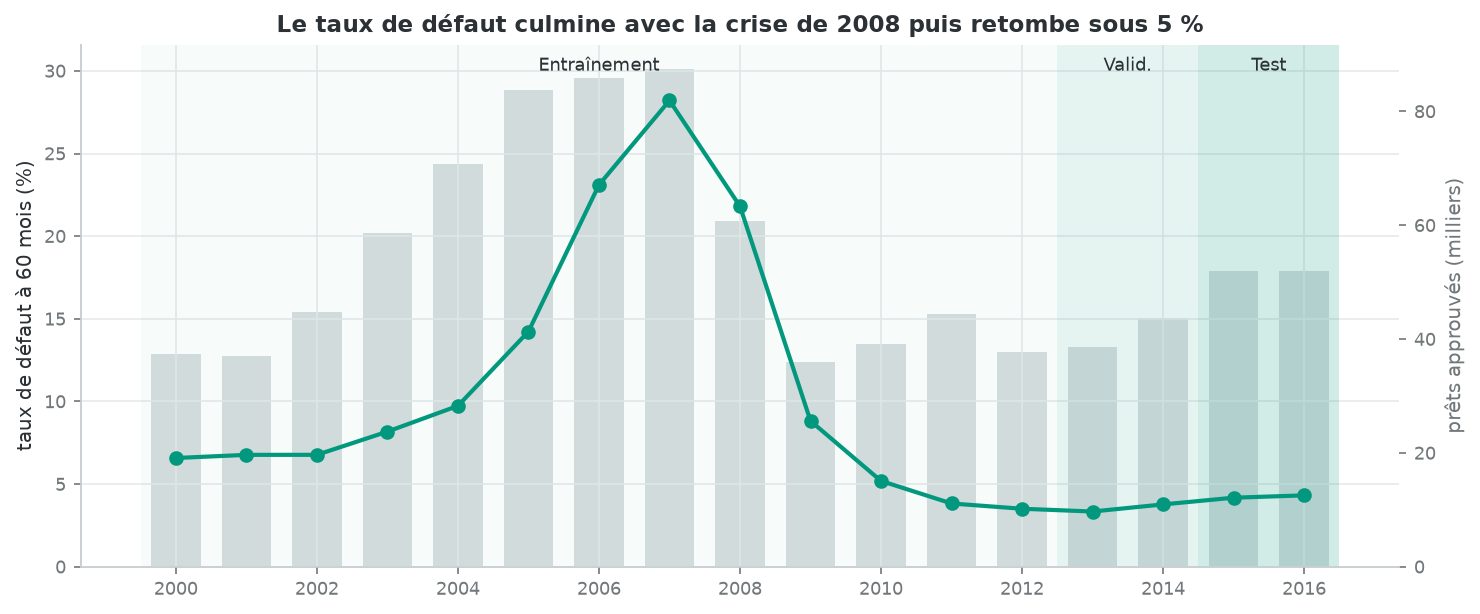
\includegraphics[width=\textwidth]{fig_defaut_par_annee.png}
  \caption{Taux de défaut à 60 mois (courbe) et nombre de prêts approuvés (barres) par année. Les zones colorées
  indiquent les blocs d'entraînement, de validation et de test.}
  \label{fig:annee}
\end{figure}

\subsection{Des classes déséquilibrées}

Le défaut est minoritaire dans les trois blocs (figure~\ref{fig:desequilibre}), de 3,6 à 13,5\,\% des prêts. Ce
déséquilibre justifie le choix de l'AUPRC et du score de Brier, en plus de l'AUROC, et un seuil de décision choisi sur
la validation plutôt que le seuil naïf de 0,5.

\begin{figure}[htbp]
  \centering
  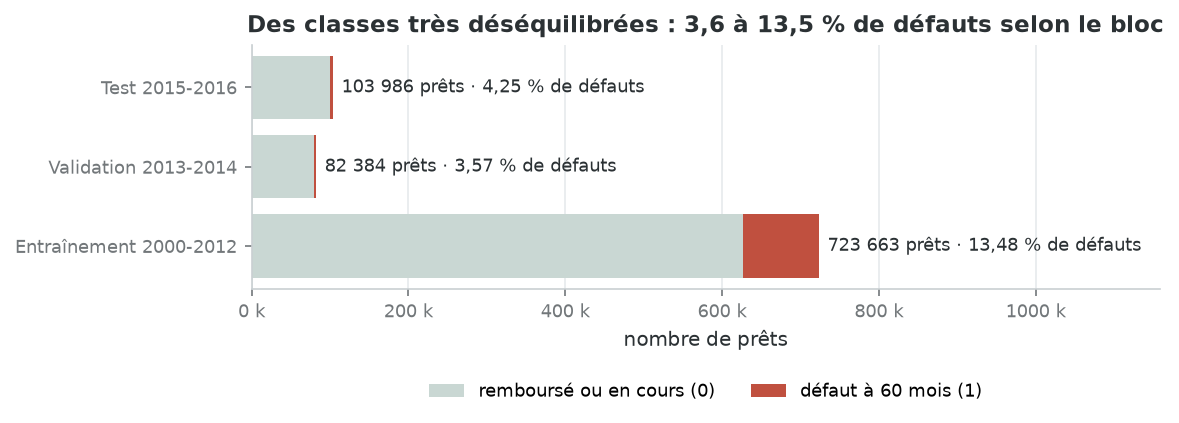
\includegraphics[width=0.85\textwidth]{fig_desequilibre.png}
  \caption{Répartition des prêts par issue dans chaque bloc.}
  \label{fig:desequilibre}
\end{figure}

\subsection{Secteur, montant et caractéristiques du prêt}

Le risque varie fortement selon le secteur (figure~\ref{fig:secteur}) : de 5,2\,\% dans l'agriculture à 19,0\,\% dans
l'immobilier, sur la période d'entraînement. Il décroît avec le montant (figure~\ref{fig:montant}) : les 10\,\% de
prêts les plus petits font défaut près de six fois plus souvent que les 10\,\% les plus gros (19,9\,\% contre
3,5\,\%). Les petits prêts, souvent accordés par des procédures simplifiées, sont octroyés à des entreprises plus
fragiles.

\begin{figure}[htbp]
  \centering
  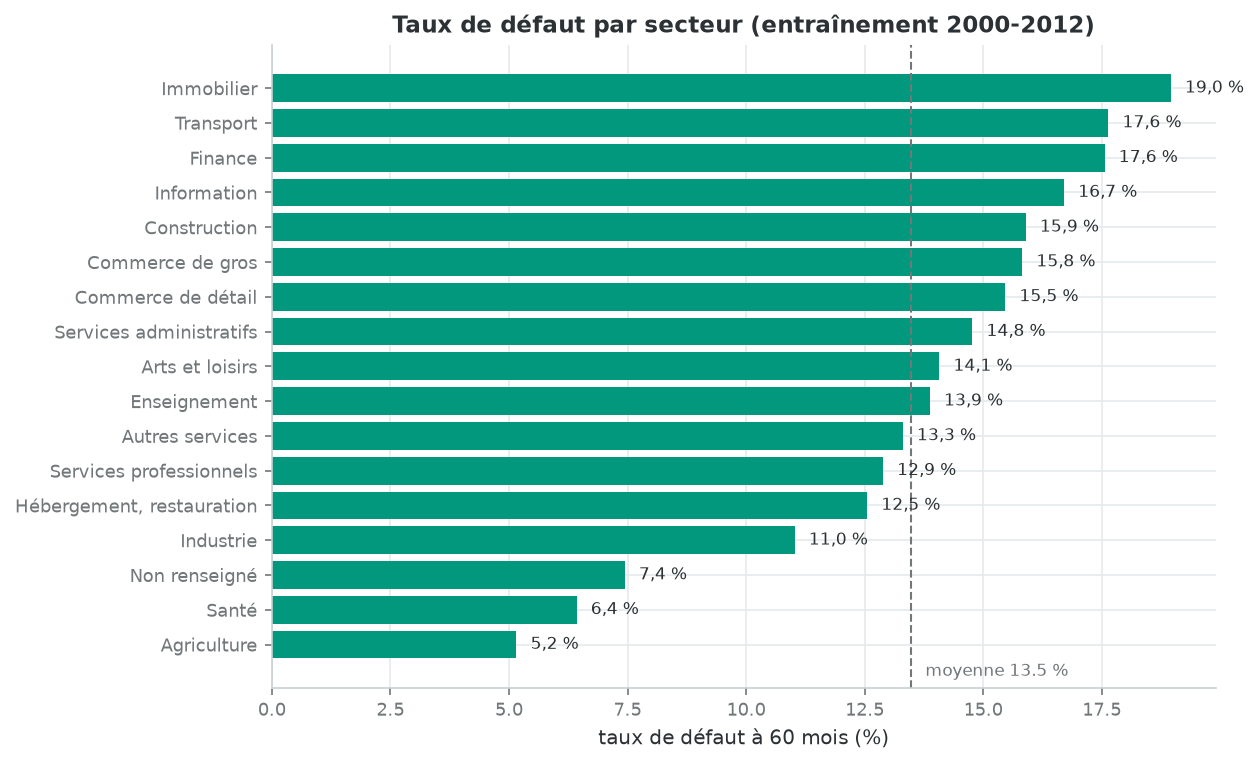
\includegraphics[width=0.8\textwidth]{fig_defaut_par_secteur.png}
  \caption{Taux de défaut par secteur d'activité (secteurs d'au moins 2\,000 prêts, entraînement). La ligne
  pointillée indique la moyenne.}
  \label{fig:secteur}
\end{figure}

\begin{figure}[htbp]
  \centering
  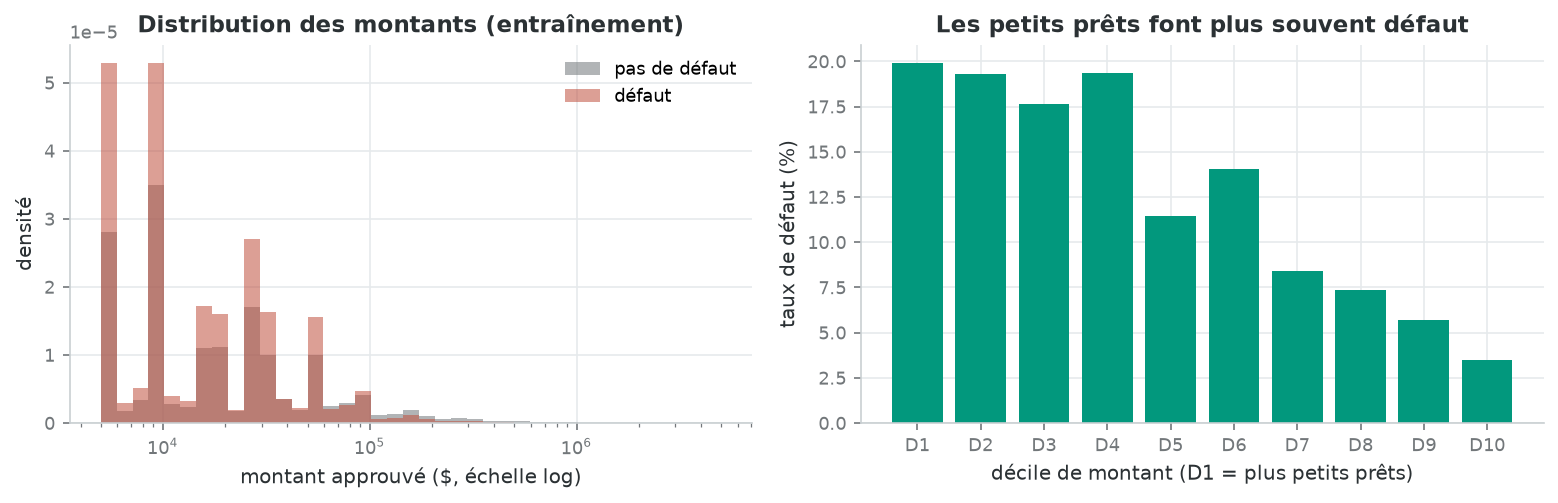
\includegraphics[width=\textwidth]{fig_montant.png}
  \caption{Distribution des montants selon l'issue (gauche) et taux de défaut par décile de montant (droite).
  Les pics de la distribution correspondent aux montants ronds (10\,000, 25\,000, 50\,000\,\$\dots).}
  \label{fig:montant}
\end{figure}

La figure~\ref{fig:categorielles} montre l'effet de quatre caractéristiques. La procédure d'octroi est la plus
discriminante : les programmes express (\textit{Community Express}, \textit{SBA Express}) ont des taux de défaut
deux à six fois plus élevés que les prêts instruits par des prêteurs certifiés. Les lignes de crédit renouvelables
sont plus risquées que les prêts amortissables. L'absence de taux d'intérêt renseigné est associée à un risque élevé,
mais c'est un artefact temporel : le taux n'est pas renseigné pour 79\,\% des prêts d'entraînement, surtout anciens
(figure~\ref{fig:manquants}), et il l'est pour tous les prêts de validation et de test.

\begin{figure}[htbp]
  \centering
  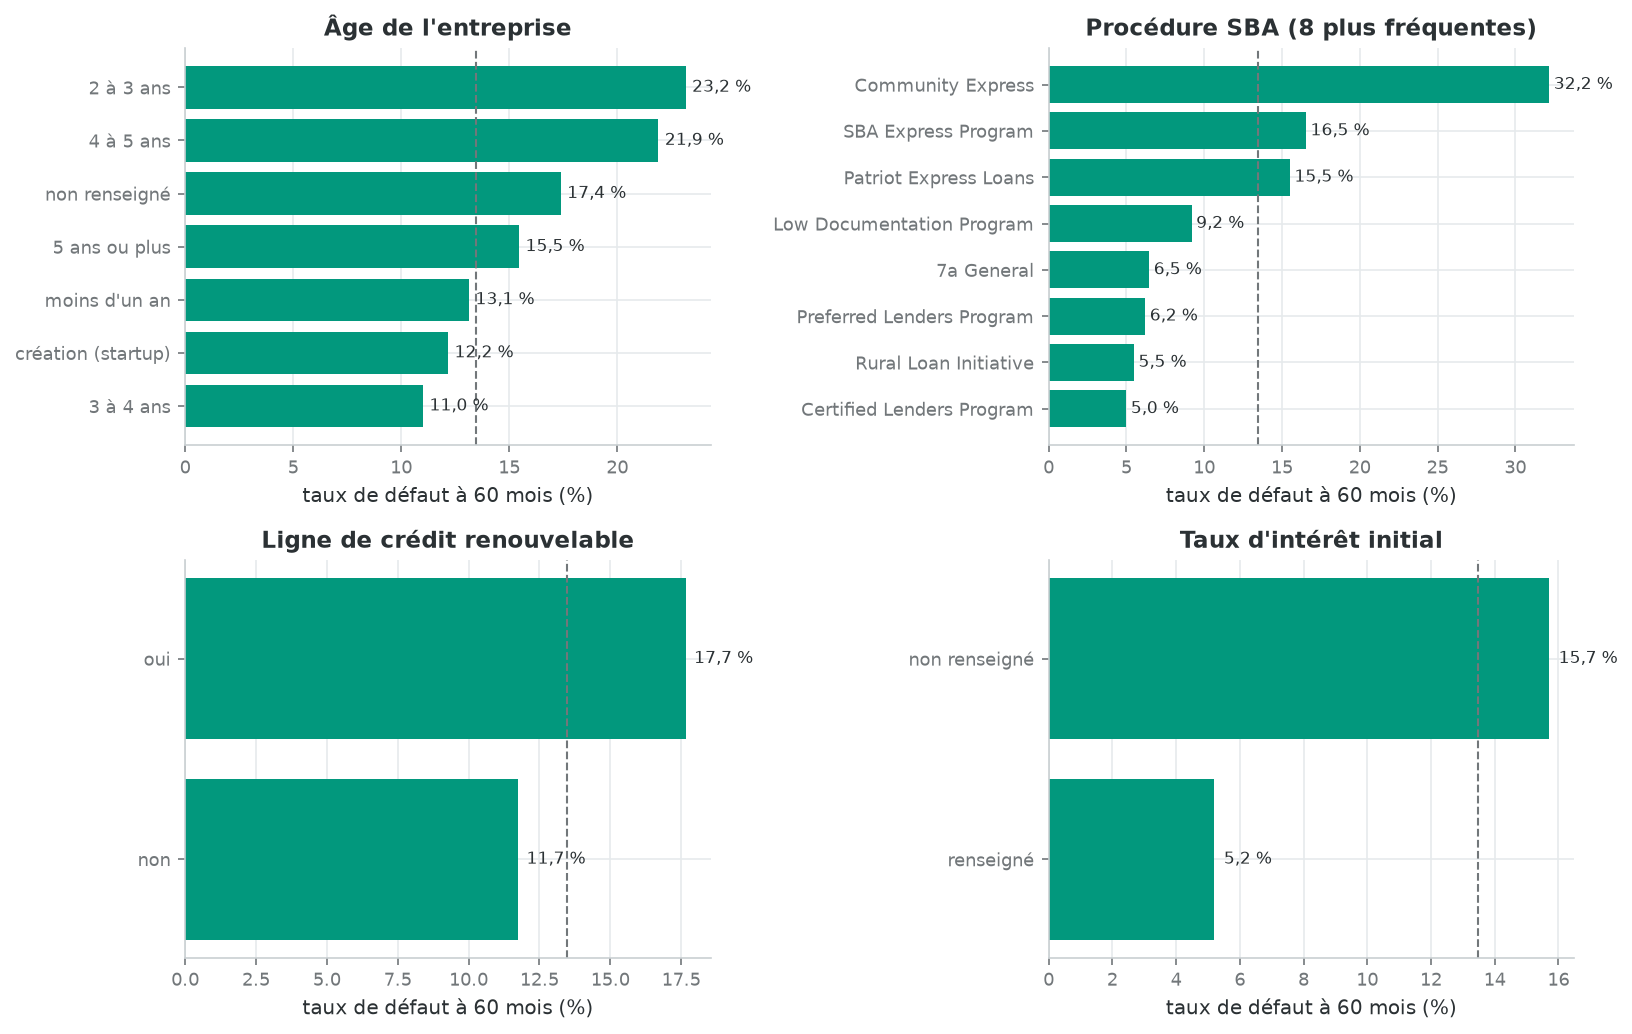
\includegraphics[width=\textwidth]{fig_variables_categorielles.png}
  \caption{Taux de défaut selon l'âge de l'entreprise, la procédure SBA, la ligne renouvelable et la présence du
  taux d'intérêt (entraînement ; ligne pointillée : moyenne).}
  \label{fig:categorielles}
\end{figure}

\begin{figure}[htbp]
  \centering
  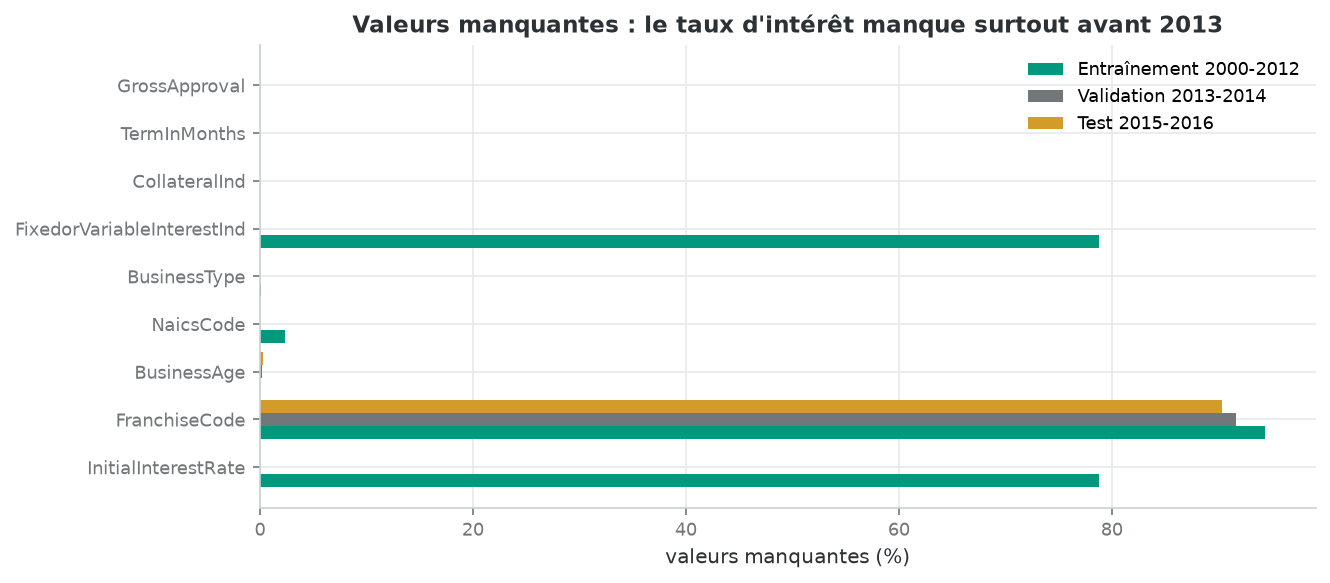
\includegraphics[width=0.85\textwidth]{fig_valeurs_manquantes.png}
  \caption{Part de valeurs manquantes par variable et par bloc. L'absence de code de franchise signifie
  \og pas de franchise \fg{} et n'est pas une donnée manquante.}
  \label{fig:manquants}
\end{figure}

\subsection{Une fuite de données détectée}\label{sec:fuite}

La durée du prêt est la variable la plus liée au défaut (figure~\ref{fig:duree}, gauche) : 28\,\% de défauts pour les
prêts de 60 mois ou moins, contre 2\,\% au-delà de 120 mois. Un premier modèle utilisant la durée exacte
(\code{TermInMonths}) atteignait une AUROC de 0,96 sur la validation, valeur trop élevée pour être crédible en
scoring de PME. L'examen de la variable a révélé la cause : les durées \og rondes \fg{} (12, 24, 60, 84, 120 mois)
correspondent à 1,6\,\% de défauts, les durées \og non rondes \fg{} (87, 129 mois\dots) à 34,9\,\%
(figure~\ref{fig:duree}, droite). La durée enregistrée est modifiée \emph{après} l'octroi lorsque le prêt tourne mal
(restructuration, résiliation) : elle contient en partie l'issue.

\begin{figure}[htbp]
  \centering
  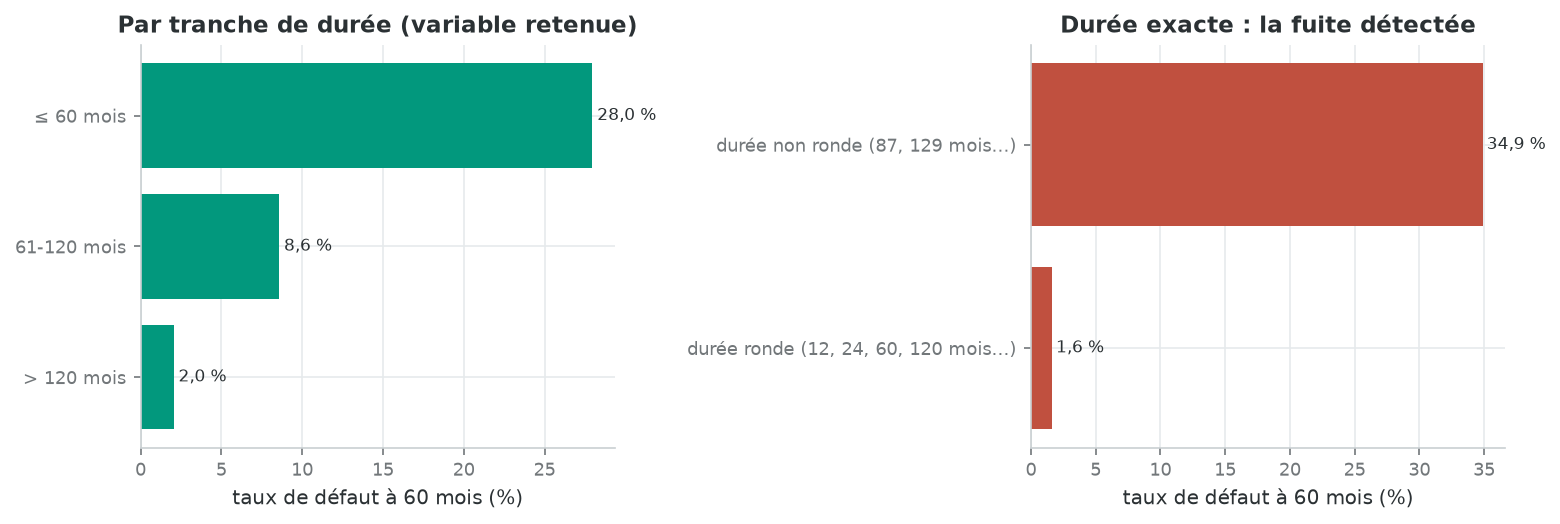
\includegraphics[width=\textwidth]{fig_duree.png}
  \caption{Taux de défaut par tranche de durée (gauche, variable retenue) et selon que la durée exacte est ronde ou
  non (droite) : la durée exacte révèle l'issue du prêt.}
  \label{fig:duree}
\end{figure}

\begin{encadre}[Correction retenue]
La durée exacte est remplacée par trois tranches larges : 60 mois ou moins, 61 à 120 mois, plus de 120 mois. Des tests
rapides donnaient une AUROC de validation de 0,96 avec la durée exacte, 0,81 avec cinq tranches, 0,79 avec trois
tranches et 0,67 sans aucune information de durée. Trois tranches conservent l'essentiel de l'information
légitime (un prêt court finance souvent un besoin plus risqué) sans laisser passer la fuite. C'est un écart assumé
par rapport à la liste de variables prévue initialement. La même vérification sur le taux d'intérêt n'a révélé
aucune anomalie.
\end{encadre}

% ---------------------------------------------------------------------------------------------
\section{Variables du modèle et prétraitement}

Les trois modèles utilisent exactement les mêmes 13 variables, toutes connues au moment de la demande
(tableau~\ref{tab:variables}).

\begin{table}[htbp]
\centering\small
\caption{Variables du modèle de risque}\label{tab:variables}
\begin{tabularx}{\textwidth}{>{\raggedright\arraybackslash}p{4cm}X}
\toprule
Variable & Construction \\
\midrule
Montant (log) & $\log(1 + \text{montant approuvé})$ \\
Part garantie & montant garanti par la SBA / montant approuvé \\
Taux d'intérêt initial & tel quel, avec une indicatrice \og taux non renseigné \fg{} \\
Tranche de durée & 3 tranches (section~\ref{sec:fuite}) \\
Taux fixe ou variable, ligne renouvelable & catégorielles \\
Secteur & deux premiers chiffres du code NAICS \\
État, type d'entreprise, âge de l'entreprise & catégorielles \\
Franchise & oui si un code de franchise est renseigné \\
Procédure SBA & catégorielle (express, prêteurs certifiés, etc.) \\
\bottomrule
\end{tabularx}
\end{table}

Deux variables disponibles sont volontairement exclues pour éviter un \emph{double comptage}. Le nombre d'emplois
soutenus devient le critère multicritère \og emplois par million \fg{}, et l'indicateur de garantie réelle sert au
critère \og couverture par les garanties \fg{}. Les garder dans le modèle ferait compter deux fois le même fait, une
fois dans la probabilité de défaut et une fois dans le critère.

Pour la régression logistique, les variables numériques sont imputées par la médiane puis standardisées, et les
catégorielles codées en indicatrices (les modalités rares, moins de 200 prêts, sont regroupées). Ces
transformations sont des \textit{pipelines} scikit-learn ajustés sur l'entraînement uniquement. L'EBM et LightGBM
traitent les variables catégorielles et les valeurs manquantes nativement ; pour LightGBM, les modalités sont
apprises sur l'entraînement et une modalité inconnue devient une valeur manquante.

% =============================================================================================
\chapter{Méthodologie et architecture}\label{chap:methodo}

% ---------------------------------------------------------------------------------------------
\section{Architecture du système}

La figure~\ref{fig:chaine} présente la chaîne de décision. À gauche, les données réelles et le modèle de risque ;
à droite, les paramètres sectoriels et la simulation ; les deux se rejoignent dans une table de huit critères par
projet, qui alimente le filtre, la méthode multicritère, l'arbitrage budgétaire et les agents de rédaction, avant la
décision humaine.

\begin{figure}[htbp]
\centering
\begin{tikzpicture}[
  font=\small,
  box/.style={draw=eccgris,rounded corners=3pt,align=center,minimum height=1.05cm,text width=5.6cm,fill=white},
  key/.style={box,draw=eccvert,line width=1pt,fill=eccclair},
  arr/.style={-{Stealth[length=2.2mm]},eccgris,thick},
  node distance=0.55cm]
  \node[box] (sba) {\textbf{Données SBA 7(a)}\\ 910\,033 prêts réels, 2000-2016};
  \node[box,right=0.9cm of sba] (dam) {\textbf{Paramètres Damodaran}\\ coût du capital, dette, par secteur};
  \node[box,below=of sba] (ml) {\textbf{Modèle de risque}\\ EBM calibré : probabilité de défaut};
  \node[box,below=of dam] (sim) {\textbf{Simulation des 40 projets}\\ VAN, délai, DSCR, levier, garanties, ESG};
  \coordinate (milieu) at ($(ml.south)!0.5!(sim.south)$);
  \node[box,below=0.55cm of milieu,text width=12.2cm] (scores) {\textbf{Table des critères}\\
        8 critères pour chacun des 40 projets (risque issu du ML + 7 indicateurs)};
  \node[box,below=of scores,text width=12.2cm] (filtre) {\textbf{Agent de conformité : filtre éliminatoire}\\
        DSCR $< 1$ ou probabilité de défaut $> 7{,}1\,\%$ : Refuser};
  \node[key,below=of filtre,text width=12.2cm] (mcda) {\textbf{Moteur MCDA (déterministe)}\\
        poids AHP ; ELECTRE III (classement) ; ELECTRE TRI (catégorie) ; PROMETHEE II (vérification)};
  \node[box,below=of mcda,xshift=-3.3cm,text width=5.6cm] (rob) {\textbf{Agent de robustesse}\\
        200 scénarios de paramètres, 20 tirages};
  \node[box,below=of mcda,xshift=3.3cm,text width=5.6cm] (arb) {\textbf{Agent d'arbitrage}\\
        budget, bornes, plafond sectoriel};
  \node[box,below=2.2cm of mcda,text width=12.2cm] (llm) {\textbf{Agents fondés sur un LLM}\\
        agent rédacteur (note par projet) et conseiller (questions, outils) ; aucun calcul};
  \node[key,below=of llm,text width=7cm] (comite) {\textbf{Comité d'investissement}\\ fixe les paramètres, décide};
  \draw[arr] (sba) -- (ml);
  \draw[arr] (dam) -- (sim);
  \draw[arr,dashed] (sba.east) -- ++(0.45,0) |- node[pos=0.25,right,font=\scriptsize,text=eccgris]{40 prêts du test} (sim.west);
  \draw[arr] (ml) -- (ml|-scores.north);
  \draw[arr] (sim) -- (sim|-scores.north);
  \draw[arr] (scores) -- (filtre);
  \draw[arr] (filtre) -- (mcda);
  \draw[arr] (mcda.south-|rob.north) -- (rob);
  \draw[arr] (mcda.south-|arb.north) -- (arb);
  \draw[arr] (rob) -- (rob|-llm.north);
  \draw[arr] (arb) -- (arb|-llm.north);
  \draw[arr] (llm) -- (comite);
\end{tikzpicture}
\caption{Chaîne de décision : le ML estime le risque, le MCDA classe et catégorise, l'arbitrage respecte le budget,
les agents LLM rédigent, le comité décide.}
\label{fig:chaine}
\end{figure}

\subsection{De l'architecture proposée à l'architecture réalisée}

Le sujet proposait une architecture à neuf composantes. Le tableau~\ref{tab:archi} indique, pour chacune, ce qui a
été réalisé et les écarts. Conformément au sujet, le moteur MCDA est un outil déterministe et non un agent : seuls
la rédaction et le dialogue reposent sur un modèle de langage.

\begin{table}[htbp]
\centering\footnotesize
\caption{Architecture proposée par le sujet et réalisation}\label{tab:archi}
\begin{tabularx}{\textwidth}{>{\raggedright\arraybackslash}p{3.4cm}X>{\raggedright\arraybackslash}p{2.1cm}}
\toprule
Composante proposée & Réalisation dans le projet & Statut \\
\midrule
1. Agent extracteur (lecture de dossiers) & Non réalisé : nos dossiers sont des données structurées. L'import d'un
fichier CSV ou Excel et le calcul automatique de la probabilité de défaut jouent ce rôle. & Écart assumé \\
2. Agent de conformité & Filtre éliminatoire à règles (DSCR, risque), configurable. & Réalisé \\
3. Agents d'analyse par dimension & Modèle de risque (EBM) et facteurs de risque par projet ; VAN, délai et DSCR
calculés par la simulation. Le TRI et la détection d'anomalies ne sont pas calculés. & Réalisé en partie \\
4. Validation par les analystes & Page de configuration : critères, poids, jugements AHP, profils et filtre
modifiables avant le calcul. & Réalisé \\
5. Moteur MCDA & AHP, ELECTRE III, ELECTRE TRI, PROMETHEE II, implémentés en Python et testés à la main. & Réalisé \\
6. Agent d'arbitrage & Sélection sous budget, bornes de montant et plafond sectoriel (deux règles). & Réalisé \\
7. Agent de robustesse & 200 scénarios de paramètres, 20 tirages de simulation, scénarios « et si » du conseiller. &
Réalisé \\
8. Agent rédacteur & Note par projet par LLM, avec vérification des nombres et note de repli sans LLM. & Réalisé \\
9. Comité d'investissement & Paramètres fixés en amont dans la configuration ; décision humaine en aval. & Réalisé \\
\bottomrule
\end{tabularx}
\end{table}

% ---------------------------------------------------------------------------------------------
\section{Modèle de risque}

\subsection{Protocole}

\begin{enumerate}
  \item Les trois modèles sont entraînés sur 2000-2012 avec les mêmes 13 variables.
  \item Leurs hyperparamètres sont choisis sur l'AUROC de validation, par une grille volontairement courte
        (tableau~\ref{tab:hyper}) : quatre valeurs de $C$ pour la logistique, deux nombres d'interactions pour l'EBM,
        deux nombres de feuilles pour LightGBM, dont le nombre d'arbres est fixé par arrêt anticipé (100 tours sans
        amélioration).
  \item Chaque modèle est calibré par régression isotonique ajustée sur la validation. Pour mesurer honnêtement la
        calibration sur la validation elle-même, on utilise une calibration croisée en cinq blocs.
  \item Le seuil F1 est choisi sur la validation.
  \item Le modèle retenu est choisi sur la validation, selon une règle fixée \emph{avant} d'entraîner LightGBM.
  \item Le test (2015-2016) est lu une seule fois, après le choix, pour les métriques finales.
\end{enumerate}

\begin{table}[htbp]
\centering
\footnotesize\setlength{\tabcolsep}{4pt}
\caption{Réglage des hyperparamètres sur la validation}\label{tab:hyper}
\begin{tabular}{lllrc}
\toprule
Modèle & Hyperparamètres & AUROC val. (brut) & Durée (s) & Retenu \\
\midrule
Logistique & C=0.01 & 0,7348 & 20 & oui \\
Logistique & C=0.1 & 0,7308 & 26 &  \\
Logistique & C=1 & 0,7297 & 26 &  \\
Logistique & C=10 & 0,7293 & 30 &  \\
EBM & interactions=3, taux d'apprentissage=0.05 & 0,7676 & 191 &  \\
EBM & interactions=10, taux d'apprentissage=0.05 & 0,7692 & 279 & oui \\
LightGBM & feuilles=31, arbres=334 & 0,7933 & 18 &  \\
LightGBM & feuilles=127, arbres=147 & 0,7959 & 17 & oui \\
\bottomrule
\end{tabular}
\end{table}


\subsection{Règle de choix du modèle}

\begin{encadre}[Règle de choix]
Le modèle utilisé est celui dont le score de Brier calibré est le plus bas sur la validation, \textbf{parmi les
modèles interprétables} (régression logistique et EBM). Le Brier est retenu parce que le MCDA utilise la valeur de la
probabilité ; l'interprétabilité est exigée parce qu'une banque doit pouvoir expliquer un refus de crédit.
LightGBM n'est pas candidat : il sert d'étalon pour mesurer ce que coûte l'interprétabilité.
\end{encadre}

% ---------------------------------------------------------------------------------------------
\section{Simulation des 40 projets candidats}\label{sec:simulation}

\subsection{Principe}

Les 40 projets sont de vrais prêts tirés au hasard dans le bloc de test (graine fixe 2026), que le modèle n'a jamais
vus. Leur probabilité de défaut est celle du modèle ; leurs indicateurs financiers sont simulés. La vraie issue du
prêt est retirée du tableau avant le tirage, si bien que la simulation ne peut pas l'utiliser. Le nombre de 40 permet
de voir l'effet du veto ($40 \times 39 = 1\,560$ comparaisons) tout en restant lisible.

\subsection{Étapes}

\begin{enumerate}
  \item \textbf{Secteur} : chaque code NAICS à deux chiffres est rattaché à un secteur de Damodaran par une table
        faite à la main (tableau~\ref{tab:damodaran} en annexe) ; les cas flous prennent la moyenne du marché.
  \item \textbf{Paramètres} : le taux d'actualisation est le coût du capital du secteur, tiré à $\pm$\,20\,\% ; la
        croissance des flux est une hypothèse d'équipe par secteur, elle aussi tirée à $\pm$\,20\,\%.
  \item \textbf{Financement} : la dette représente entre 50 et 80\,\% de l'investissement ; le levier dette sur fonds
        propres est donc compris entre 1 et 4.
  \item \textbf{DSCR piloté} : 8 projets \og faibles \fg{} (DSCR minimum tiré entre 0,8 et 1,0), 24 \og moyens \fg{}
        (1,0 à 1,5) et 8 \og solides \fg{} (1,5 à 2,0), soit 20\,/\,60\,/\,20\,\%. Les flux annuels croissent avec un
        bruit de 5\,\%, puis sont mis à l'échelle pour que le pire DSCR tombe exactement sur la valeur tirée.
  \item \textbf{VAN et délai} : dix années de flux explicites, une valeur résiduelle en perpétuité sans croissance
        réduite de moitié par prudence ; la durée du prêt est la durée standard de sa tranche (5, 10 ou 25 ans).
  \item \textbf{Garanties} : couverture nulle si le prêt réel n'avait pas de garantie, sinon tirée entre 0,5 et 1,5.
  \item \textbf{ESG} : une classe A, B ou C tirée selon le groupe de secteurs (industrie plutôt A ou B, services plutôt
        C), puis une note autour de 30, 60 ou 85 avec un bruit de 5 points.
  \item \textbf{Emplois par million} : nombre réel d'emplois soutenus divisé par le montant en millions de dollars.
\end{enumerate}

\begin{encadre}[Ce qui est sourcé et ce qui est un choix]
Le coût du capital (Damodaran) et les repères de DSCR (1,25 ; 1,3 à 1,4 dans l'énergie~\cite{nrel2024}) sont
sourcés. Les autres paramètres (croissance, horizon, décote de la valeur résiduelle, bruit, bornes de dette et de
garantie, centres ESG, durées standard) sont des hypothèses d'équipe, testées en sensibilité. Chaque projet reçoit
enfin un nom lisible et fictif (« Cabinet dentaire Baker ») : l'activité vient du vrai code NAICS, le nom de famille
d'une liste fixe ; aucun vrai nom d'emprunteur n'est utilisé.
\end{encadre}

% ---------------------------------------------------------------------------------------------
\section{Paramétrage de la méthode multicritère}

\subsection{Critères, poids et profils}

Le tableau~\ref{tab:criteres} donne les huit critères, leur sens, leurs poids et les profils d'ELECTRE TRI. Les poids
cibles traduisent l'ordre de priorité d'une banque : d'abord le remboursement (risque, DSCR), puis la rentabilité,
puis la protection (garanties, levier), enfin l'impact (ESG, emplois). Les 28 jugements de l'AHP
(tableau~\ref{tab:ahp} en annexe) ont été initialisés en arrondissant à l'échelle de Saaty les rapports de ces poids
cibles ; ils sont modifiables dans l'application.

\begin{table}[htbp]
\centering
\footnotesize\setlength{\tabcolsep}{4pt}
\caption{Critères, poids AHP et profils ELECTRE TRI ($b_1$ : Refuser $|$ Conditionner ; $b_2$ : Conditionner $|$ Financer)}\label{tab:criteres}
\begin{tabular}{lcccccl}
\toprule
Critère & Sens & Poids cible & Poids AHP & Profil $b_1$ & Profil $b_2$ & Type \\
\midrule
Probabilité de défaut & min & 25\,\% & 25,8\,\% & 5,4\,\% & 3,6\,\% & absolu \\
VAN & max & 15\,\% & 16,1\,\% & 0\,\$ & 85\,353\,\$ & mixte \\
Délai de récupération & min & 8\,\% & 8,2\,\% & 10,0\,ans & 6,5\,ans & mixte \\
DSCR minimum & max & 20\,\% & 20,1\,\% & 1,00 & 1,25 & absolu \\
Dette / fonds propres & min & 10\,\% & 9,4\,\% & 3,00 & 1,50 & absolu \\
Couverture par les garanties & max & 10\,\% & 9,4\,\% & 0,50 & 1,00 & absolu \\
Score ESG & max & 7\,\% & 6,2\,\% & 50 & 70 & absolu \\
Emplois par million \$ & max & 5\,\% & 5,0\,\% & 15,63 & 54,00 & relatif \\
\bottomrule
\end{tabular}
\end{table}


Les profils sont \emph{absolus} lorsqu'un repère existe (probabilité de défaut rapportée au taux de référence,
DSCR de 1 et 1,25, levier, garanties couvrant la moitié puis la totalité du prêt, ESG), afin qu'une catégorie traduise
un standard de crédit plutôt qu'un rang dans le lot. Ils sont relatifs (tertiles du lot) quand aucun repère externe
n'existe.

\subsection{Filtre éliminatoire}

Avant le classement, un projet est écarté si son DSCR minimum est inférieur à 1 ou si sa probabilité de défaut dépasse
deux fois le taux de défaut de référence. Le veto d'ELECTRE est relatif (il empêche $a$ de surclasser $b$ si $b$ est
bien meilleur sur un critère) et n'élimine pas un projet dans l'absolu : un seuil absolu doit donc être un filtre.

\begin{encadre}[Adaptation du taux de référence]
La règle prévoyait \og 2 fois le taux de défaut moyen de l'entraînement \fg{}, soit $2 \times 13{,}48\,\% = 27\,\%$.
Or la probabilité de défaut est calibrée sur 2013-2014 : aucun des 40 projets ne dépasse 18\,\%, et le filtre ne se
déclenchait jamais. Comparer une probabilité d'une période à un taux d'une autre période étant incohérent, le taux de
référence retenu est celui de la validation (3,57\,\%), soit un seuil de 7,1\,\%.
\end{encadre}

\subsection{Seuils, coupure et robustesse}

Les seuils d'ELECTRE III et de PROMETHEE II sont exprimés en pourcentage de l'étendue observée de chaque critère :
$q = 5\,\%$, $p = 20\,\%$, $v = 50\,\%$. La coupure d'ELECTRE TRI vaut $\lambda = 0{,}6$ et la règle d'affectation est
pessimiste. La robustesse est mesurée de trois façons : un paramètre à la fois (quatre jeux de seuils, six valeurs de
$\lambda$) ; 200 scénarios combinés tirant les poids à $\pm$\,30\,\%, les seuils dans les plages testées et $\lambda$
entre 0,5 et 0,8 (une décision est \og fragile \fg{} si sa catégorie change dans au moins 25\,\% des scénarios) ;
et 20 nouveaux tirages des indicateurs simulés pour les mêmes 40 prêts.

% ---------------------------------------------------------------------------------------------
\section{Agent d'arbitrage}

L'arbitrage reçoit les catégories du MCDA et choisit les projets à financer sous un budget global, des montants
minimum et maximum par projet et une part maximale par secteur. Pour la démonstration : budget de 5\,M\$, montants
de 20\,000\,\$ à 2\,M\$ et 35\,\% du budget au plus par secteur. Les projets \og Financer \fg{} passent d'abord, puis,
si on l'autorise, les projets \og sous conditions \fg{}. Deux règles sont proposées (section~\ref{sec:theorie-budget}) :

\begin{itemize}
  \item \textbf{suivre le classement} (règle par défaut) : on parcourt les projets dans l'ordre de priorité du comité
        (catégorie, puis rang ELECTRE III) et l'on retient chacun s'il respecte encore les trois contraintes. C'est
        l'optimum exact lorsque tout projet mieux classé doit passer avant les autres, et chaque projet écarté reçoit
        un motif précis ;
  \item \textbf{maximiser le nombre} : programme linéaire en nombres entiers qui retient le plus de projets
        \og Financer \fg{}, puis \og sous conditions \fg{}, puis, à nombre égal, les mieux classés.
\end{itemize}

% ---------------------------------------------------------------------------------------------
\section{Agents fondés sur un modèle de langage}

\subsection{Agent rédacteur}

Pour chaque projet, Python rassemble les \og faits \fg{} déjà calculés et formatés : catégorie, rangs, huit critères,
motif d'exclusion, fragilité, facteurs de risque, statut budgétaire. Le LLM reçoit ces faits avec la consigne de les
recopier sans en créer et rédige une note de six à neuf phrases pour le comité. Un vérificateur extrait tous les nombres
de la note : si un seul n'appartient pas aux faits, la note est rejetée et remplacée par une note de gabarit, écrite
sans LLM.

\subsection{Conseiller conversationnel}

Le conseiller répond en français aux questions sur les projets, les résultats, des scénarios et la méthode. Il ne voit
pas les données : il dispose de dix outils, des fonctions Python déterministes décrites par un schéma
(tableau~\ref{tab:outils}), et rédige à partir de leurs résultats. Sous chaque réponse, l'utilisateur voit les outils
appelés et leurs résultats bruts.

\begin{table}[htbp]
\centering\footnotesize
\caption{Outils du conseiller}\label{tab:outils}
\begin{tabularx}{\textwidth}{>{\ttfamily}p{3.6cm}X}
\toprule
\normalfont Outil & Rôle \\
\midrule
capacites & ce que le conseiller sait faire, ses limites et les méthodes réellement utilisées \\
resume\_resultats & vue d'ensemble : catégories, exclusions, poids, meilleurs projets, fragilité \\
lister\_projets & liste filtrée et triée (catégorie, texte, critère) \\
fiche\_projet & tous les faits d'un projet, éventuellement sous un scénario de poids, de coupure ou sans filtre \\
comparer\_projets & deux à six projets critère par critère \\
statistiques & moyenne, médiane, minimum, maximum d'un critère, par groupe \\
simuler\_scenario & relance le MCDA avec d'autres poids, une autre coupure ou sans filtre \\
arbitrage\_budget & sélection sous budget, avec simulation d'un autre budget \\
parametres\_methode & paramètres réels et explication de la méthode \\
donnees\_historiques & données SBA : taux de défaut, audit, métriques et erreurs du modèle \\
\bottomrule
\end{tabularx}
\end{table}

Deux contrôles automatiques complètent l'appel d'outils. Chaque nombre de la réponse doit figurer dans les résultats
des outils consultés, sinon un avertissement s'affiche. Toute méthode citée mais non utilisée (par exemple une variante
d'ELECTRE inventée par le modèle) déclenche aussi un avertissement. Le fournisseur est Google Gemini, dans son offre
gratuite ; l'application bascule automatiquement sur d'autres modèles en cas de saturation, et fonctionne sans LLM
(notes de gabarit, questions rapides) si aucune clé n'est configurée.

% =============================================================================================
\chapter{Résultats}\label{chap:resultats}

% ---------------------------------------------------------------------------------------------
\section{Modèle de risque}

\subsection{Comparaison des trois modèles}

Le tableau~\ref{tab:modeles} donne les performances des versions calibrées. Sur le test, lu une seule fois, LightGBM
obtient la meilleure AUROC (0,800), devant l'EBM (0,778) et la régression logistique (0,726). Le même ordre se retrouve
en AUPRC (0,200, 0,170 et 0,159, pour un taux de défaut de 4,25\,\%, donc environ quatre à cinq fois mieux que le
hasard) et en F1.

\begin{table}[htbp]
\centering
\footnotesize\setlength{\tabcolsep}{4pt}
\caption{Performances des trois modèles (versions calibrées). Taux de défaut réel : 3,57\,\% en validation, 4,25\,\% en test}\label{tab:modeles}
\begin{tabular}{lccccccc}
\toprule
Modèle (calibré) & AUROC val. & Brier val. & AUROC test & AUPRC test & F1 test & Brier test & PD moy. test \\
\midrule
Régression logistique & 0,733 & 0,0325 & 0,726 & 0,159 & 0,239 & 0,0380 & 3,67\,\% \\
\textbf{EBM (retenu)} & 0,767 & 0,0325 & 0,778 & 0,170 & 0,247 & 0,0379 & 3,52\,\% \\
LightGBM (référence) & 0,793 & 0,0318 & 0,800 & 0,200 & 0,282 & 0,0370 & 3,59\,\% \\
\bottomrule
\end{tabular}
\end{table}


\begin{encadre}[Le prix de l'interprétabilité]
La règle de choix, fixée avant l'entraînement de LightGBM, retient l'\textbf{EBM}, meilleur modèle interprétable sur
la validation (Brier calibré de 0,03248 contre 0,03249 pour la logistique, et une AUROC nettement supérieure). L'écart
entre l'EBM et LightGBM sur le test est de 0,022 point d'AUROC et 0,030 point d'AUPRC, alors que l'EBM dépasse la
baseline de 0,052 point d'AUROC. Autrement dit, le modèle interprétable récupère environ 70\,\% du gain apporté par le
modèle opaque par rapport à la baseline. Pour une décision de crédit qui doit être justifiée, ce prix est faible.
\end{encadre}

\subsection{Calibration}

La figure~\ref{fig:calibration} compare les courbes de calibration. Sur la validation, les trois modèles calibrés
suivent la diagonale, ce qui est attendu puisque la calibration y est ajustée (de façon croisée pour la mesure). Sur
le test, les courbes restent proches de la diagonale pour les probabilités inférieures à 5\,\%, où se trouvent la
plupart des prêts, mais passent au-dessus pour les risques les plus élevés : les modèles sous-estiment le risque des
prêts les plus fragiles de 2015-2016. En moyenne, l'EBM prédit 3,52\,\% de défauts pour un taux réel de 4,25\,\%. Ce
léger décalage reflète la dérive entre périodes (le taux de défaut remonte de 3,6 à 4,3\,\% entre la validation et le
test) ; il conduit à une estimation un peu optimiste du risque, à garder à l'esprit dans l'interprétation.

\begin{figure}[htbp]
  \centering
  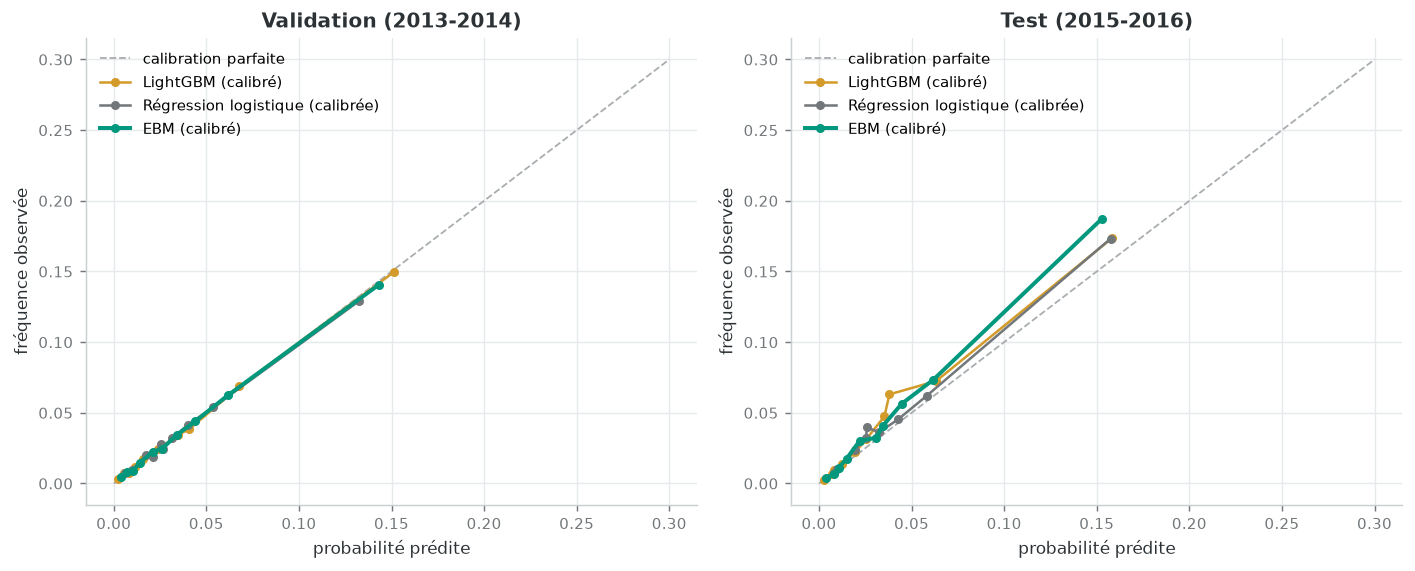
\includegraphics[width=\textwidth]{calibration.png}
  \caption{Courbes de calibration des trois modèles calibrés, sur la validation et sur le test (déciles de
  probabilité prédite).}
  \label{fig:calibration}
\end{figure}

\subsection{Interprétabilité}

\paragraph{Importance des variables.} L'importance par permutation de l'EBM et les valeurs SHAP de LightGBM
(tableau~\ref{tab:importance}, figures~\ref{fig:importance} et~\ref{fig:shap}) désignent les mêmes variables
principales : la tranche de durée et le taux d'intérêt initial, puis le montant, la procédure, l'État et la ligne
renouvelable. Mélanger la tranche de durée fait perdre 0,189 point d'AUROC à l'EBM, dix fois plus que toute autre
variable. Deux modèles de natures différentes s'accordant sur les facteurs de risque, ces résultats sont robustes.

\begin{table}[htbp]
\centering
\footnotesize\setlength{\tabcolsep}{4pt}
\caption{Importance des variables sur la validation : permutation pour l'EBM, valeurs SHAP pour LightGBM}\label{tab:importance}
\begin{tabular}{lccc}
\toprule
Variable & Baisse d'AUROC (EBM) & Écart-type & $|$SHAP$|$ moyen (LightGBM) \\
\midrule
tranche de durée & 0,1887 & 0,0080 & 0,723 \\
taux d'intérêt initial & 0,0295 & 0,0027 & 0,809 \\
montant (log) & 0,0270 & 0,0038 & 0,146 \\
ligne renouvelable & 0,0229 & 0,0017 & 0,069 \\
procédure SBA & 0,0170 & 0,0007 & 0,150 \\
État & 0,0116 & 0,0022 & 0,208 \\
taux fixe ou variable & 0,0088 & 0,0011 & 0,100 \\
secteur NAICS & 0,0084 & 0,0013 & 0,174 \\
part garantie SBA & 0,0028 & 0,0009 & 0,076 \\
type d'entreprise & 0,0005 & 0,0005 & 0,022 \\
franchise & 0,0001 & 0,0002 & 0,004 \\
taux non renseigné & 0,0000 & 0,0000 & 0,164 \\
âge de l'entreprise & -0,0002 & 0,0011 & 0,120 \\
\bottomrule
\end{tabular}
\end{table}


\begin{figure}[htbp]
  \centering
  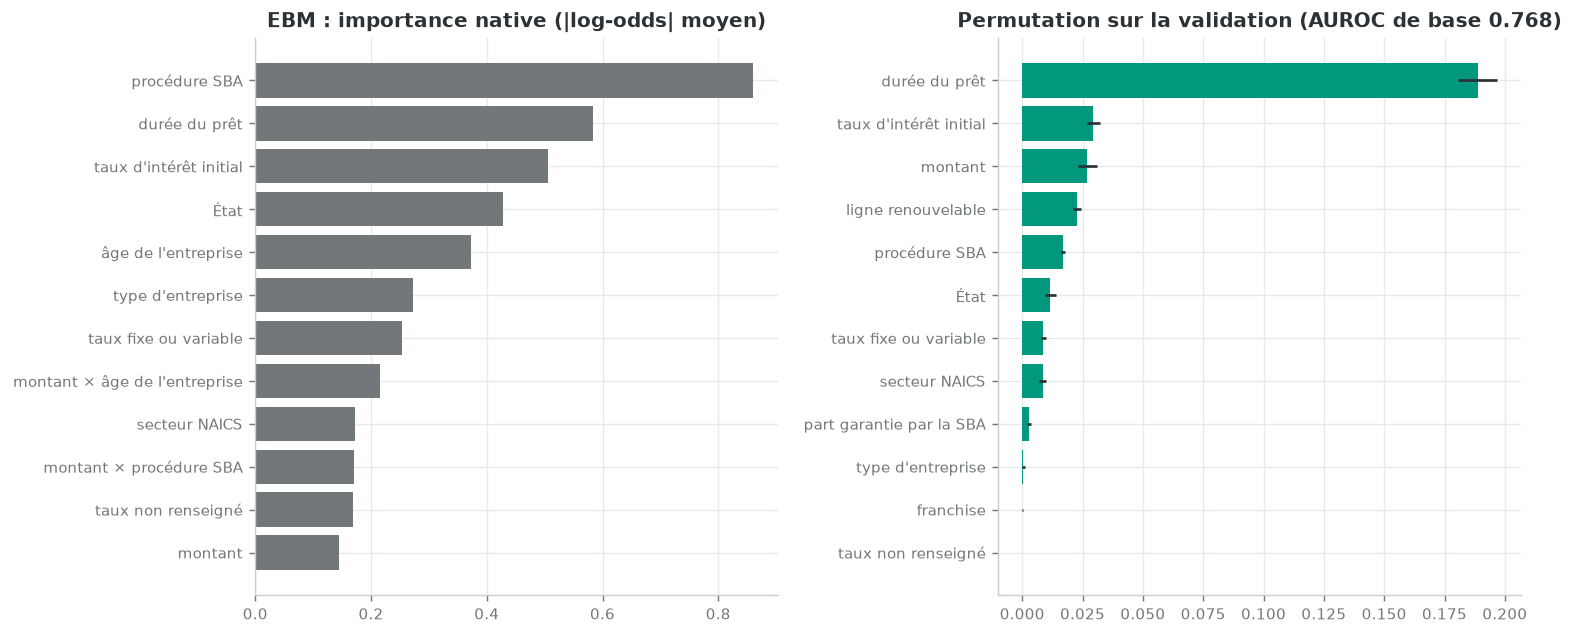
\includegraphics[width=\textwidth]{importance_variables.png}
  \caption{Importance native de l'EBM (contribution absolue moyenne, à gauche) et importance par permutation sur la
  validation (baisse d'AUROC, à droite).}
  \label{fig:importance}
\end{figure}

\begin{figure}[htbp]
  \centering
  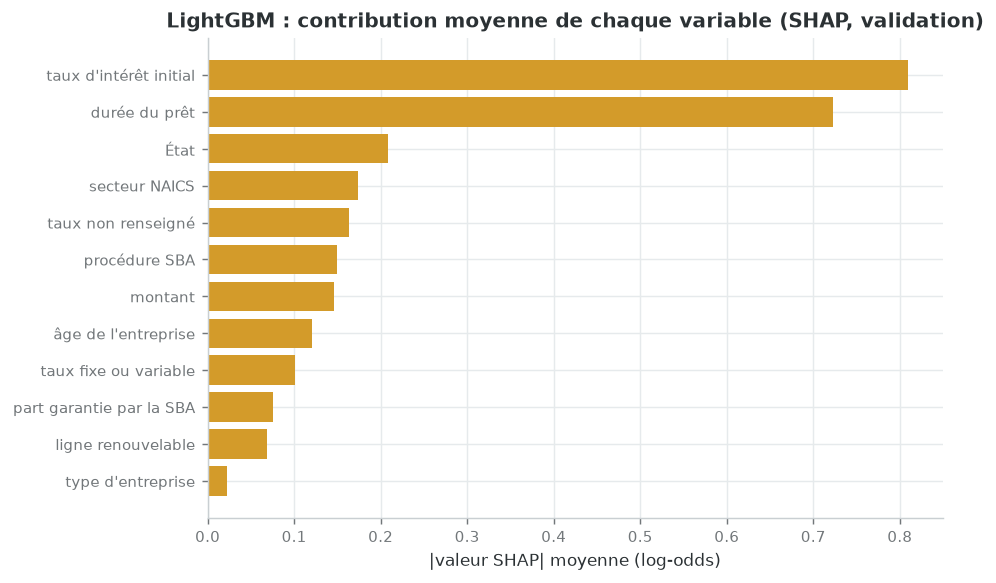
\includegraphics[width=0.75\textwidth]{shap_lightgbm.png}
  \caption{LightGBM : valeur SHAP absolue moyenne par variable (5\,000 prêts de validation).}
  \label{fig:shap}
\end{figure}

\paragraph{Effet des variables.} La figure~\ref{fig:effets} montre les fonctions apprises par l'EBM pour ses quatre
variables principales. Les prêts courts (60 mois ou moins) augmentent nettement le risque, les prêts longs le
réduisent. Les procédures express (\textit{Community Express}, \textit{Patriot Express}) l'augmentent, les prêteurs
certifiés le réduisent. L'effet du taux initial est en U : les taux très bas (souvent des prêts anciens ou
particuliers) comme les taux élevés (emprunteurs jugés risqués par la banque prêteuse) sont associés à plus de
défauts. Ces effets sont cohérents avec l'analyse exploratoire et avec l'intuition bancaire.

\begin{figure}[htbp]
  \centering
  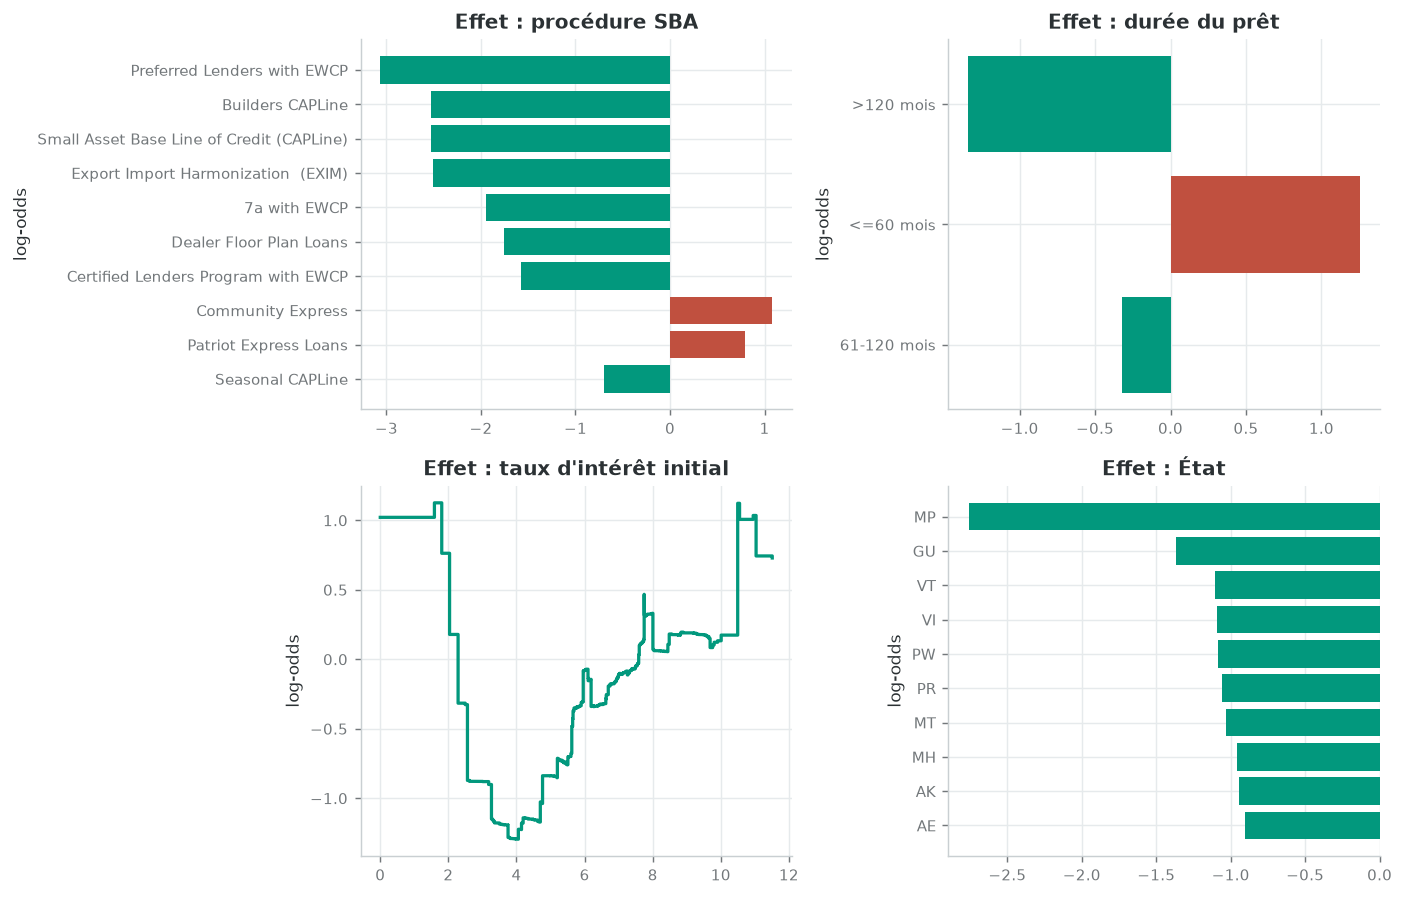
\includegraphics[width=\textwidth]{ebm_effets.png}
  \caption{Effet des quatre variables principales de l'EBM, en log-cote (rouge : augmente le risque ; vert : le
  réduit).}
  \label{fig:effets}
\end{figure}

\paragraph{Analyse des erreurs.} Au seuil qui maximise le F1, le modèle manque une majorité des défauts : le taux de
faux négatifs va de 57\,\% à 100\,\% selon l'État, et dépend fortement de la procédure (tableau~\ref{tab:erreurs}).
Pour les prêts des prêteurs certifiés, dont le taux de défaut est faible, presque aucun défaut n'est détecté. Le modèle
est donc un outil pour \emph{estimer et ordonner} un risque, pas pour détecter chaque défaut : c'est l'usage que nous en
faisons, puisque le MCDA utilise la probabilité et non une prédiction binaire.

\begin{table}[htbp]
\centering
\footnotesize\setlength{\tabcolsep}{4pt}
\caption{Analyse des erreurs de l'EBM par procédure (validation, seuil F1)}\label{tab:erreurs}
\begin{tabular}{lcccc}
\toprule
Procédure SBA & Prêts & Taux réel & PD moyenne & Faux négatifs \\
\midrule
SBA Express Program & 41\,517 & 4,0\,\% & 4,4\,\% & 61\,\% \\
Preferred Lenders Program & 20\,337 & 2,1\,\% & 2,0\,\% & 100\,\% \\
Small Loan Advantage Initiative & 9\,844 & 5,2\,\% & 3,6\,\% & 92\,\% \\
7a General & 5\,680 & 2,4\,\% & 2,5\,\% & 99\,\% \\
Patriot Express Loans & 1\,218 & 7,4\,\% & 6,7\,\% & 77\,\% \\
Working Capital CAPLine & 884 & 1,9\,\% & 2,0\,\% & 100\,\% \\
\bottomrule
\end{tabular}
\end{table}


% ---------------------------------------------------------------------------------------------
\section{Décision multicritère}

\subsection{Poids et filtre}

Les poids issus de l'AHP sont très proches des poids cibles (figure~\ref{fig:poids}), avec un ratio de cohérence de
0,009, bien inférieur au seuil de 0,10 ($\lambda_{\max} = 8{,}091$). Le filtre éliminatoire écarte 11 projets sur 40 :
8 pour un DSCR inférieur à 1 et 3 pour une probabilité de défaut supérieure à 7,1\,\%.

\begin{figure}[htbp]
  \centering
  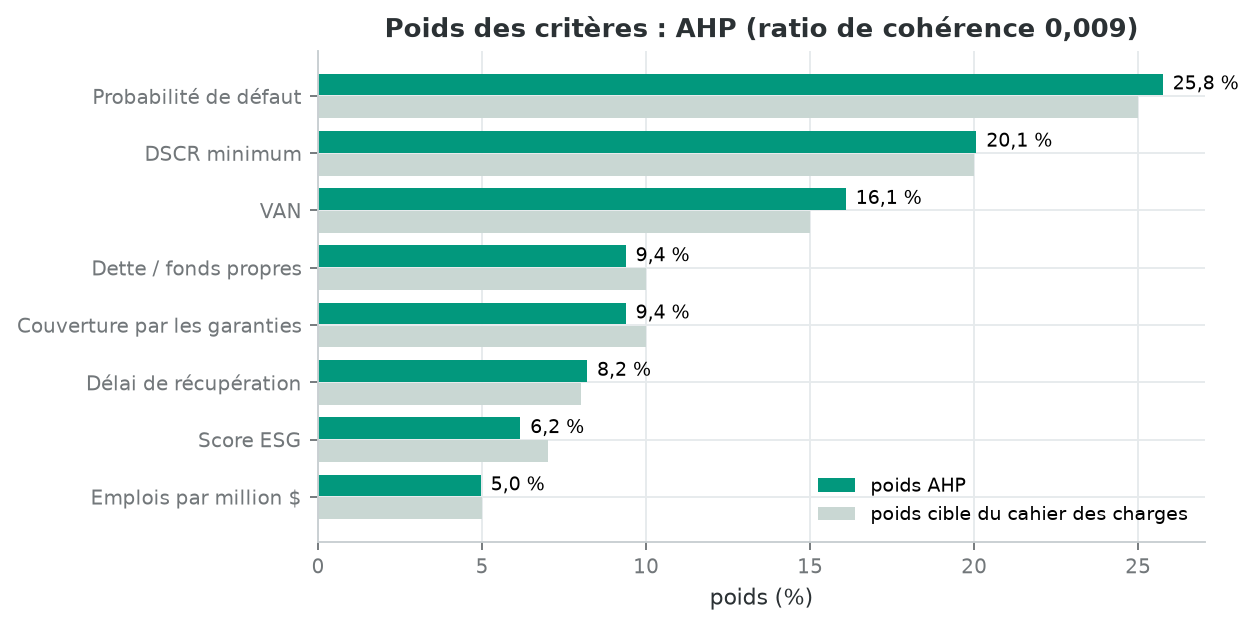
\includegraphics[width=0.8\textwidth]{mcda_poids.png}
  \caption{Poids des critères obtenus par AHP, comparés aux poids cibles.}
  \label{fig:poids}
\end{figure}

\subsection{Catégories et classement}

ELECTRE TRI (règle pessimiste, $\lambda = 0{,}6$) affecte \textbf{9 projets à \og Financer \fg{}, 19 à \og Financer
sous conditions \fg{} et 12 à \og Refuser \fg{}} (dont les 11 écartés par le filtre). La figure~\ref{fig:carte} situe
les 40 projets selon leur risque et leur DSCR : les projets à financer se concentrent dans la zone de faible risque et
de DSCR confortable, mais la catégorie dépend aussi des six autres critères, ce qui explique que des projets voisins
sur ce graphique soient classés différemment. Le classement ELECTRE III place en tête le Studio de développement
logiciel Murphy, l'Atelier d'insertion professionnelle Foster, le Bureau d'ingénierie Dubois, l'Entreprise de travaux
spécialisés Brooks et la Brasserie artisanale Garcia. La liste complète figure en annexe (tableau~\ref{tab:projets}).

\begin{figure}[htbp]
  \centering
  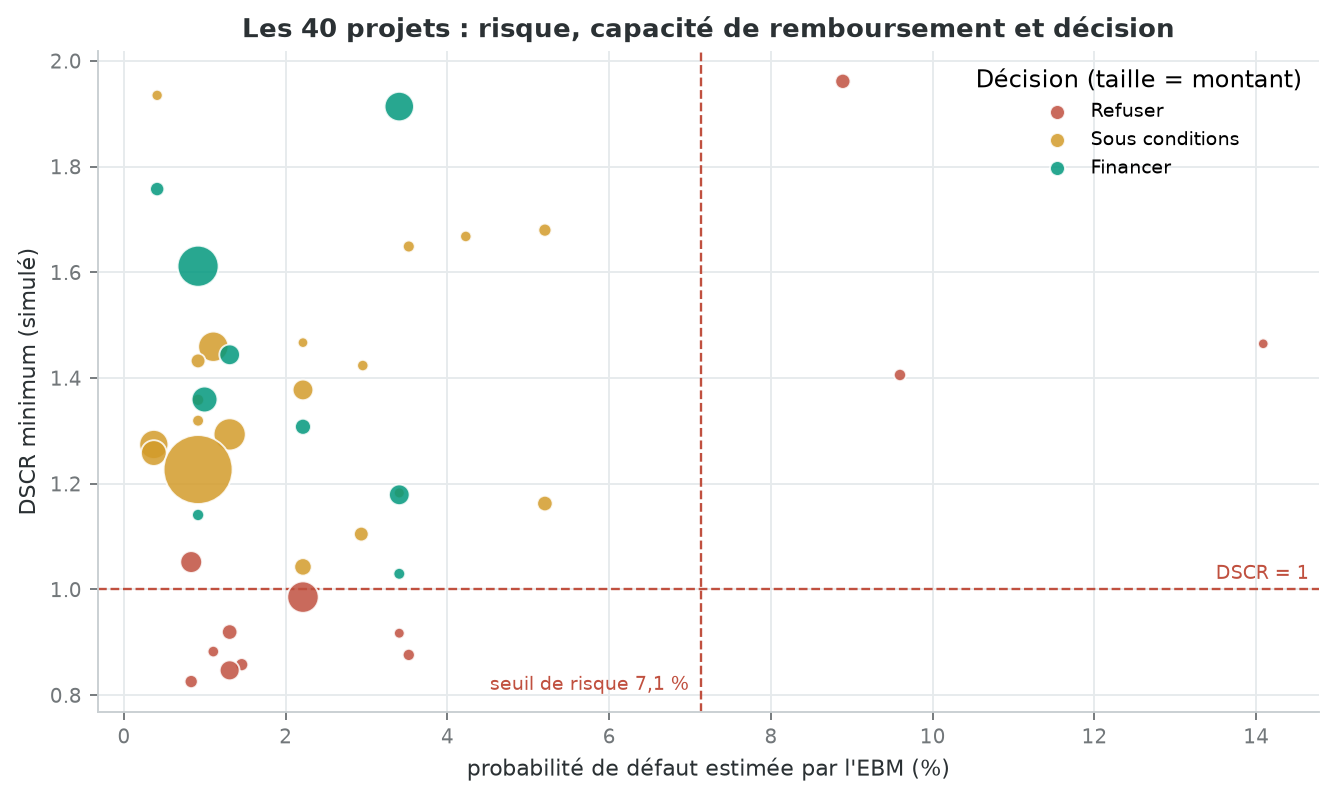
\includegraphics[width=0.9\textwidth]{mcda_carte.png}
  \caption{Les 40 projets selon leur probabilité de défaut et leur DSCR minimum ; couleur : décision ELECTRE TRI ;
  taille : montant demandé ; pointillés : seuils du filtre.}
  \label{fig:carte}
\end{figure}

Deux observations illustrent l'intérêt des méthodes de surclassement. Le Cabinet dentaire Baker a un risque très faible
(0,4\,\%) et un excellent score ESG, mais une VAN négative et un délai de récupération de 12,7 ans : il n'est que
\og sous conditions \fg{}, ses points forts ne compensant pas ses faiblesses. Par ailleurs, 7 projets ont une
\og position ambiguë \fg{} : les distillations descendante et ascendante les placent très différemment, ce qui signale
qu'ils sont incomparables à une partie des autres. Enfin, les règles pessimiste et optimiste d'ELECTRE TRI diffèrent
pour 15 projets : la règle pessimiste, retenue, est la plus prudente.

\subsection{Accord entre ELECTRE III et PROMETHEE II}

Les deux méthodes donnent des classements très proches pour les 29 projets non écartés (figure~\ref{fig:e3p2}) :
coefficient de Spearman de 0,891 et $\tau$ de Kendall de 0,724. Le classement ne dépend donc pas de façon critique de
la méthode choisie ; les écarts concernent surtout le milieu du classement, où les projets sont proches.

\begin{figure}[htbp]
  \centering
  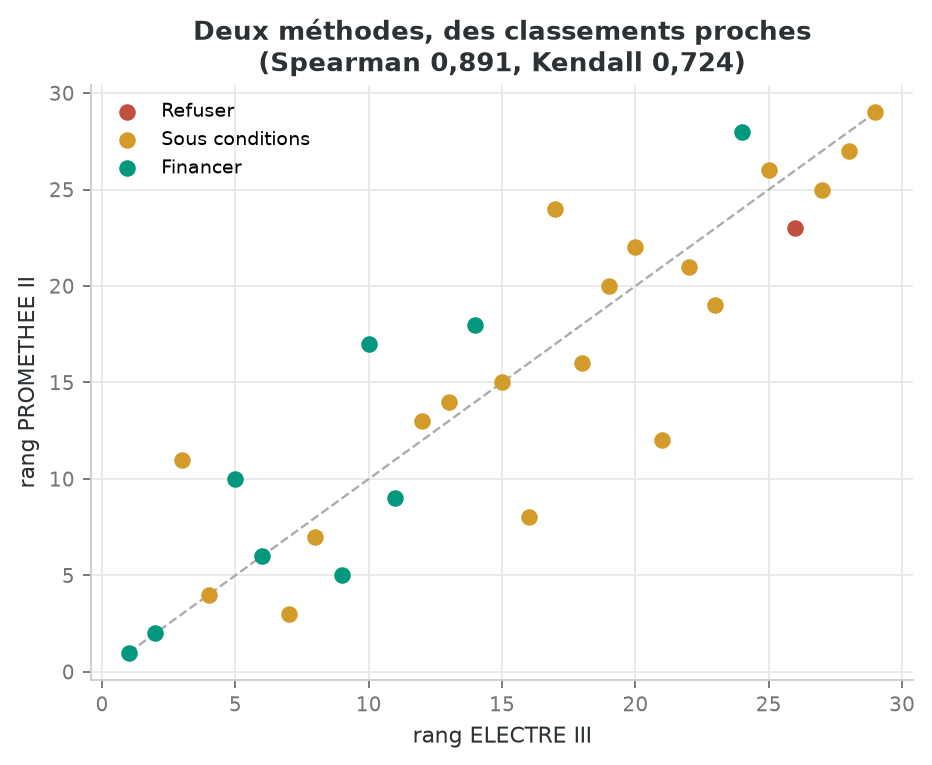
\includegraphics[width=0.55\textwidth]{mcda_e3_p2.png}
  \caption{Rangs ELECTRE III et PROMETHEE II des 29 projets non écartés.}
  \label{fig:e3p2}
\end{figure}

\subsection{Robustesse}

\paragraph{Un paramètre à la fois.} Le classement ELECTRE III bouge peu quand on modifie les seuils (Spearman de 0,937 à
0,976). Les catégories, elles, dépendent surtout de la coupure $\lambda$ (tableau~\ref{tab:sensibilite},
figure~\ref{fig:lambda}) : entre 0,5 et 0,8, 0 à 3 projets changent de catégorie, mais 10 changent à $\lambda = 0{,}9$
et 26 à $\lambda = 1$, valeur qui exige l'unanimité des critères. Un veto large ($v = 80\,\%$) modifie aussi 16
catégories.

\begin{table}[htbp]
\centering
\footnotesize\setlength{\tabcolsep}{4pt}
\caption{Sensibilité « un paramètre à la fois » (référence : q/p/v = 5/20/50\,\%, $\lambda$ = 0,6)}\label{tab:sensibilite}
\begin{tabular}{llccc}
\toprule
Paramètre & Valeur & Spearman & Kendall & Changements de catégorie \\
\midrule
Seuils q/p/v & 3\%/15\%/40\% & 0,937 & 0,793 & 4 \\
Seuils q/p/v & 5\%/20\%/50\% & 1,000 & 1,000 & 0 \\
Seuils q/p/v & 10\%/30\%/60\% & 0,976 & 0,882 & 8 \\
Seuils q/p/v & 5\%/20\%/80\% & 0,966 & 0,862 & 16 \\
Coupure $\lambda$ & 0,5 & 1,000 & 1,000 & 1 \\
Coupure $\lambda$ & 0,6 & 1,000 & 1,000 & 0 \\
Coupure $\lambda$ & 0,7 & 1,000 & 1,000 & 0 \\
Coupure $\lambda$ & 0,8 & 1,000 & 1,000 & 3 \\
Coupure $\lambda$ & 0,9 & 1,000 & 1,000 & 10 \\
Coupure $\lambda$ & 1 & 1,000 & 1,000 & 26 \\
\bottomrule
\end{tabular}
\end{table}


\begin{figure}[htbp]
  \centering
  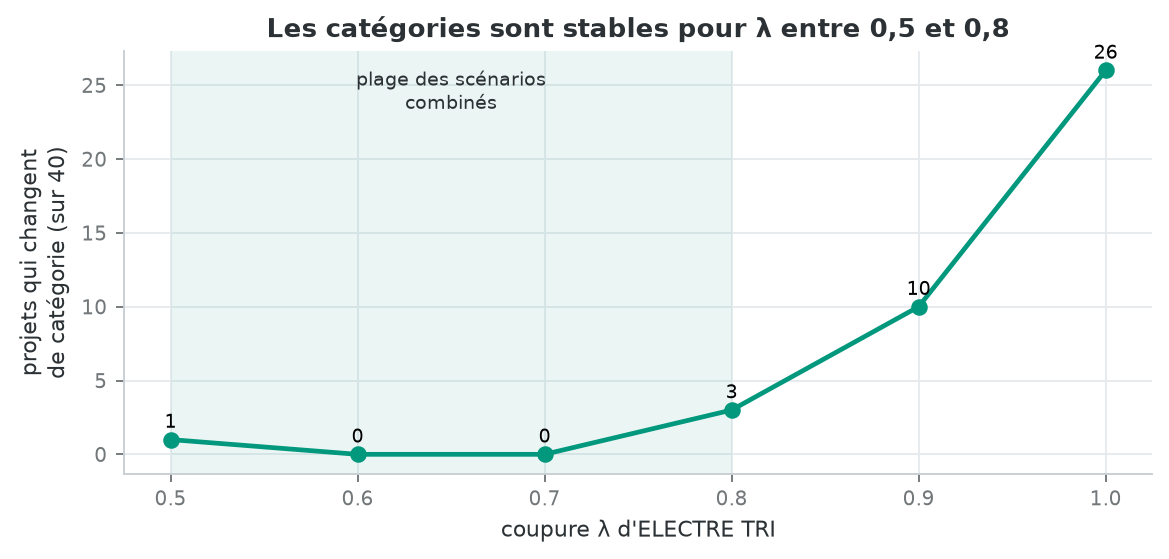
\includegraphics[width=0.75\textwidth]{mcda_lambda.png}
  \caption{Nombre de projets qui changent de catégorie selon la coupure $\lambda$.}
  \label{fig:lambda}
\end{figure}

\paragraph{Scénarios combinés et simulation.} Sur 200 scénarios faisant varier ensemble les poids, les seuils et
$\lambda$ (entre 0,5 et 0,8), 10 décisions sur 40 sont fragiles : 9 \og sous conditions \fg{} et 1 \og Refuser \fg{},
aucune parmi les \og Financer \fg{}. Les décisions de financement sont donc robustes aux paramètres de la méthode.
En revanche, avec les mêmes 40 prêts et 20 autres tirages des indicateurs simulés, un projet ne garde sa catégorie que
dans 48\,\% des cas en moyenne (figure~\ref{fig:stabilite}) : les catégories dépendent autant de la simulation que des
projets. C'est la principale limite de la démonstration, et la raison d'être de l'outil réutilisable, qui permet
d'appliquer la même méthode à des indicateurs réels.

\begin{figure}[htbp]
  \centering
  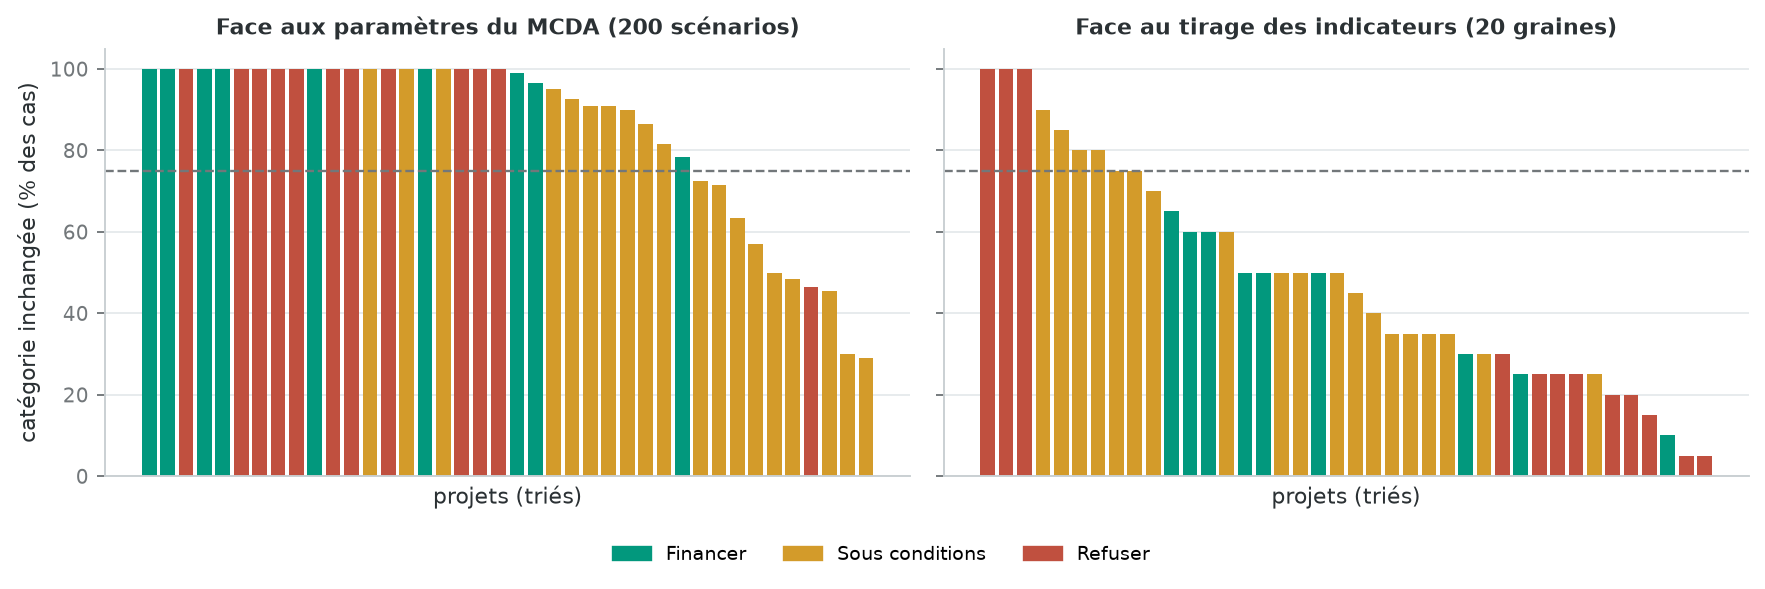
\includegraphics[width=\textwidth]{mcda_stabilite.png}
  \caption{Part des cas où la catégorie de chaque projet est inchangée : face aux paramètres du MCDA (gauche) et face
  au tirage des indicateurs simulés (droite).}
  \label{fig:stabilite}
\end{figure}

% ---------------------------------------------------------------------------------------------
\section{Arbitrage sous budget}

Avec un budget de 5\,M\$, la règle \og suivre le classement \fg{} retient \textbf{11 projets} (8 \og Financer \fg{} et
3 \og sous conditions \fg{}) pour 4,98\,M\$ engagés, soit 99,6\,\% du budget, répartis sur 7 secteurs
(figure~\ref{fig:arbitrage}). Un seul projet \og Financer \fg{} n'est pas retenu, les Pompes funèbres Price, parce que
son secteur atteint déjà le plafond de 35\,\% avec le Studio Murphy. Trois projets sont hors des bornes de montant,
dont le Garde-meubles Grant (5\,M\$, soit la totalité du budget).

\begin{figure}[htbp]
  \centering
  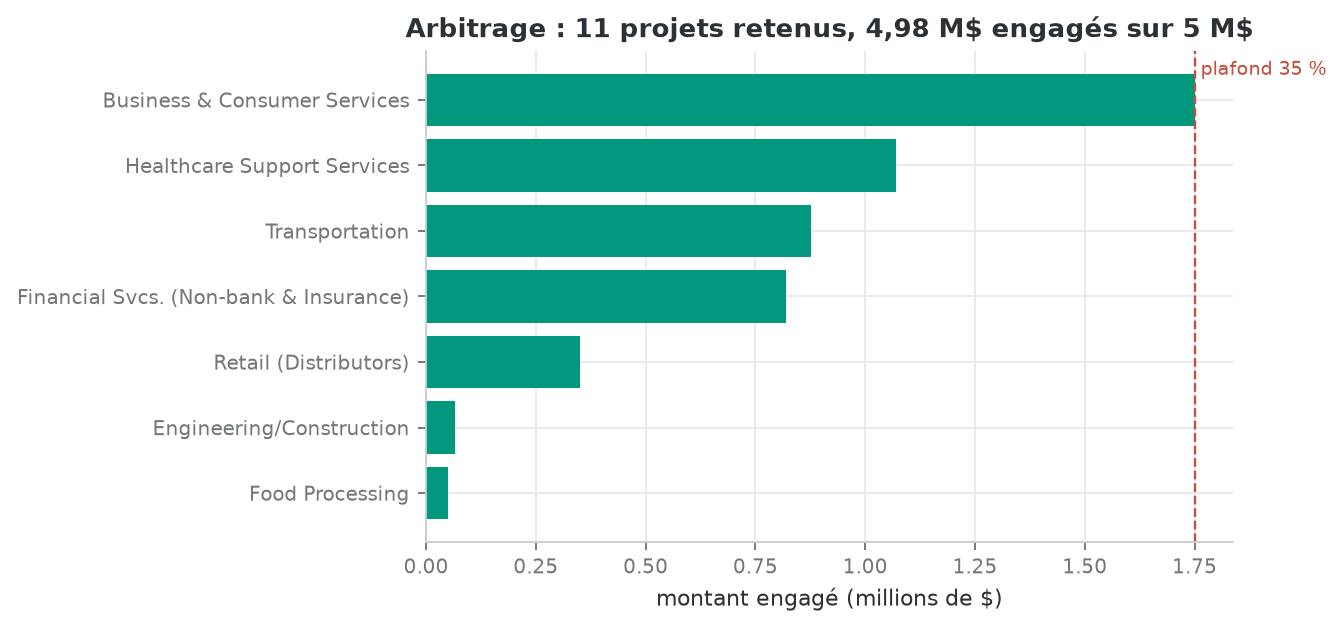
\includegraphics[width=0.85\textwidth]{arbitrage_secteurs.png}
  \caption{Montant engagé par secteur (règle \og suivre le classement \fg{}) ; pointillés : plafond sectoriel.}
  \label{fig:arbitrage}
\end{figure}

Le tableau~\ref{tab:arbitrage-regles} compare les deux règles. Maximiser le nombre de projets en finance 21 dans 11
secteurs, mais écarte le projet classé premier, le Studio Murphy (1,7\,M\$), au profit de plusieurs petits projets.
Ce résultat montre que l'objectif de l'optimisation n'est pas un détail technique : il traduit une politique. Nous
retenons par défaut la règle qui respecte le classement du comité, et proposons l'autre comme éclairage.

\begin{table}[htbp]
\centering
\small\setlength{\tabcolsep}{4pt}
\caption{Comparaison des deux règles de sélection (budget 5\,M\$, 20\,000 à 2\,M\$ par projet, 35\,\% au plus par secteur)}\label{tab:arbitrage-regles}
\begin{tabular}{lccccccc}
\toprule
Règle & Retenus & Financer & Sous cond. & Engagé & Utilisation & Secteurs & N\textsuperscript{o}\,1 financé \\
\midrule
Suivre le classement & 11 & 8 & 3 & 4,98\,M\$ & 99,6\,\% & 7 & oui \\
Maximiser le nombre & 21 & 8 & 13 & 4,89\,M\$ & 97,8\,\% & 11 & \textbf{non} \\
\bottomrule
\end{tabular}
\end{table}


% ---------------------------------------------------------------------------------------------
\section{Contrôle a posteriori}

Parmi les 40 prêts de démonstration, 3 ont réellement fait défaut dans les 60 mois. Les trois sont classés
\og Refuser \fg{} ; aucun des 9 projets \og Financer \fg{} ni des 19 \og sous conditions \fg{} n'a fait défaut.
La vraie issue n'est lue qu'après les décisions et n'entre dans aucun calcul. Avec trois cas, ce résultat est une
illustration encourageante, pas une preuve.

% =============================================================================================
\chapter{Solution déployée}\label{chap:solution}

La solution est une application web Streamlit, déployée sur Streamlit Community Cloud à partir du dépôt GitHub, aux
couleurs de l'École Centrale Casablanca. Elle ne se limite pas à présenter nos 40 projets : n'importe quel jeu de
projets peut y être importé et évalué avec ses propres critères, poids, filtres et budget.

% ---------------------------------------------------------------------------------------------
\section{Fonctionnement}

L'application ne fait qu'\emph{afficher} des résultats et déclencher des calculs déterministes. Les résultats du
pipeline (projets, modèle entraîné, métriques, figures, paramètres) sont calculés à l'avance et versionnés dans le
dépôt, ce qui permet de démarrer sans base de données ni données brutes. Au premier passage, l'application évalue la
démonstration (environ 4 secondes, robustesse comprise) et met le résultat en cache. L'analyse active vit dans la
mémoire de session de chaque visiteur : si un utilisateur importe son propre jeu, les autres continuent de voir la
démonstration. La clé du modèle de langage est stockée dans les secrets de la plateforme et n'apparaît jamais dans le
code ni dans les messages.

\begin{figure}[htbp]
\centering
\begin{tikzpicture}[font=\small,
  box/.style={draw=eccgris,rounded corners=3pt,align=center,minimum height=0.95cm,fill=white},
  arr/.style={-{Stealth[length=2mm]},eccgris,thick}]
  \node[box,text width=4.2cm] (user) at (0,0) {\textbf{Utilisateur}\\ navigateur web};
  \node[box,text width=4.2cm] (gh) at (8,0) {\textbf{Dépôt GitHub}\\ code et résultats};
  \node[box,text width=9.2cm] (app) at (2.5,-1.9) {\textbf{app.py et pages} : affichage, 8 pages, barre latérale};
  \node[box,text width=9.2cm,draw=eccvert,line width=1pt,fill=eccclair] (state) at (2.5,-3.3)
       {\textbf{Analyse active} : jeu de projets, configuration, résultats (session et cache)};
  \node[box,text width=4.4cm] (eng) at (0.1,-4.9) {\textbf{Moteur}\\ filtre, MCDA, arbitrage};
  \node[box,text width=4.4cm] (ia) at (4.9,-4.9) {\textbf{IA}\\ agent rédacteur, conseiller};
  \node[box,text width=9.2cm] (files) at (2.5,-6.4) {\textbf{Fichiers du pipeline} : projets, modèle, métriques, figures};
  \node[box,text width=2.6cm] (gem) at (9.0,-4.9) {\textbf{Gemini}\\ API, clé secrète};
  \begin{scope}[on background layer]
    \node[draw=eccgris,dashed,rounded corners=5pt,fit=(app)(state)(eng)(ia)(files),inner sep=8pt,
          label={[text=eccgris,font=\scriptsize]north east:Streamlit Community Cloud}] {};
  \end{scope}
  \draw[arr,{Stealth[length=2mm]}-{Stealth[length=2mm]}] (user) -- (user|-app.north);
  \draw[arr] (gh) -- node[right,font=\scriptsize,text=eccgris]{à chaque mise à jour} (gh|-app.north);
  \draw[arr] (app) -- (state);
  \draw[arr] (state.south-|eng.north) -- (eng);
  \draw[arr] (state.south-|ia.north) -- (ia);
  \draw[arr] (files.north-|eng.south) -- (eng);
  \draw[arr] (ia) -- (gem);
\end{tikzpicture}
\caption{Architecture de l'application : les pages affichent, le moteur calcule, le modèle de langage ne fait que
rédiger.}
\label{fig:archi-app}
\end{figure}

% ---------------------------------------------------------------------------------------------
\section{Les pages de l'application}

\paragraph{Tableau de bord.} Six cartes de chiffres clés, une carte des projets selon deux critères au choix avec les
seuils du filtre, le classement ELECTRE III et un tableau filtrable et téléchargeable de tous les projets, avec leurs
critères, leurs rangs et les indicateurs de fragilité (figure~\ref{fig:app-dashboard}).

\begin{figure}[htbp]
  \centering
  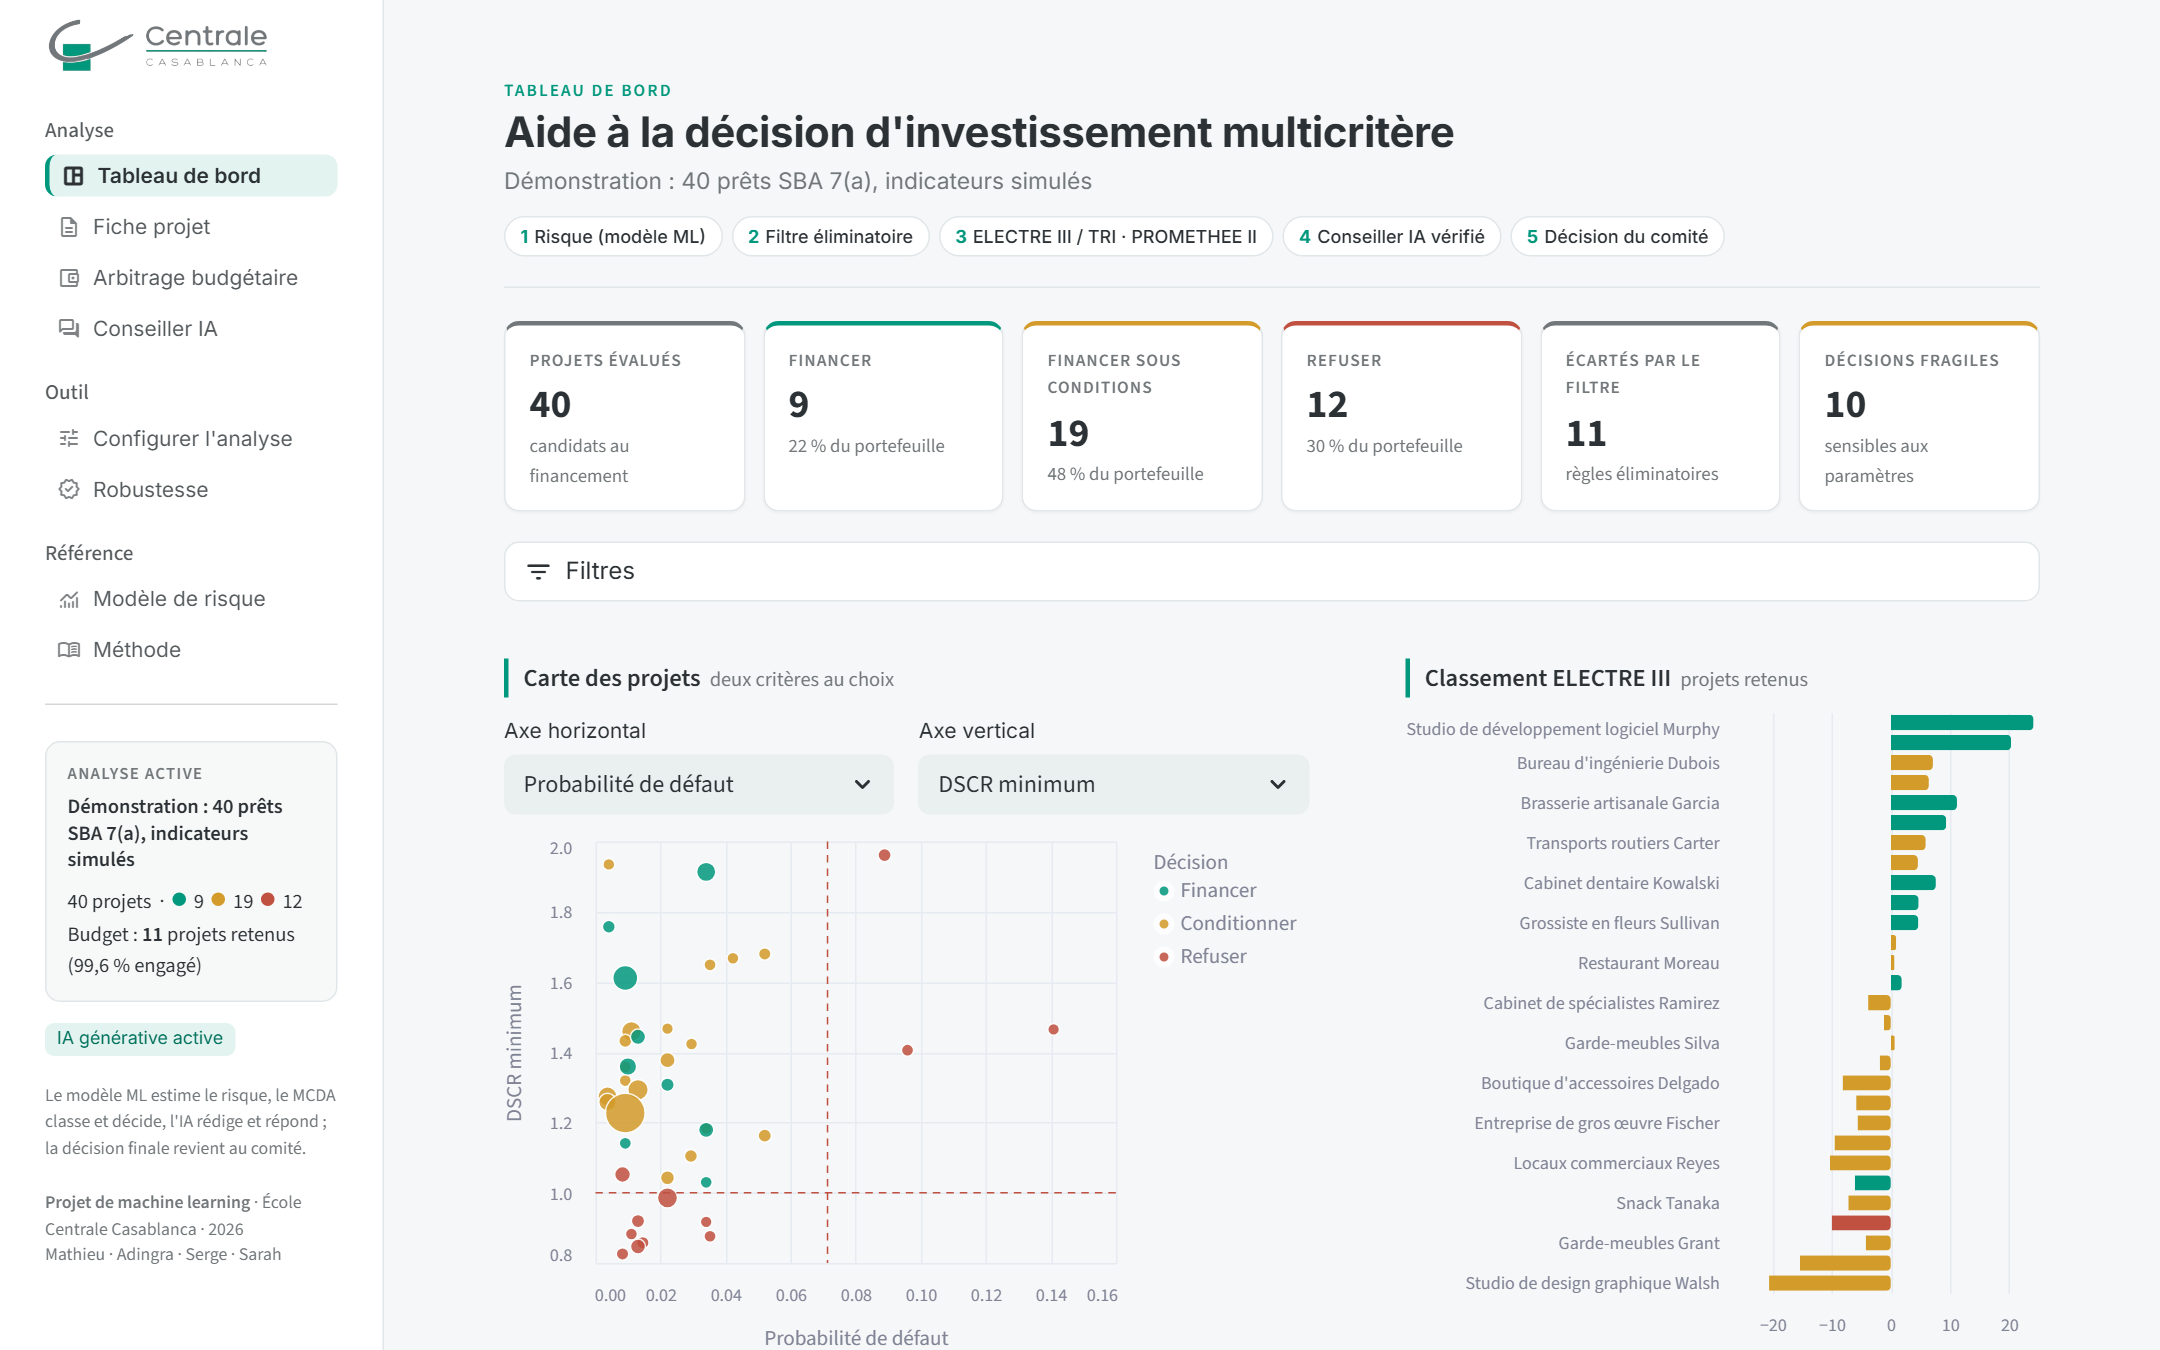
\includegraphics[width=\textwidth]{app_tableau_de_bord.png}
  \caption{Tableau de bord de l'application.}
  \label{fig:app-dashboard}
\end{figure}

\paragraph{Fiche projet.} Pour un projet choisi : sa catégorie, ses rangs, son statut budgétaire, puis un graphique
qui situe chaque critère par rapport aux profils d'ELECTRE TRI (zones Refuser, Conditionner, Financer), les facteurs
de risque issus de l'EBM, la fragilité et la note de l'agent rédacteur (figure~\ref{fig:app-fiche}). On y voit d'un
coup d'œil pourquoi le Cabinet dentaire Baker n'est que \og sous conditions \fg{} : risque, ESG et levier dans la zone
verte, VAN, délai et emplois dans la zone rouge.

\begin{figure}[htbp]
  \centering
  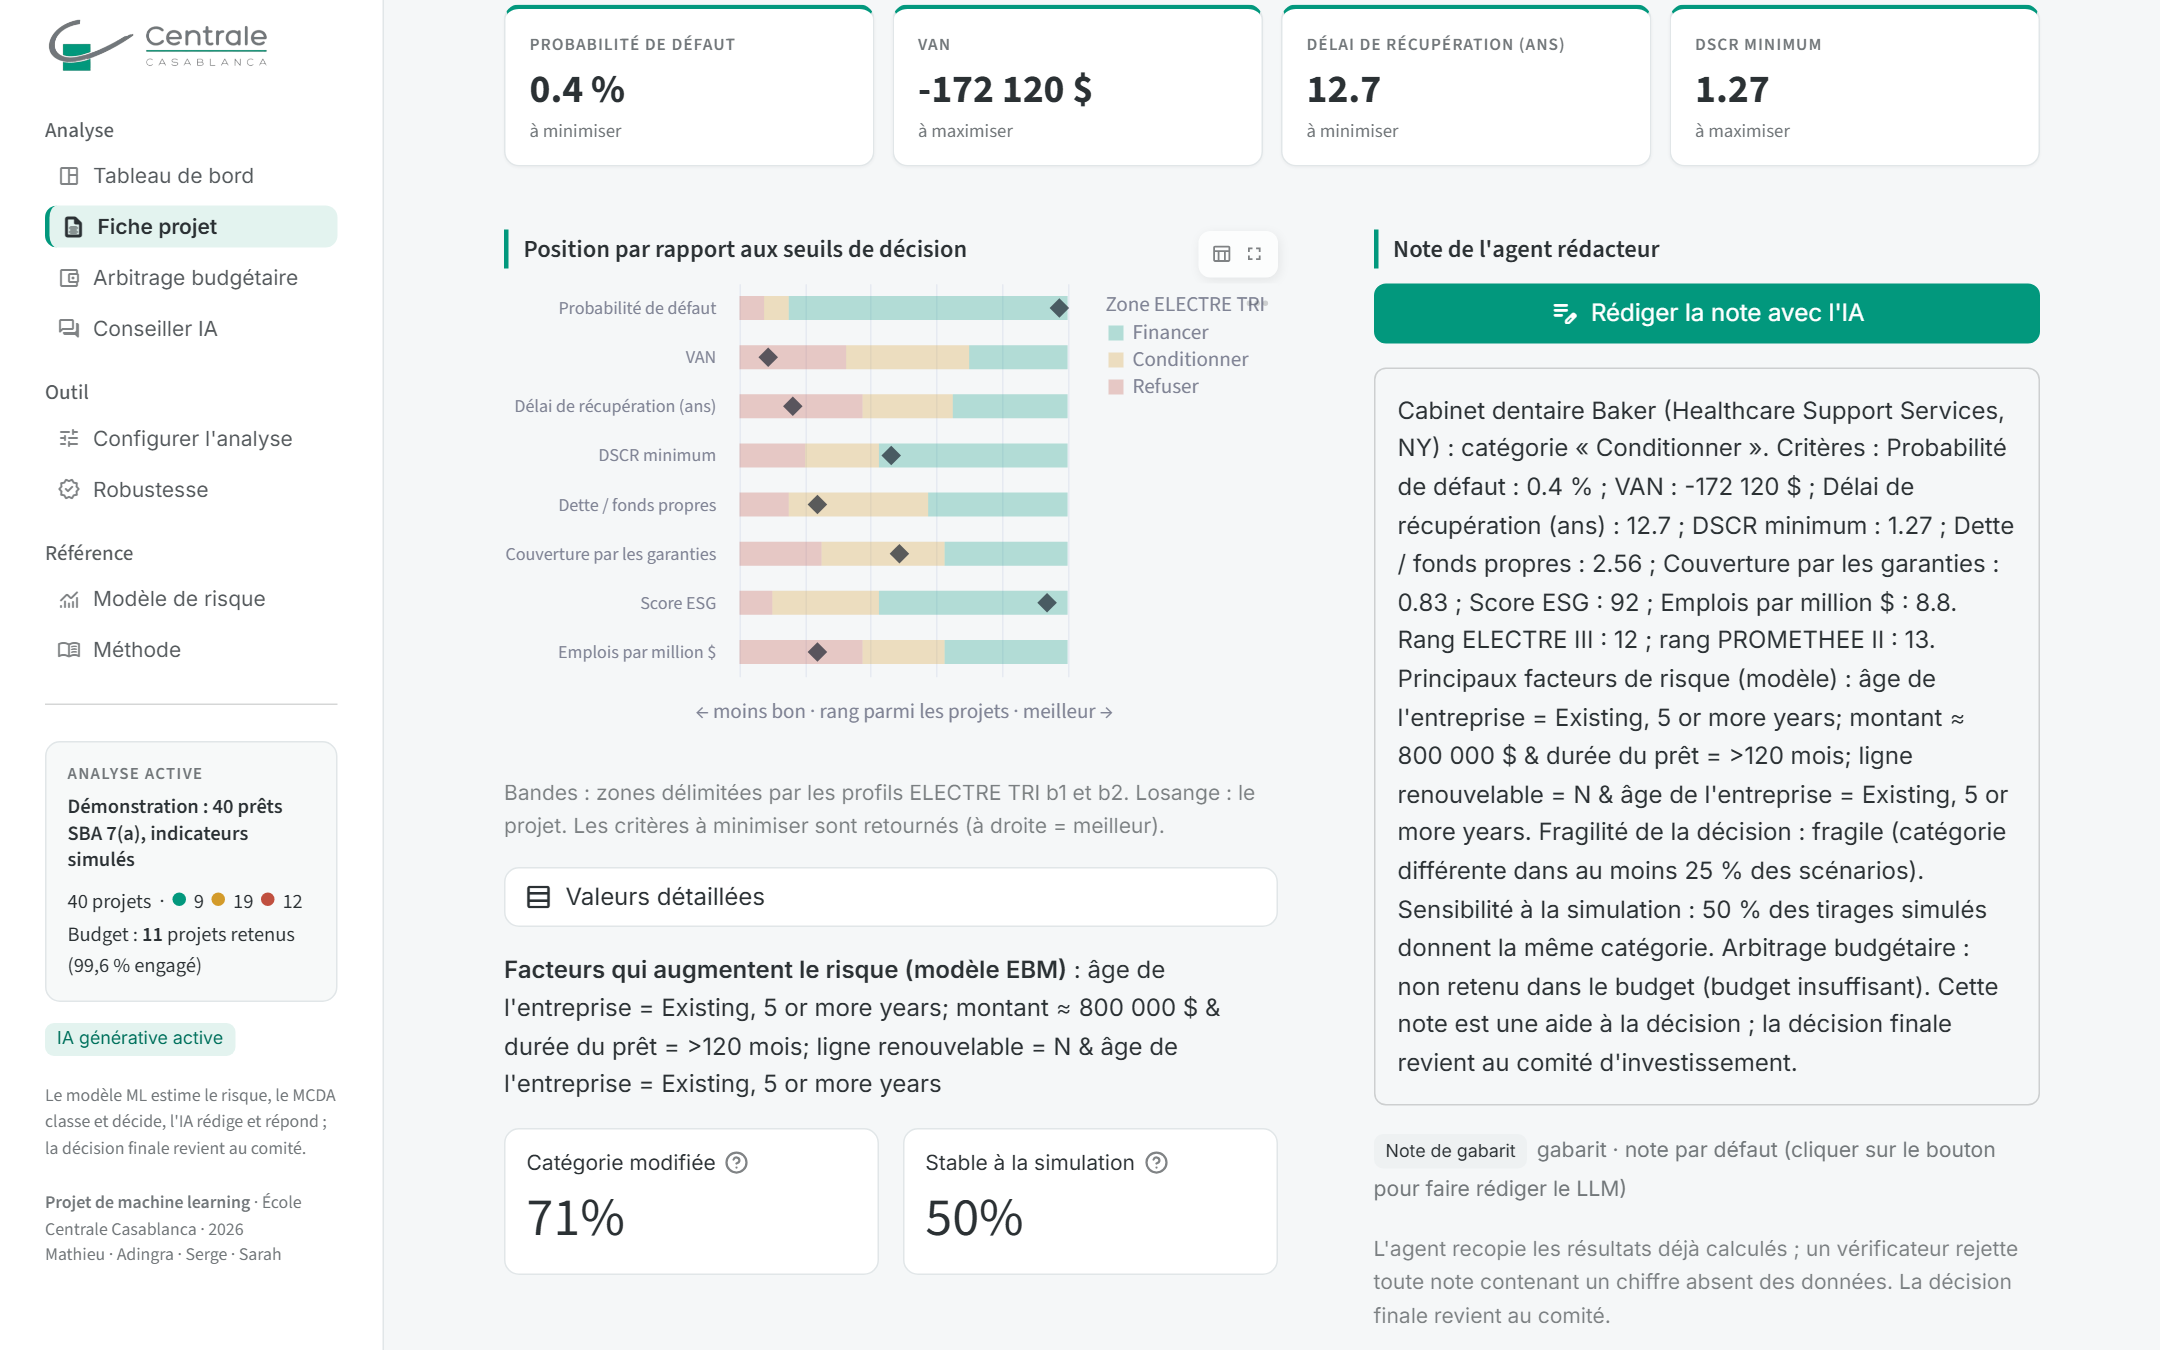
\includegraphics[width=\textwidth]{app_fiche_projet.png}
  \caption{Fiche projet du Cabinet dentaire Baker : position par rapport aux seuils et note de l'agent.}
  \label{fig:app-fiche}
\end{figure}

\paragraph{Arbitrage budgétaire.} Les paramètres du comité (budget, bornes, plafond sectoriel, inclusion des projets
sous conditions, règle de sélection) se règlent en direct ; la page montre le montant engagé, les secteurs financés,
les motifs de non-sélection et la décision projet par projet (figure~\ref{fig:app-arbitrage}).

\begin{figure}[htbp]
  \centering
  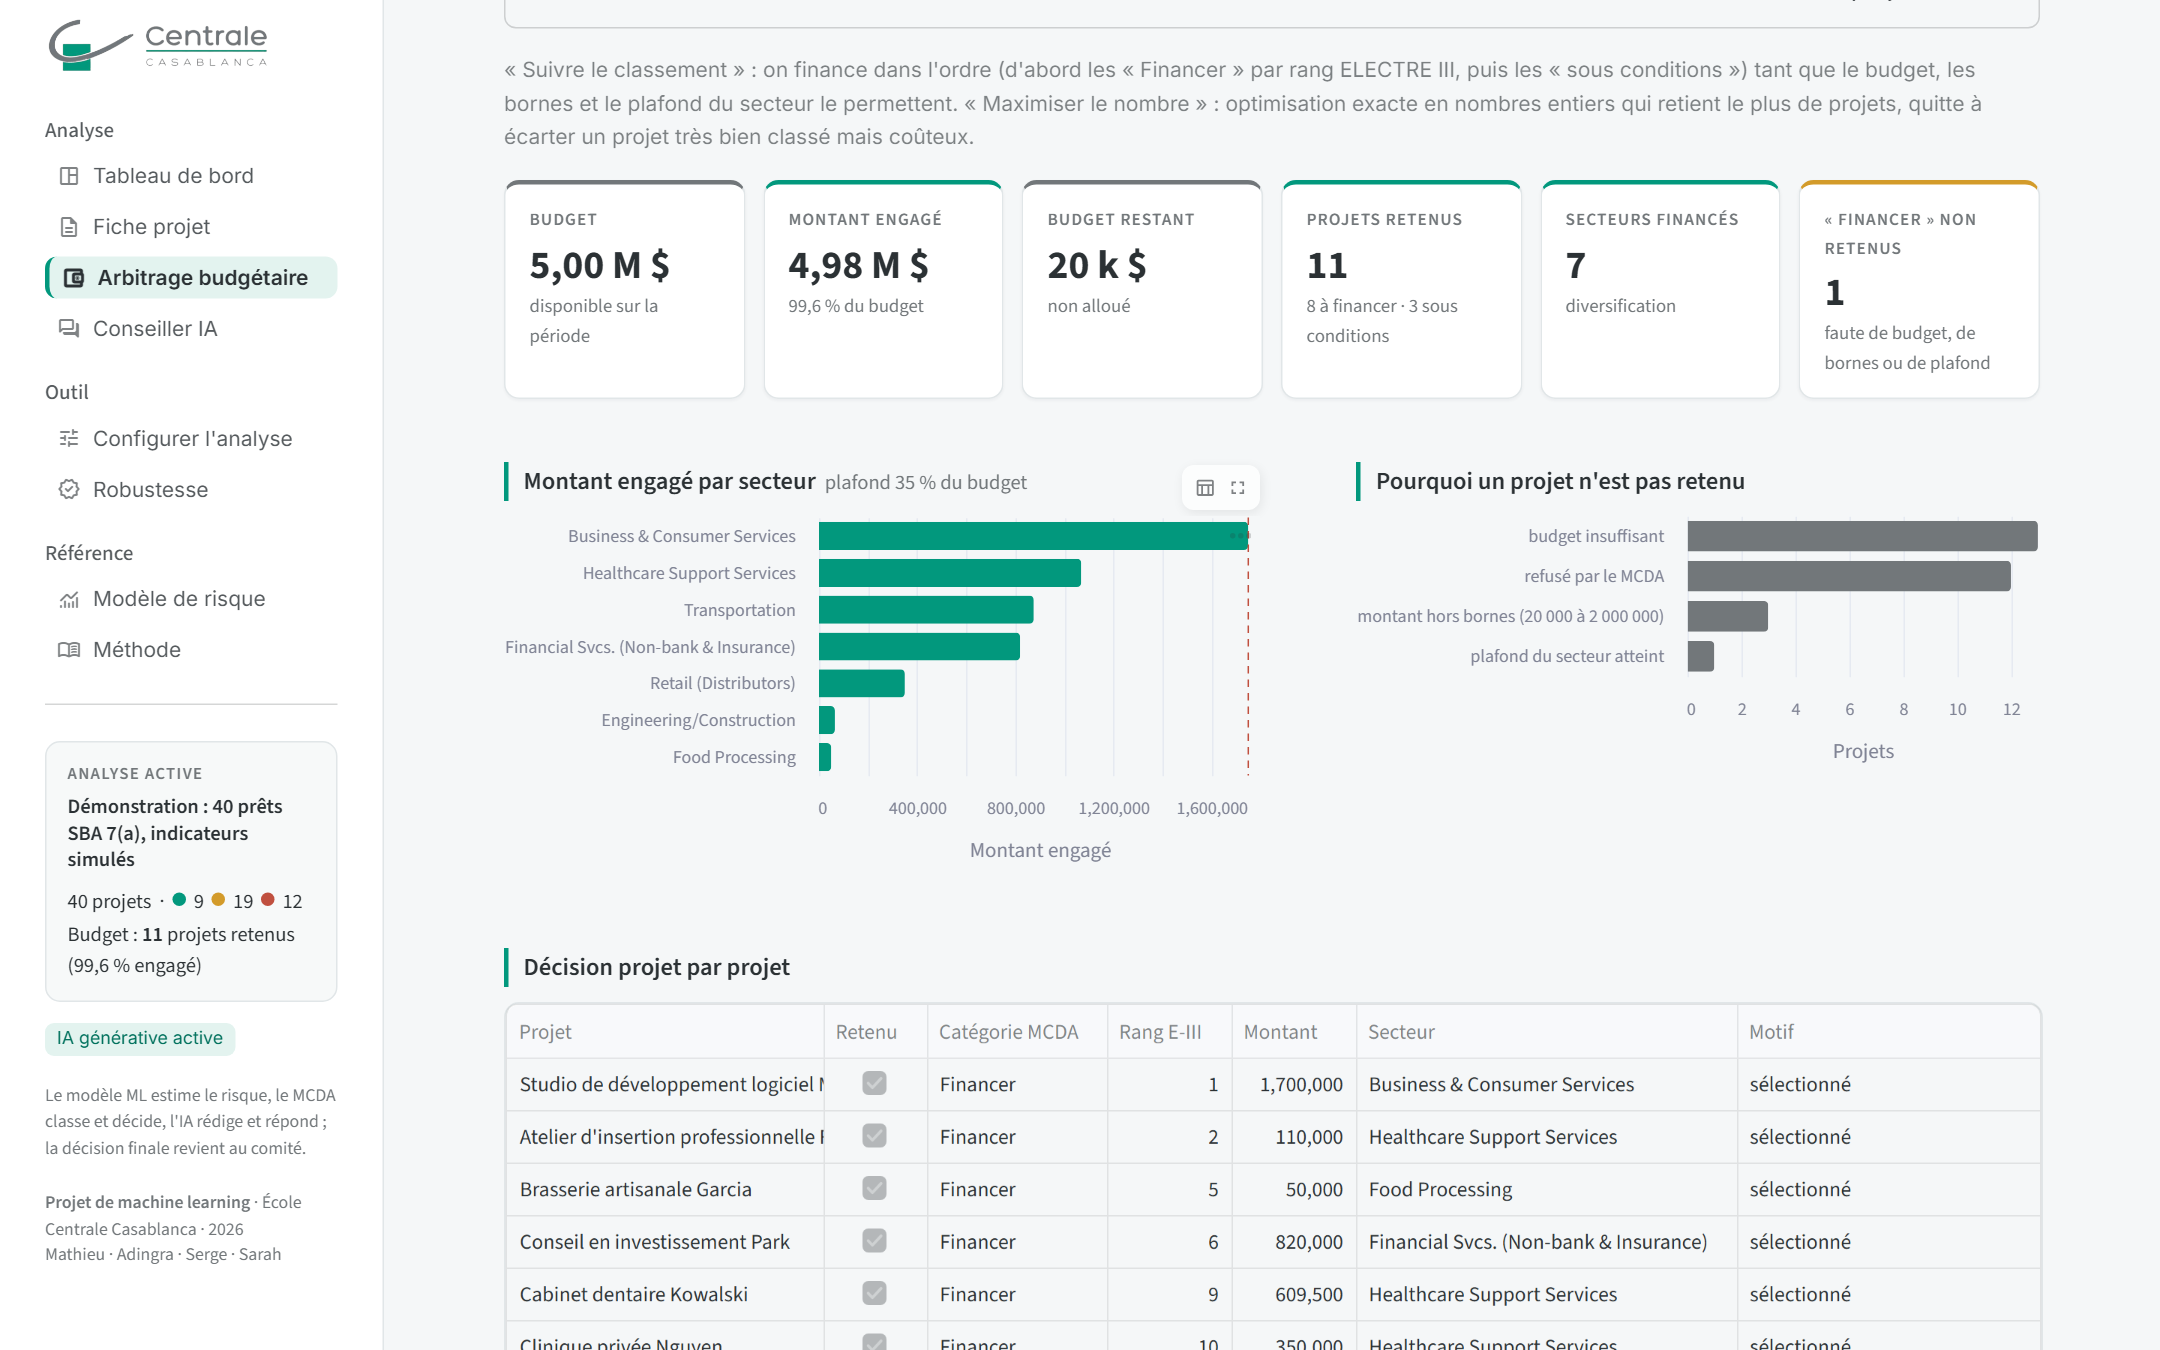
\includegraphics[width=\textwidth]{app_arbitrage.png}
  \caption{Arbitrage budgétaire : chiffres clés, montant par secteur et motifs de non-sélection.}
  \label{fig:app-arbitrage}
\end{figure}

\paragraph{Conseiller IA.} On pose une question en français ; le conseiller appelle ses outils et rédige une réponse
dont les nombres sont vérifiés. La figure~\ref{fig:app-conseiller} montre la réponse à la question \og Donne-moi les
détails du projet Garde-meubles Silva si l'ESG pèse 20\,\% et la VAN 30\,\% \fg{} : le conseiller a relancé le MCDA
avec ces poids, constaté que le projet passe de \og sous conditions \fg{} à \og Financer \fg{} (rang 17 à 15), et
signale que tous ses chiffres viennent des données consultées.

\begin{figure}[htbp]
  \centering
  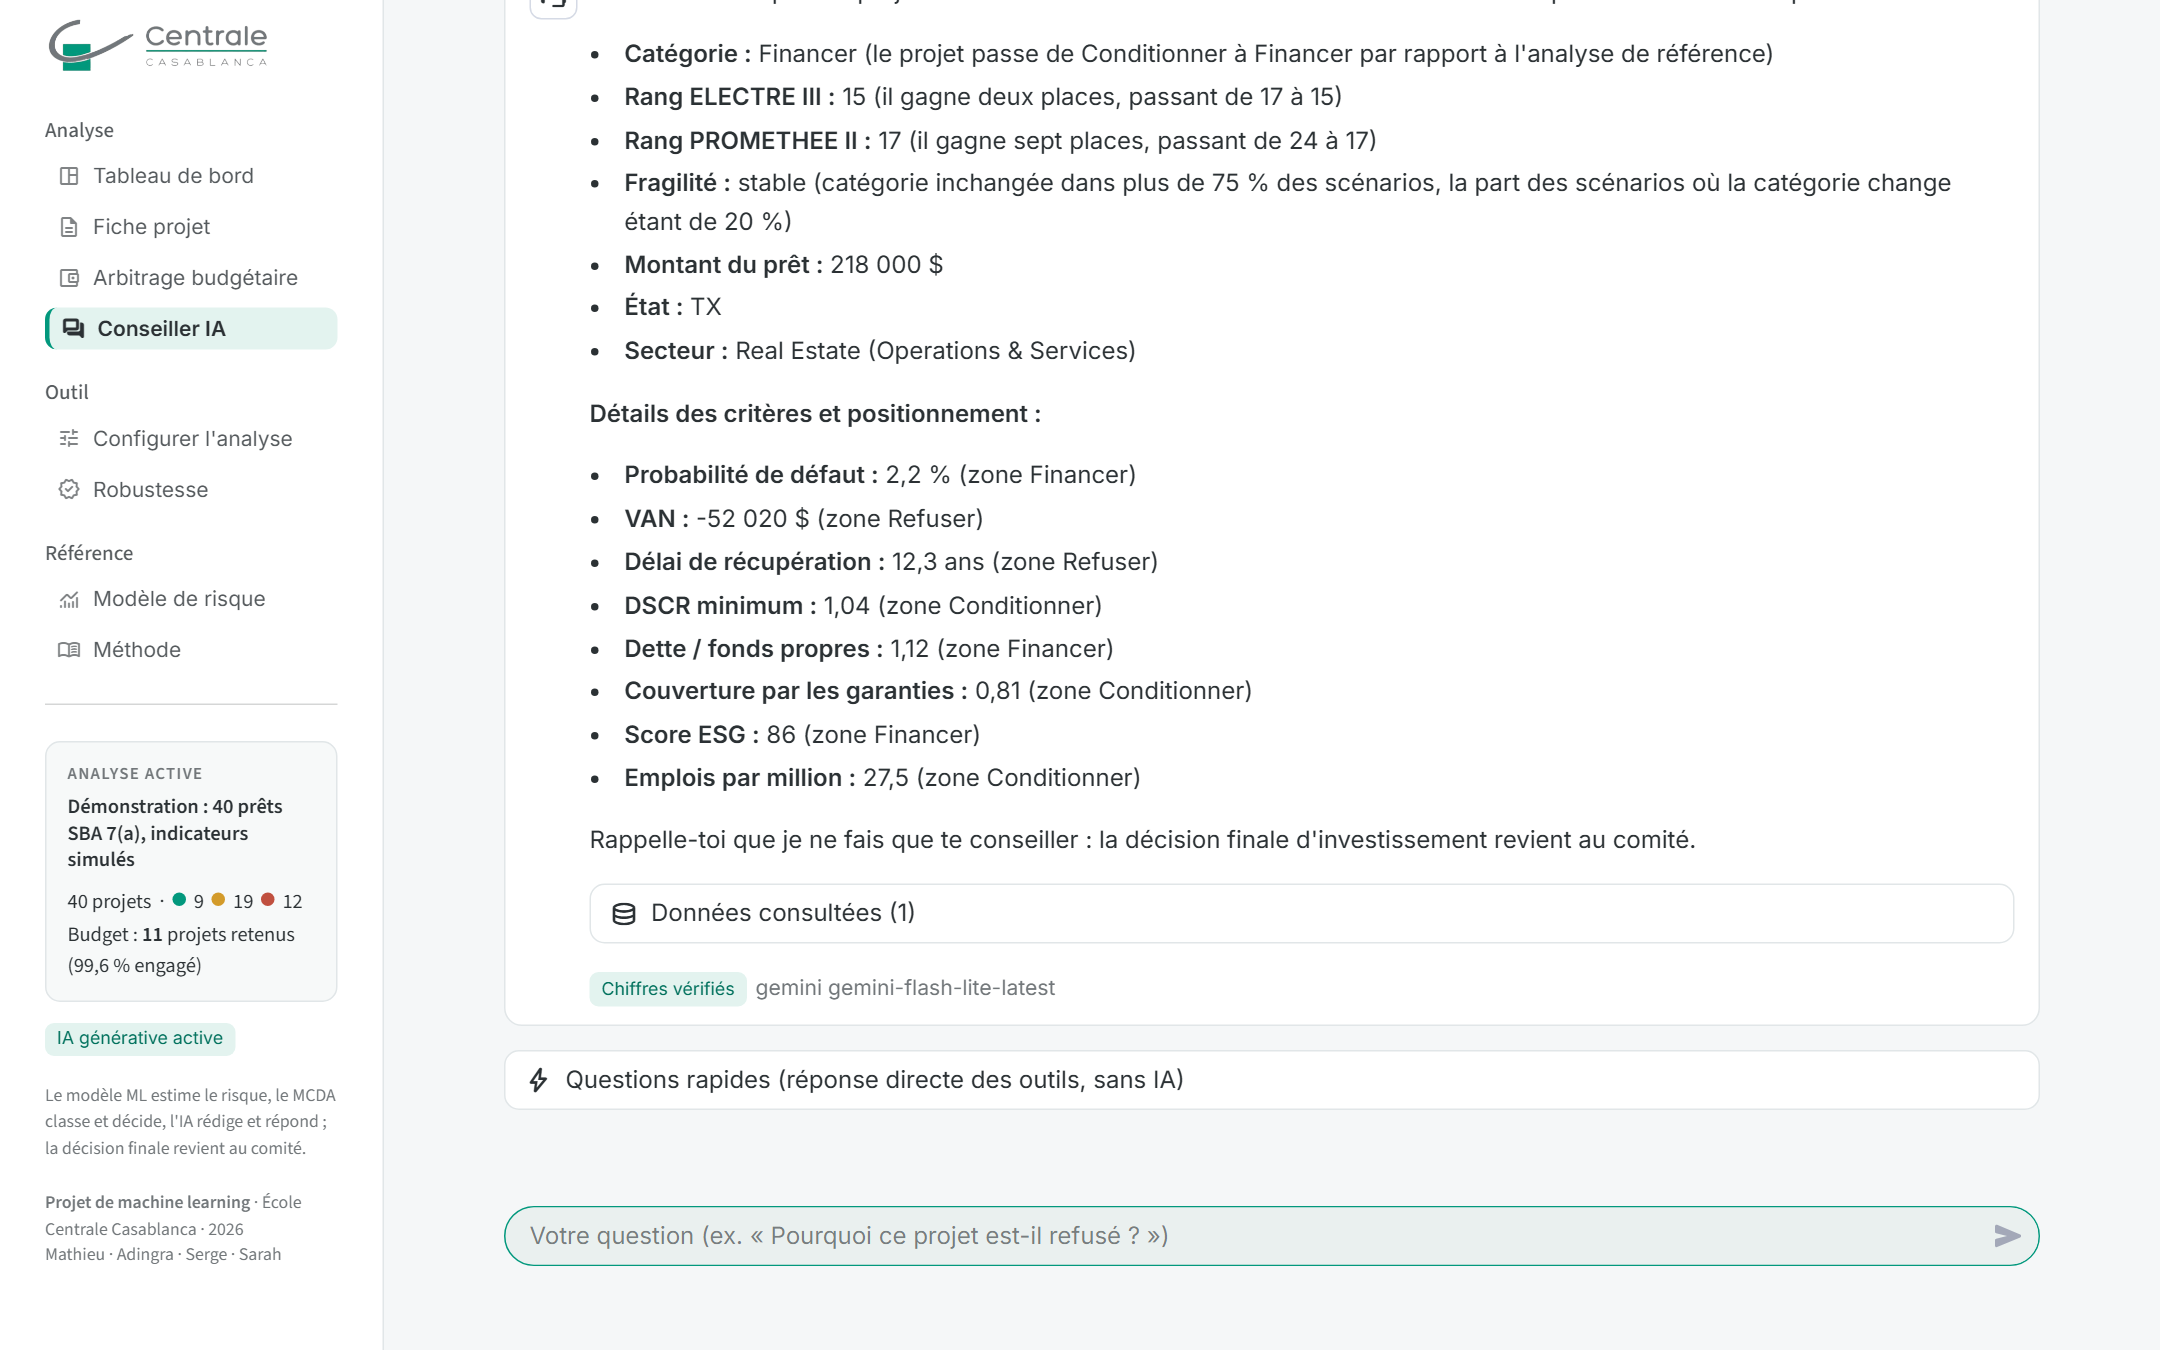
\includegraphics[width=\textwidth]{app_conseiller.png}
  \caption{Réponse du conseiller IA à une question de scénario, avec l'étiquette \og Chiffres vérifiés \fg{}.}
  \label{fig:app-conseiller}
\end{figure}

\paragraph{Configurer l'analyse, Robustesse, Modèle de risque, Méthode.} Les quatre autres pages permettent de
configurer une nouvelle analyse (section suivante), d'examiner la sensibilité des décisions, de consulter les
performances et les explications du modèle de risque, et de lire la méthode avec ses paramètres actifs et ses limites.

% ---------------------------------------------------------------------------------------------
\section{Un outil réutilisable}

La page \og Configurer l'analyse \fg{} transforme la démonstration en outil (figure~\ref{fig:app-config}) :

\begin{enumerate}
  \item \textbf{données} : import d'un fichier CSV ou Excel, une ligne par projet ; les nombres écrits à la française
        sont reconnus ; si le fichier décrit des prêts au format SBA sans probabilité de défaut, le modèle de risque la
        calcule ;
  \item \textbf{critères} : choix des colonnes, du libellé, du sens (deviné d'après le nom : un coût, un risque ou un
        délai est à minimiser), du poids et des profils $b_1$ et $b_2$ ;
  \item \textbf{pondération} : poids saisis ou AHP, avec la matrice des comparaisons et le ratio de cohérence
        affiché en direct ;
  \item \textbf{filtre} : autant de règles \og colonne, opérateur, seuil \fg{} que voulu ;
  \item \textbf{ELECTRE} : seuils $q$, $p$, $v$ et coupure $\lambda$.
\end{enumerate}
Tant qu'une erreur subsiste (valeur manquante, poids nuls, AHP incohérent), un message l'explique et le calcul est
bloqué. La configuration s'enregistre et se recharge en JSON, et la même évaluation est disponible en ligne de
commande. Quatre jeux de test fictifs accompagnent l'outil : 15 PME du Grand Casablanca en dirhams avec une
configuration AHP, 10 prêts au format SBA, 8 projets d'énergie avec des critères entièrement différents (taux de
rendement interne, coût par mégawatt, CO$_2$ évité, risque pays) et un fichier volontairement erroné.

\begin{figure}[htbp]
  \centering
  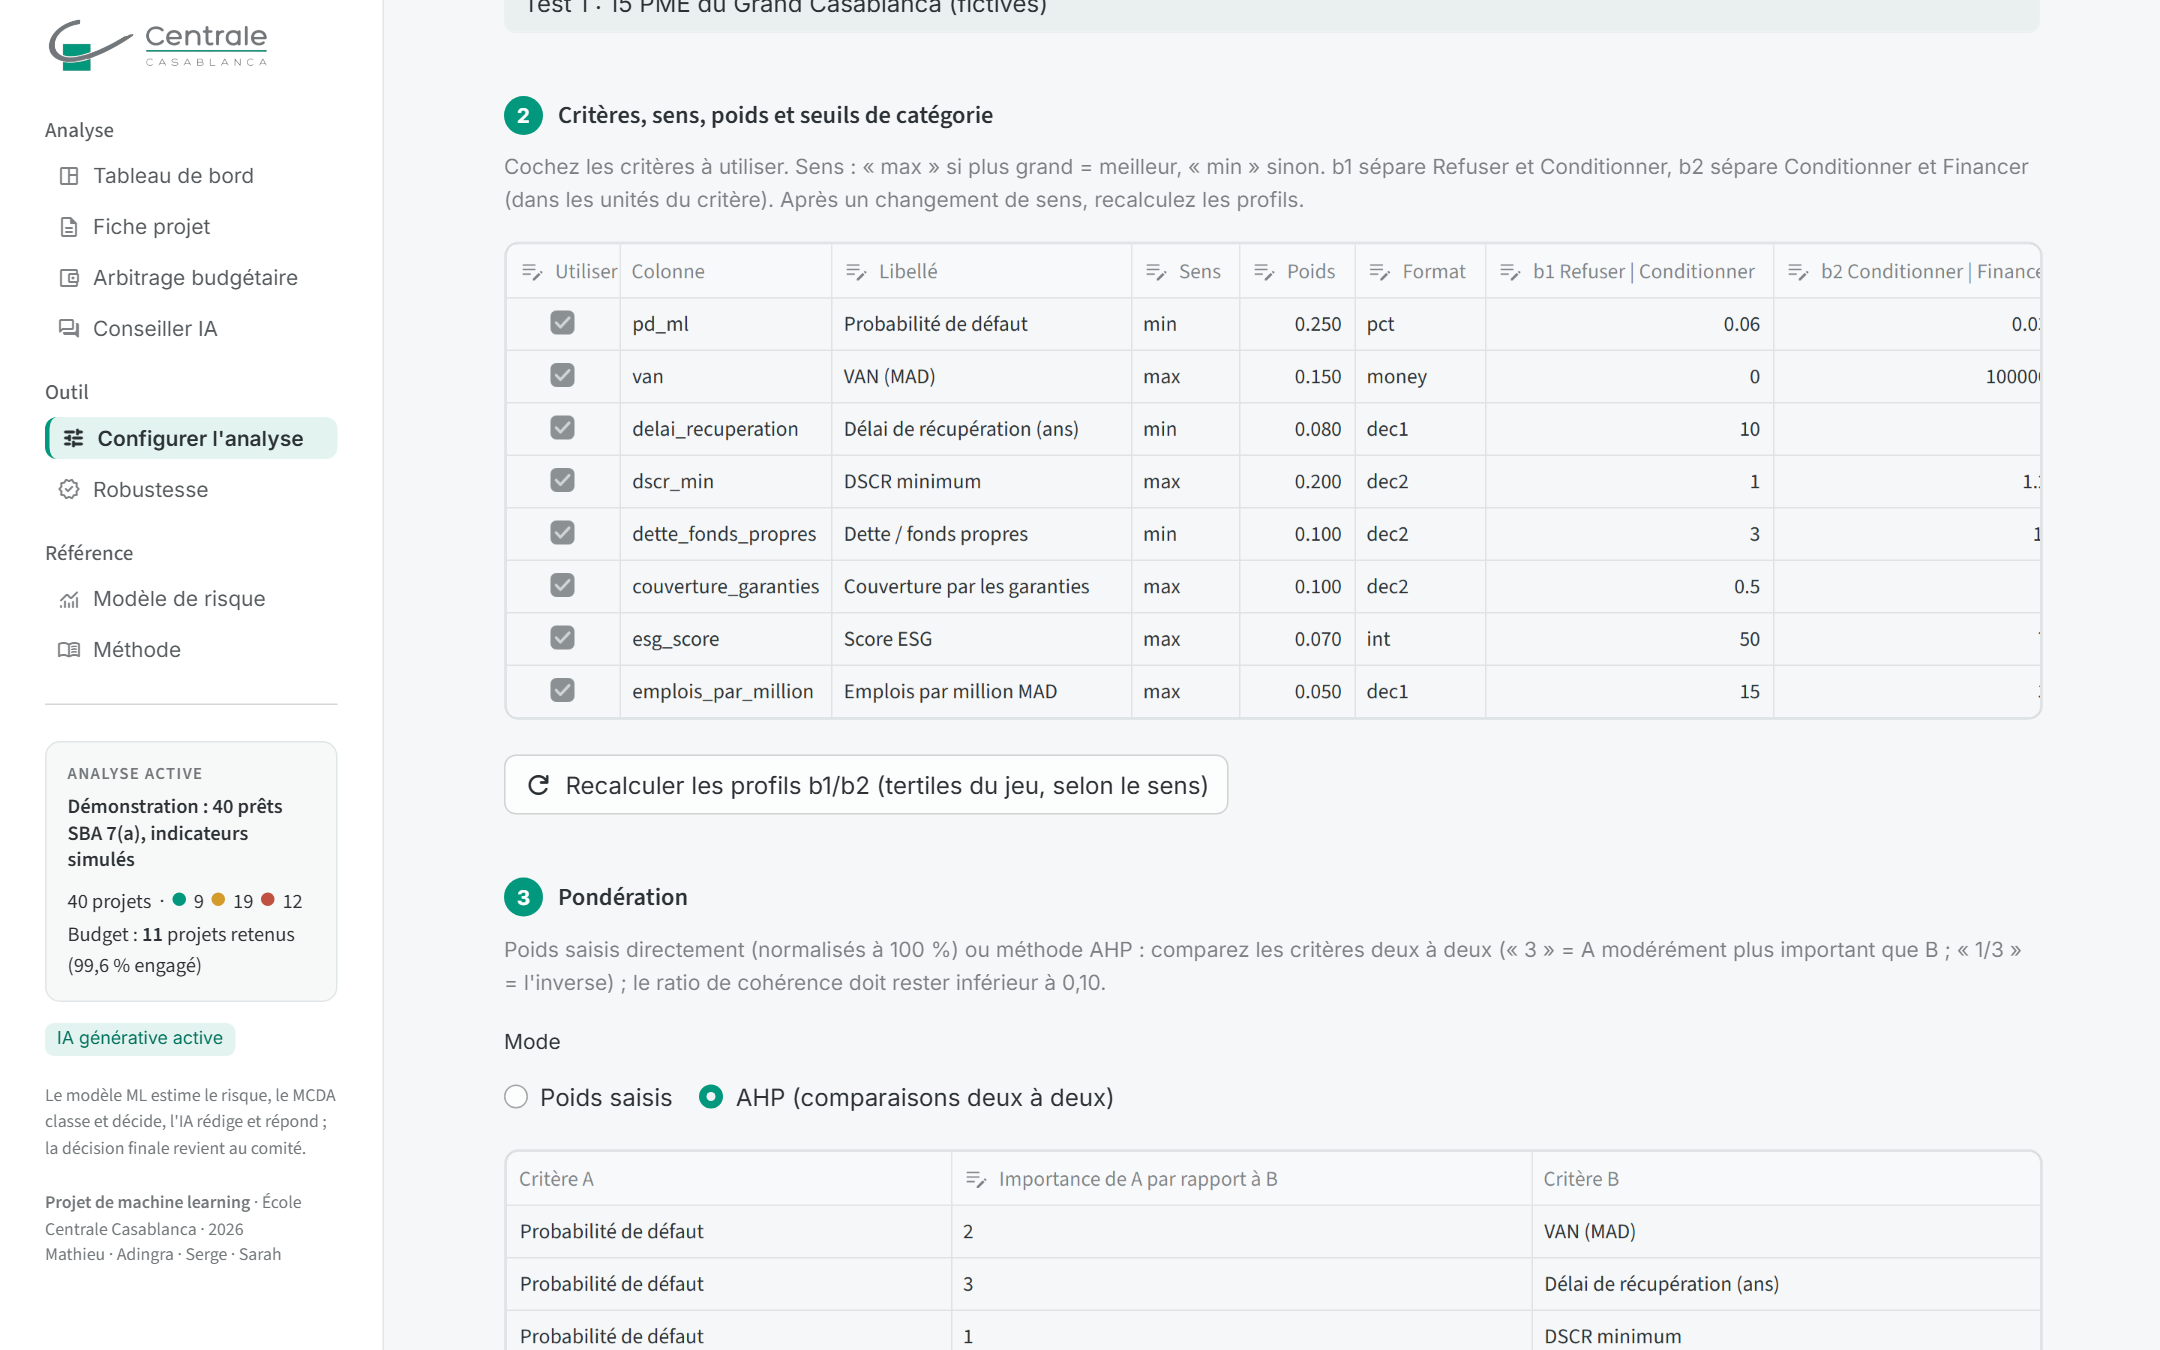
\includegraphics[width=\textwidth]{app_configurer.png}
  \caption{Page de configuration après import d'un jeu de 15 PME : tableau des critères, sens, poids et profils.}
  \label{fig:app-config}
\end{figure}

% ---------------------------------------------------------------------------------------------
\section{Reproductibilité et qualité}

Le dépôt GitHub contient le code source (\code{src/}), l'application (\code{app/}), les notebooks d'exploration et
de modélisation, les petits fichiers de résultats et un README qui décrit l'installation, l'ordre d'exécution, le
journal des données (source, taille, date) et chaque choix. Les données brutes, trop volumineuses, n'y sont pas : un
script vérifie leur présence et indique leurs adresses de téléchargement. Tous les tirages aléatoires ont une graine
fixe : deux exécutions donnent les mêmes chiffres. Trente tests automatiques vérifient notamment :

\begin{itemize}
  \item un exemple ELECTRE à trois projets calculé à la main (concordance, veto, classement) ;
  \item l'absence de variables qui fuient ou font double compte, et l'indépendance de la simulation vis-à-vis de
        l'issue réelle ;
  \item que le moteur générique reproduit exactement les résultats du pipeline sur la démonstration ;
  \item que l'arbitrage respecte toujours le budget, les bornes et le plafond sectoriel, pour les deux règles ;
  \item les outils du conseiller et la détection des chiffres et des méthodes inventés.
\end{itemize}

% =============================================================================================
\chapter{Discussion}\label{chap:discussion}

% ---------------------------------------------------------------------------------------------
\section{Justification des choix}

Le tableau~\ref{tab:choix} rassemble les principaux choix, l'alternative écartée et la raison du choix.

\begin{center}
\footnotesize
\begin{longtable}{>{\raggedright\arraybackslash}p{3.6cm}>{\raggedright\arraybackslash}p{3.2cm}>{\raggedright\arraybackslash}p{7.4cm}}
\caption{Choix de conception et justifications}\label{tab:choix}\\
\toprule
Choix & Alternative écartée & Raison \\
\midrule
\endfirsthead
\toprule
Choix & Alternative écartée & Raison \\
\midrule
\endhead
\bottomrule
\endfoot
Prêts SBA réels & données entièrement simulées & le risque doit être appris sur de vrais défauts ; données publiques et volumineuses \\
Défaut à 60 mois & perte à toute date & horizon d'un crédit d'investissement ; une perte tardive ne dépend plus du dossier \\
Séparation par année & tirage au hasard & une banque prédit le futur avec le passé \\
Test lu une seule fois & réglages vérifiés sur le test & éviter de choisir sans le vouloir ce qui réussit sur le test \\
Trois tranches de durée & durée exacte & la durée exacte est modifiée après un défaut (fuite) \\
Sans emplois ni garanties dans le modèle & toutes les variables & ce sont des critères MCDA : éviter le double comptage \\
Trois modèles, choix parmi les interprétables & choisir le plus performant & une banque doit expliquer un refus ; LightGBM mesure le prix de ce choix \\
Calibration isotonique & probabilités brutes & le MCDA utilise la probabilité ; les données d'entraînement incluent la crise \\
Pas de rééquilibrage des classes & sur- ou sous-échantillonnage & préserver des probabilités fidèles \\
Indicateurs simulés et documentés & indicateurs réels & aucune base ouverte ne relie comptes du projet et issue du prêt \\
AHP & poids posés directement & méthode reconnue qui contrôle la cohérence \\
Filtre éliminatoire & tout passer dans le classement & certaines conditions sont des couperets (ne pas pouvoir payer ses échéances) \\
Seuil de risque sur le taux de validation & taux d'entraînement & cohérence avec la période de calibration ; sinon le filtre est inopérant \\
ELECTRE III et TRI & somme pondérée & non-compensation : un risque élevé n'est pas racheté par une bonne VAN \\
Règle TRI pessimiste & règle optimiste & prudence bancaire \\
Profils absolus quand c'est possible & tertiles du lot & une catégorie doit traduire un standard, pas un rang \\
PROMETHEE II en complément & une seule méthode & vérifier que le classement ne dépend pas de la méthode \\
$\lambda$ entre 0,5 et 0,8 dans les scénarios & $\lambda$ jusqu'à 1 & $\lambda = 1$ exige l'unanimité, cas extrême montré à part \\
Arbitrage \og suivre le classement \fg{} & maximiser le nombre de projets & ne pas écarter le meilleur projet au profit de petits projets \\
Le LLM ne calcule pas & laisser le LLM analyser & un LLM peut inventer des chiffres ; chaque chiffre doit être traçable \\
Outils et vérificateur & confiance dans le LLM & chaque nombre est contrôlé automatiquement \\
Gemini gratuit & API payante & budget nul d'un projet étudiant \\
Application configurable & application figée & réutiliser la méthode sur de vraies données \\
\end{longtable}
\end{center}

% ---------------------------------------------------------------------------------------------
\section{Limites}

\paragraph{Indicateurs simulés.} C'est la limite principale : les catégories des 40 projets ne sont stables que dans
48\,\% des tirages de simulation. La démonstration valide la \emph{méthode} et la chaîne de décision, pas les catégories
de ces projets. Plusieurs paramètres de simulation sont des hypothèses non sourcées (croissance, horizon, valeur
résiduelle, bornes de dette et de garantie, centres ESG). Les 8 projets écartés pour un DSCR inférieur à 1 sont
exactement les 8 projets \og faibles \fg{} de la simulation : ce résultat découle de la construction.

\paragraph{Lien mécanique entre critères.} Le DSCR étant imposé, les flux sont proportionnels au service de la dette :
un prêt court, au service annuel élevé, a mécaniquement des flux plus forts, donc une VAN plus élevée et un délai plus
court. Comme les prêts courts sont aussi plus risqués pour le modèle, la probabilité de défaut est corrélée à la VAN et
au délai. Ce lien passe par la tranche de durée, connue à l'octroi, et non par l'issue réelle, mais il est un artefact
de la simulation.

\paragraph{Représentativité du modèle.} Le modèle a appris sur des prêts américains garantis par un organisme public ;
il ne représente pas directement un portefeuille bancaire marocain. Il sous-estime légèrement le risque de 2015-2016
(3,52\,\% prédit pour 4,25\,\% observé) en raison de la dérive entre périodes, et manque une majorité des défauts au
seuil F1.

\paragraph{Paramètres de la méthode.} Les jugements AHP ont été initialisés à partir des poids cibles : l'AHP en
vérifie surtout la cohérence, et devrait être rempli par des experts du crédit. Les seuils $q$, $p$, $v$ et certains
profils sont relatifs au lot : ajouter un projet peut les déplacer. Le classement ELECTRE III affiché est un ordre total
de lecture, qui résume les incomparabilités (signalées par les \og positions ambiguës \fg{}).

\paragraph{Agents fondés sur un LLM.} Le vérificateur contrôle les nombres et les noms de méthodes, pas le sens des
phrases : une explication peut rester approximative et demande une relecture humaine. L'offre gratuite de Gemini est
souvent saturée, ce qui allonge les réponses ; l'application reste utilisable sans LLM.

% ---------------------------------------------------------------------------------------------
\section{Écarts au cahier des charges}

\begin{itemize}
  \item \textbf{Agent extracteur} : non réalisé, nos dossiers étant des données structurées ; l'import de fichiers et
        le calcul automatique du risque en tiennent lieu.
  \item \textbf{TRI} : non calculé ; la VAN et le délai de récupération couvrent la rentabilité et la liquidité.
  \item \textbf{Durée du prêt} : remplacée par trois tranches à cause de la fuite détectée.
  \item \textbf{Seuil du filtre} : fondé sur le taux de défaut de validation plutôt que d'entraînement.
  \item \textbf{Variable de garantie} : retirée du modèle de risque pour éviter un double comptage.
\end{itemize}
Chacun de ces écarts est motivé par la qualité des résultats ou la cohérence de la méthode et est documenté.

% ---------------------------------------------------------------------------------------------
\section{Perspectives}

\begin{itemize}
  \item Appliquer l'outil à de vrais dossiers de crédit (bilans, plans de financement) pour remplacer la simulation.
  \item Réentraîner le modèle sur des données locales, ajouter des variables macroéconomiques et recalibrer
        régulièrement pour suivre la dérive.
  \item Faire remplir les comparaisons AHP par des analystes, et ajouter le TRI et une détection d'anomalies.
  \item Réaliser l'agent extracteur : un LLM qui lit des dossiers en PDF, remplit la matrice de performance en citant
        ses sources, et la soumet à la validation des analystes.
  \item Afficher le graphe de surclassement complet d'ELECTRE III et étendre l'arbitrage à plusieurs périodes.
\end{itemize}

% =============================================================================================
\chapter{Conclusion}\label{chap:conclusion}

Ce projet a construit un système d'aide à la décision d'investissement dans lequel chaque composant a un rôle unique et
vérifiable. Le risque de défaut est appris sur 910\,033 prêts réels, avec une séparation temporelle stricte et la
correction d'une fuite de données qui aurait gonflé artificiellement les performances. Parmi trois modèles, le modèle
interprétable EBM est retenu ; il atteint une AUROC de 0,778 sur des années futures, à 0,022 point d'un modèle opaque,
ce qui montre que l'exigence d'explicabilité d'une décision de crédit a ici un coût faible.

La décision repose sur une méthode multicritère non compensatoire. Avec des poids cohérents, un filtre éliminatoire et
des profils fondés sur des repères bancaires, ELECTRE TRI répartit les 40 projets en 9 à financer, 19 sous conditions et
12 refusés, ELECTRE III et PROMETHEE II s'accordent sur le classement, et les décisions de financement résistent aux
variations des paramètres de la méthode. Un agent d'arbitrage transforme ces catégories en une sélection qui respecte
le budget, les montants admissibles et la diversification sectorielle, et la comparaison de deux règles montre que le
choix de l'objectif d'optimisation est une décision de politique, pas un détail technique.

Les modèles de langage sont utilisés là où ils sont utiles et sûrs : rédiger une note et répondre à des questions,
sans jamais calculer, en appelant des fonctions déterministes dont chaque nombre est vérifié. Le système est déployé
dans une application réutilisable, testée et reproductible, qui peut évaluer n'importe quel jeu de projets.

La principale limite est connue et mesurée : les indicateurs financiers de la démonstration sont simulés, et les
catégories des projets en dépendent fortement. La prochaine étape naturelle est donc d'appliquer cet outil à de vrais
dossiers. Dans tous les cas, le système éclaire la décision sans la prendre : la décision finale reste celle du comité
d'investissement.


% =============================================================================================
% BIBLIOGRAPHIE ET ANNEXES
% =============================================================================================
\cleardoublepage
\phantomsection
\addcontentsline{toc}{chapter}{Bibliographie}
\bibliographystyle{plain}
\bibliography{references}

\appendix
% =============================================================================================
\chapter{Paramètres de la méthode}\label{ann:parametres}

\begin{table}[htbp]
\centering
\footnotesize\setlength{\tabcolsep}{4pt}
\caption{Matrice de comparaisons deux à deux de l'AHP (échelle de Saaty) ; $\lambda_{\max} = 8,091$, CR = 0,009}\label{tab:ahp}
\begin{tabular}{lcccccccc}
\toprule
 & PD & VAN & Délai & DSCR & D/FP & Gar. & ESG & Empl. \\
\midrule
PD & 1 & 2 & 3 & 1 & 3 & 3 & 4 & 5 \\
VAN & 1/2 & 1 & 2 & 1 & 2 & 2 & 2 & 3 \\
Délai & 1/3 & 1/2 & 1 & 1/3 & 1 & 1 & 1 & 2 \\
DSCR & 1 & 1 & 3 & 1 & 2 & 2 & 3 & 4 \\
D/FP & 1/3 & 1/2 & 1 & 1/2 & 1 & 1 & 2 & 2 \\
Gar. & 1/3 & 1/2 & 1 & 1/2 & 1 & 1 & 2 & 2 \\
ESG & 1/4 & 1/2 & 1 & 1/3 & 1/2 & 1/2 & 1 & 1 \\
Empl. & 1/5 & 1/3 & 1/2 & 1/4 & 1/2 & 1/2 & 1 & 1 \\
\bottomrule
\end{tabular}
\end{table}


\begin{table}[htbp]
\centering
\footnotesize\setlength{\tabcolsep}{4pt}
\caption{Paramètres sectoriels utilisés par la simulation (Damodaran, janvier 2026 ; croissance : hypothèse d'équipe)}\label{tab:damodaran}
\begin{tabular}{lccccc}
\toprule
Secteur Damodaran & Coût du capital & Coût de la dette & Bêta & Part de dette & Croissance (hyp.) \\
\midrule
Business \& Consumer Services & 7,2\,\% & 5,1\,\% & 0,89 & 16,5\,\% & 4\,\% \\
Engineering/Construction & 8,7\,\% & 5,3\,\% & 1,21 & 12,3\,\% & 3\,\% \\
Farming/Agriculture & 7,3\,\% & 5,3\,\% & 1,13 & 34,1\,\% & 2\,\% \\
Financial Svcs. (Non-bank \& Insurance) & 5,0\,\% & 5,1\,\% & 0,97 & 73,1\,\% & 4\,\% \\
Food Processing & 5,8\,\% & 5,1\,\% & 0,61 & 30,4\,\% & 3\,\% \\
Healthcare Support Services & 6,8\,\% & 5,3\,\% & 0,87 & 26,2\,\% & 4\,\% \\
Machinery & 7,7\,\% & 5,3\,\% & 0,96 & 12,8\,\% & 3\,\% \\
Real Estate (Operations \& Services) & 7,4\,\% & 5,3\,\% & 0,97 & 19,8\,\% & 3\,\% \\
Restaurant/Dining & 7,2\,\% & 5,1\,\% & 0,92 & 21,4\,\% & 3\,\% \\
Retail (Distributors) & 7,2\,\% & 5,1\,\% & 0,95 & 22,0\,\% & 3\,\% \\
Retail (General) & 7,3\,\% & 5,1\,\% & 0,81 & 7,4\,\% & 3\,\% \\
Transportation & 6,7\,\% & 5,1\,\% & 0,86 & 26,7\,\% & 3\,\% \\
\bottomrule
\end{tabular}
\end{table}


\chapter{Les 40 projets de démonstration}\label{ann:projets}

Les noms sont fictifs : l'activité vient du vrai code NAICS du prêt, le nom de famille d'une liste fixe. E-III et P-II
sont les rangs ELECTRE III et PROMETHEE II (\og -- \fg{} pour un projet écarté par le filtre) ; PD est la probabilité
de défaut estimée par l'EBM ; la dernière colonne indique si le projet est retenu par l'arbitrage sous budget
(5\,M\$, 20\,000\,\$ à 2\,M\$ par projet, 35\,\% au plus par secteur).

{\scriptsize\setlength{\tabcolsep}{3pt}
\begin{longtable}{p{3.7cm}p{2.5cm}lrrrrrrl}
\caption{Les 40 projets de démonstration (noms fictifs) : décision MCDA et sélection sous budget}\label{tab:projets}\\
\toprule
Projet & Secteur & Décision & E-III & P-II & PD & DSCR & VAN & Montant & Budget \\
\midrule
\endfirsthead
\toprule
Projet & Secteur & Décision & E-III & P-II & PD & DSCR & VAN & Montant & Budget \\
\midrule
\endhead
\bottomrule
\endfoot
Studio de développement logiciel Murphy & Business \& Consumer Services & Financer & 1 & 1 & 0,9\,\% & 1,61 & 3\,286\,k\$ & 1\,700\,k\$ & oui \\
Atelier d'insertion professionnelle Foster & Healthcare Support Services & Financer & 2 & 2 & 0,4\,\% & 1,76 & -23\,k\$ & 110\,k\$ & oui \\
Brasserie artisanale Garcia & Food Processing & Financer & 5 & 10 & 0,9\,\% & 1,14 & 23\,k\$ & 50\,k\$ & oui \\
Conseil en investissement Park & Financial Svcs. & Financer & 6 & 6 & 3,4\,\% & 1,91 & 2\,320\,k\$ & 820\,k\$ & oui \\
Cabinet dentaire Kowalski & Healthcare Support Services & Financer & 9 & 5 & 1,0\,\% & 1,36 & 655\,k\$ & 610\,k\$ & oui \\
Clinique privée Nguyen & Healthcare Support Services & Financer & 10 & 17 & 3,4\,\% & 1,18 & 339\,k\$ & 350\,k\$ & oui \\
Grossiste en fleurs Sullivan & Retail (Distributors) & Financer & 11 & 9 & 1,3\,\% & 1,44 & 418\,k\$ & 350\,k\$ & oui \\
Pompes funèbres Price & Business \& Consumer Services & Financer & 14 & 18 & 2,2\,\% & 1,31 & 83\,k\$ & 168\,k\$ & non \\
Travaux routiers Romano & Engineering/Construction & Financer & 24 & 28 & 3,4\,\% & 1,03 & 6\,k\$ & 40\,k\$ & oui \\
Bureau d'ingénierie Dubois & Business \& Consumer Services & Sous conditions & 3 & 11 & 0,9\,\% & 1,36 & 35\,k\$ & 50\,k\$ & oui \\
Entreprise de travaux spécialisés Brooks & Engineering/Construction & Sous conditions & 4 & 4 & 0,4\,\% & 1,93 & 2\,k\$ & 25\,k\$ & oui \\
Transports routiers Carter & Transportation & Sous conditions & 7 & 3 & 1,1\,\% & 1,46 & 1\,873\,k\$ & 876\,k\$ & oui \\
Cabinet de kinésithérapie Schmidt & Healthcare Support Services & Sous conditions & 8 & 7 & 0,4\,\% & 1,26 & -261\,k\$ & 603\,k\$ & non \\
Cabinet dentaire Baker & Healthcare Support Services & Sous conditions & 12 & 13 & 0,4\,\% & 1,27 & -172\,k\$ & 800\,k\$ & non \\
Restaurant Moreau & Restaurant/Dining & Sous conditions & 13 & 14 & 4,2\,\% & 1,67 & 49\,k\$ & 30\,k\$ & non \\
Cabinet de spécialistes Ramirez & Healthcare Support Services & Sous conditions & 15 & 15 & 2,2\,\% & 1,38 & 339\,k\$ & 350\,k\$ & non \\
Exploitation forestière Novak & Farming/Agriculture & Sous conditions & 16 & 8 & 0,9\,\% & 1,32 & 25\,k\$ & 40\,k\$ & non \\
Garde-meubles Silva & Real Estate (Operations \& Services) & Sous conditions & 17 & 24 & 2,2\,\% & 1,04 & -52\,k\$ & 218\,k\$ & non \\
Transports locaux Lopez & Transportation & Sous conditions & 18 & 16 & 3,5\,\% & 1,65 & 106\,k\$ & 44\,k\$ & non \\
Boutique d'accessoires Delgado & Retail (General) & Sous conditions & 19 & 20 & 3,0\,\% & 1,42 & 30\,k\$ & 30\,k\$ & non \\
Station de lavage Rivera & Business \& Consumer Services & Sous conditions & 20 & 22 & 5,2\,\% & 1,68 & 86\,k\$ & 75\,k\$ & non \\
Entreprise de gros œuvre Fischer & Engineering/Construction & Sous conditions & 21 & 12 & 0,9\,\% & 1,43 & -96\,k\$ & 125\,k\$ & non \\
Fret longue distance Cohen & Transportation & Sous conditions & 22 & 21 & 2,2\,\% & 1,47 & 14\,k\$ & 10\,k\$ & non \\
Locaux commerciaux Reyes & Real Estate (Operations \& Services) & Sous conditions & 23 & 19 & 1,3\,\% & 1,29 & -38\,k\$ & 1\,000\,k\$ & non \\
Snack Tanaka & Restaurant/Dining & Sous conditions & 25 & 26 & 2,9\,\% & 1,10 & -57\,k\$ & 125\,k\$ & non \\
Garde-meubles Grant & Real Estate (Operations \& Services) & Sous conditions & 27 & 25 & 0,9\,\% & 1,23 & -1\,702\,k\$ & 5\,000\,k\$ & non \\
Cabinet de conseil Patel & Business \& Consumer Services & Sous conditions & 28 & 27 & 3,4\,\% & 1,18 & 20\,k\$ & 19\,k\$ & non \\
Studio de design graphique Walsh & Business \& Consumer Services & Sous conditions & 29 & 29 & 5,2\,\% & 1,16 & 108\,k\$ & 150\,k\$ & non \\
Restaurant Bennett & Restaurant/Dining & Refuser & 26 & 23 & 0,8\,\% & 1,05 & -192\,k\$ & 403\,k\$ & non \\
Centre de soins paramédicaux Miller & Healthcare Support Services & Refuser & -- & -- & 3,4\,\% & 0,92 & 9\,k\$ & 15\,k\$ & non \\
Atelier de métallurgie Larsen & Machinery & Refuser & -- & -- & 1,5\,\% & 0,86 & -38\,k\$ & 75\,k\$ & non \\
Fret longue distance O'Brien & Transportation & Refuser & -- & -- & 1,3\,\% & 0,85 & -134\,k\$ & 317\,k\$ & non \\
Paysagiste Wright & Business \& Consumer Services & Refuser & -- & -- & 1,1\,\% & 0,88 & 15\,k\$ & 33\,k\$ & non \\
Cave à vins Hayes & Retail (General) & Refuser & -- & -- & 3,5\,\% & 0,88 & 47\,k\$ & 50\,k\$ & non \\
Constructeur de maisons Chen & Engineering/Construction & Refuser & -- & -- & 14,1\,\% & 1,46 & 23\,k\$ & 10\,k\$ & non \\
Concession nautique Ortiz & Retail (General) & Refuser & -- & -- & 1,3\,\% & 0,92 & -45\,k\$ & 150\,k\$ & non \\
Institut de bien-être Okafor & Business \& Consumer Services & Refuser & -- & -- & 0,8\,\% & 0,83 & -6\,k\$ & 78\,k\$ & non \\
Snack Rossi & Restaurant/Dining & Refuser & -- & -- & 9,6\,\% & 1,41 & 81\,k\$ & 53\,k\$ & non \\
Entreprise de travaux spécialisés Hernandez & Engineering/Construction & Refuser & -- & -- & 8,9\,\% & 1,96 & 205\,k\$ & 140\,k\$ & non \\
Agence d'assurances Kim & Financial Svcs. & Refuser & -- & -- & 2,2\,\% & 0,99 & 673\,k\$ & 950\,k\$ & non \\
\end{longtable}}


\chapter{Reproduction}\label{ann:reproduction}

\section{Structure du dépôt}

\begin{table}[htbp]
\centering\small
\caption{Structure du dépôt GitHub}\label{tab:depot}
\begin{tabularx}{\textwidth}{>{\ttfamily}p{3.6cm}X}
\toprule
\normalfont Dossier & Contenu \\
\midrule
data/ & données brutes et intermédiaires (non versionnées) et petits fichiers de résultats \\
src/ & pipeline (préparation, modèles, interprétabilité, simulation, MCDA, arbitrage), moteur générique, agents \\
app/ & application Streamlit (une page par fichier, logo, thème) \\
notebooks/ & audit et exploration, régression logistique, comparaison des modèles, interprétabilité \\
models/, reports/, params/ & modèle entraîné, métriques et figures, paramètres (AHP, profils, filtre, arbitrage) \\
exemples/ & jeux de test de l'outil réutilisable et leurs configurations \\
tests/ & 30 tests automatiques \\
rapport/ & ce rapport (LaTeX), ses figures et ses tableaux générés \\
\bottomrule
\end{tabularx}
\end{table}

\section{Commandes}

\begin{lstlisting}
pip install -r requirements.txt -r requirements-dev.txt
python scripts/download_data.py        # verifie les donnees et donne les liens
cd src
python data_prep.py                    # cible default_60m, separation temporelle
python models.py                       # logistique, EBM, LightGBM, calibration
python export_pd.py                    # probabilite de defaut du test
python eda.py                          # figures d'analyse exploratoire
python simulate.py                     # 40 projets, indicateurs simules
python project_scores.py               # table des 8 criteres
python interpret_model.py              # permutation, effets EBM, SHAP
python run_mcda.py                     # AHP, filtre, ELECTRE, PROMETHEE, arbitrage
python sensibilite_simulation.py       # 20 tirages de simulation
python rapport_assets.py               # figures et tableaux du rapport
cd ..
python -m pytest tests -q
streamlit run app/app.py
\end{lstlisting}


\end{document}
